\documentclass{article}

\PassOptionsToPackage{numbers,sort&compress}{natbib}
\usepackage{tackling_climate_workshop_style}
\usepackage{fontspec}
\usepackage{polyglossia}
\setmainlanguage{russian}
\setotherlanguage{english}
\setmainfont{Liberation Serif}
\setsansfont{Liberation Sans}
\setmonofont{Liberation Mono}
\usepackage{hyperref}
\hypersetup{hidelinks}
\usepackage{url}
\usepackage{graphicx}
\usepackage{booktabs}
\usepackage{tabularx}
\usepackage{array}
\usepackage{amsmath,amssymb}
\usepackage{xcolor}
\usepackage{tikz}
\usetikzlibrary{arrows.meta,positioning,calc}

\makeatletter
\renewenvironment{abstract}%
{\vskip 0.075in\centerline{\large\bf Аннотация}\vspace{0.5ex}\begin{quote}}%
{\par\end{quote}\vskip 1ex}
\makeatother

\definecolor{datablue}{HTML}{DCEAF7}
\definecolor{climorange}{HTML}{FCE3C3}
\definecolor{modelgreen}{HTML}{D9EAD3}
\definecolor{resultpurple}{HTML}{E7D9F2}
\definecolor{inkblue}{HTML}{365A73}
\definecolor{warmline}{HTML}{B46A2C}
\definecolor{metricblue}{HTML}{E8EEF3}
\newcolumntype{Y}{>{\raggedright\arraybackslash}X}
\newcommand{\rmse}{\operatorname{RMSE}}
\newcommand{\acc}{\operatorname{ACC}}

\title{Климатологический патчинг выявляет межпеременные зависимости в нейросетевых прогнозах погоды}
\author{Анонимные авторы}

\begin{document}
\maketitle

\begin{abstract}
Метрики качества прогноза не показывают, какие входные поля нужны модели, а какие она восстанавливает из контекста. Для безградиентного аудита одно атмосферное поле заменяется климатологией, согласованной по дню года и часу UTC; остальные входы фиксируются. Повторение интервенции для 19 полей дает направленную матрицу чувствительности $19\times19$. На 48 сезонно сбалансированных инициализациях 2024 года корреляция внедиагональных элементов Aurora и Pangu-Weather равна $r=0.913$, хотя отдельные зависимости сильно асимметричны. На +6 ч замена $Z850$ изменяет $V850$ примерно в девять раз сильнее, чем обратная замена, в обеих моделях. Шеститочечная доза $Z1000$ растет без насыщения и различает модели: наклон $T1000$ у Aurora снижается с $0.690$ на +6 ч до $0.217$ на +24 ч, а у Pangu-Weather растет с $0.406$ до $0.614$. При полной замене RMSE $T1000$ на +6 ч возрастает соответственно в $6.02$ и $3.35$ раза. Эти значения описывают конечный стресс-тест фиксированной модели и не устанавливают причинные связи в атмосфере.
\end{abstract}

\section{Введение}

Pangu-Weather и Aurora строят глобальные прогнозы высокого разрешения с низкой стоимостью инференса~\citep{bi2023pangu,bodnar2025aurora}. Агрегированные метрики сводят многомерное поведение к нескольким числам. При одинаковом качестве модели могут опираться на разные входные каналы, восстанавливать отсутствующее поле по соседним уровням или переносить ошибку одного поля на многие выходы. Такая диагностика нужна до включения модели в системы раннего предупреждения и климатические сервисы~\citep{wmo2025earlywarning}. Методы интерпретации используют градиенты, возмущения и анализ представлений~\citep{yang2024survey}; градиенты дороги для миллиардных моделей, а корреляции не задают направление зависимости.

В эксперименте одно входное поле заменяется его ожидаемым сезонно-суточным состоянием, после чего измеряется отклик каждого выхода. Анализ охватывает 19 входов и выходов, Aurora и Pangu-Weather, а также заблаговременности 6 и 24 ч. Плавная доза проверяет пригодность полной замены как конечной точки; пространственные композиты локализуют добавленную ошибку. Метод предназначен для аудита прогнозных компонентов в задачах адаптации и раннего предупреждения. Он не решает задачу климатической атрибуции и не оценивает меры по снижению выбросов.

\section{Методы}

\subsection{Данные, модели и выборка}

ERA5 используется для начальных состояний и верификации~\citep{hersbach2020era5}; климатология WeatherBench 2 согласована по дню года и часу UTC и рассчитана за 1990--2019 годы~\citep{rasp2024weatherbench2}. Мы оцениваем Aurora (1.3 млрд параметров, два входных момента) и Pangu-Weather (256 млн, один момент) на сетках $0.25^\circ$. Аудит охватывает 48 инициализаций 2024 года: четыре даты в каждом месяце, часы 00/06/12/18 UTC сбалансированы. Рассматриваются 19 полей: MSLP, $u/v$ на 10 м, температура на 2 м, а также геопотенциал $Z$, удельная влажность $Q$, температура $T$ и ветер $u/v$ на 1000, 850 и 500 гПа. У Aurora заменяются оба входных снимка.

\begin{figure}[t]
\centering
\resizebox{\linewidth}{!}{%
\begin{tikzpicture}[
  every node/.style={font=\scriptsize,align=center,inner sep=4pt},
  source/.style={draw=inkblue,rounded corners=2.5pt,fill=datablue,minimum width=2.35cm,minimum height=0.82cm,line width=0.65pt},
  clim/.style={draw=warmline,rounded corners=2.5pt,fill=climorange,minimum width=2.35cm,minimum height=0.82cm,line width=0.65pt},
  patch/.style={draw=warmline,rounded corners=2.5pt,fill=white,minimum width=3.10cm,minimum height=1.02cm,line width=0.75pt},
  model/.style={draw=green!45!black,rounded corners=2.5pt,fill=modelgreen,minimum width=2.25cm,minimum height=0.86cm,line width=0.65pt},
  forecast/.style={draw=violet!55!black,rounded corners=2.5pt,fill=resultpurple,minimum width=2.20cm,minimum height=0.86cm,line width=0.65pt},
  metric/.style={draw=inkblue,rounded corners=2.5pt,fill=metricblue,minimum width=2.65cm,minimum height=1.02cm,line width=0.75pt},
  result/.style={draw=violet!55!black,rounded corners=2.5pt,fill=resultpurple,minimum width=2.70cm,minimum height=1.02cm,line width=0.75pt},
  flow/.style={-{Latex[length=2.2mm,width=1.45mm]},draw=black!65,line width=0.75pt,rounded corners=3pt},
  patchflow/.style={flow,draw=warmline},
  lane/.style={font=\tiny\bfseries,anchor=west,inner sep=0pt}
]
  \node[lane,text=inkblue] at (-1.15,1.72) {БАЗОВЫЙ ПРОГНОЗ};
  \node[lane,text=warmline] at (-1.15,-0.48) {ИНТЕРВЕНЦИЯ};
  \node[source] (x) at (0,1.08) {состояние ERA5 $\mathbf{x}(t)$\\19 полей};
  \node[clim] (c) at (0,-1.18) {климатология WB2 $\mathbf{c}(d,h)$\\сезон + час UTC};
  \node[model] (mb) at (5.90,1.08) {фиксированная $f_\theta$\\базовый прогноз};
  \node[patch] (p) at (3.05,-1.18) {$x_v^{(\alpha)}=(1-\alpha)x_v+\alpha c_v$\\$x_{j\ne v}^{(\alpha)}=x_j$};
  \node[model] (mp) at (5.90,-1.18) {та же $f_\theta$\\прогноз с патчем};
  \node[forecast] (yb) at (8.45,1.08) {$\hat y_u^{(0)}$\\+6 ч, +24 ч};
  \node[forecast] (yp) at (8.45,-1.18) {$\hat y_u^{(v,\alpha)}$\\+6 ч, +24 ч};
  \node[metric] (m) at (11.40,0) {$S_{vu}$ и $\Delta\acc_{vu}$\\веса по площади; ERA5};
  \node[result] (r) at (14.70,0) {матрицы $19\!\times\!19$\\дозы; карты ошибки};
  \draw[flow] (x.east) -- (mb.west);
  \draw[flow] (mb.east) -- (yb.west);
  \draw[patchflow] (x.south) -- ++(0,-0.43) -| (p.north);
  \draw[patchflow] (c.east) -- (p.west);
  \draw[patchflow] (p.east) -- (mp.west);
  \draw[patchflow] (mp.east) -- (yp.west);
  \draw[flow] (yb.east) -- (m.north west);
  \draw[patchflow] (yp.east) -- (m.south west);
  \draw[flow] (m.east) -- (r.west);
\end{tikzpicture}}
\caption{Климатологический патчинг использует парные прогнозы. Дата, веса модели и 18 незамененных полей фиксированы. Полная замена ($\alpha=1$) задает элемент матрицы; шесть значений $\alpha$ показывают траекторию отклика.}
\label{fig:method}
\end{figure}

\subsection{Интервенция и метрики}

Оператор $P_v$ заменяет полное глобальное поле $v$ климатологией. Для выходного поля $u$, заблаговременности $\tau$ и набора инициализаций $\mathcal D$ вычисляются
\begin{align}
S_{vu}(\tau)&=\frac{1}{|\mathcal D|}\sum_{t\in\mathcal D}
\frac{\rmse_w(\hat y_u^{(v)},\hat y_u^{(0)})}{\sigma_w(y_u)}, \\
\Delta\acc_{vu}(\tau)&=\frac{1}{|\mathcal D|}\sum_{t\in\mathcal D}
\left[\acc_w(\hat y_u^{(v)},y_u,c_u)-\acc_w(\hat y_u^{(0)},y_u,c_u)\right].
\end{align}
Во всех пространственных суммах используются нормированные веса $\cos\phi$. $S$ измеряет сдвиг прогноза, отрицательное $\Delta\acc$ соответствует потере качества по аномалиям. В эксперименте с дозой $Z1000$ заменяется при $\alpha\in\{0,.2,.4,.6,.8,1\}$, а ошибка нормируется как $\rmse_w/\sigma_w(y-c)$; единица соответствует климатологическому прогнозу без навыка. Интервенция показывает, как обученная сеть использует вход, но не устанавливает физическую причинность.

\section{Результаты}

\subsection{Корреляция как описательный baseline}

Матрица корреляций аномалий 69 выходных каналов Pangu содержит вертикально когерентные блоки геопотенциала, влажности, температуры и ветра (приложение~\ref{app:figures}). Разность с ERA5 зависит от синоптического случая. Локальные корреляции одного момента в скользящем окне шумны на гладких полях. Обе диагностики сохранены для проверки ассоциаций; направление оценивается патчингом.

\begin{figure}[t]
\centering
\begin{minipage}[t]{0.485\linewidth}
  \centering
  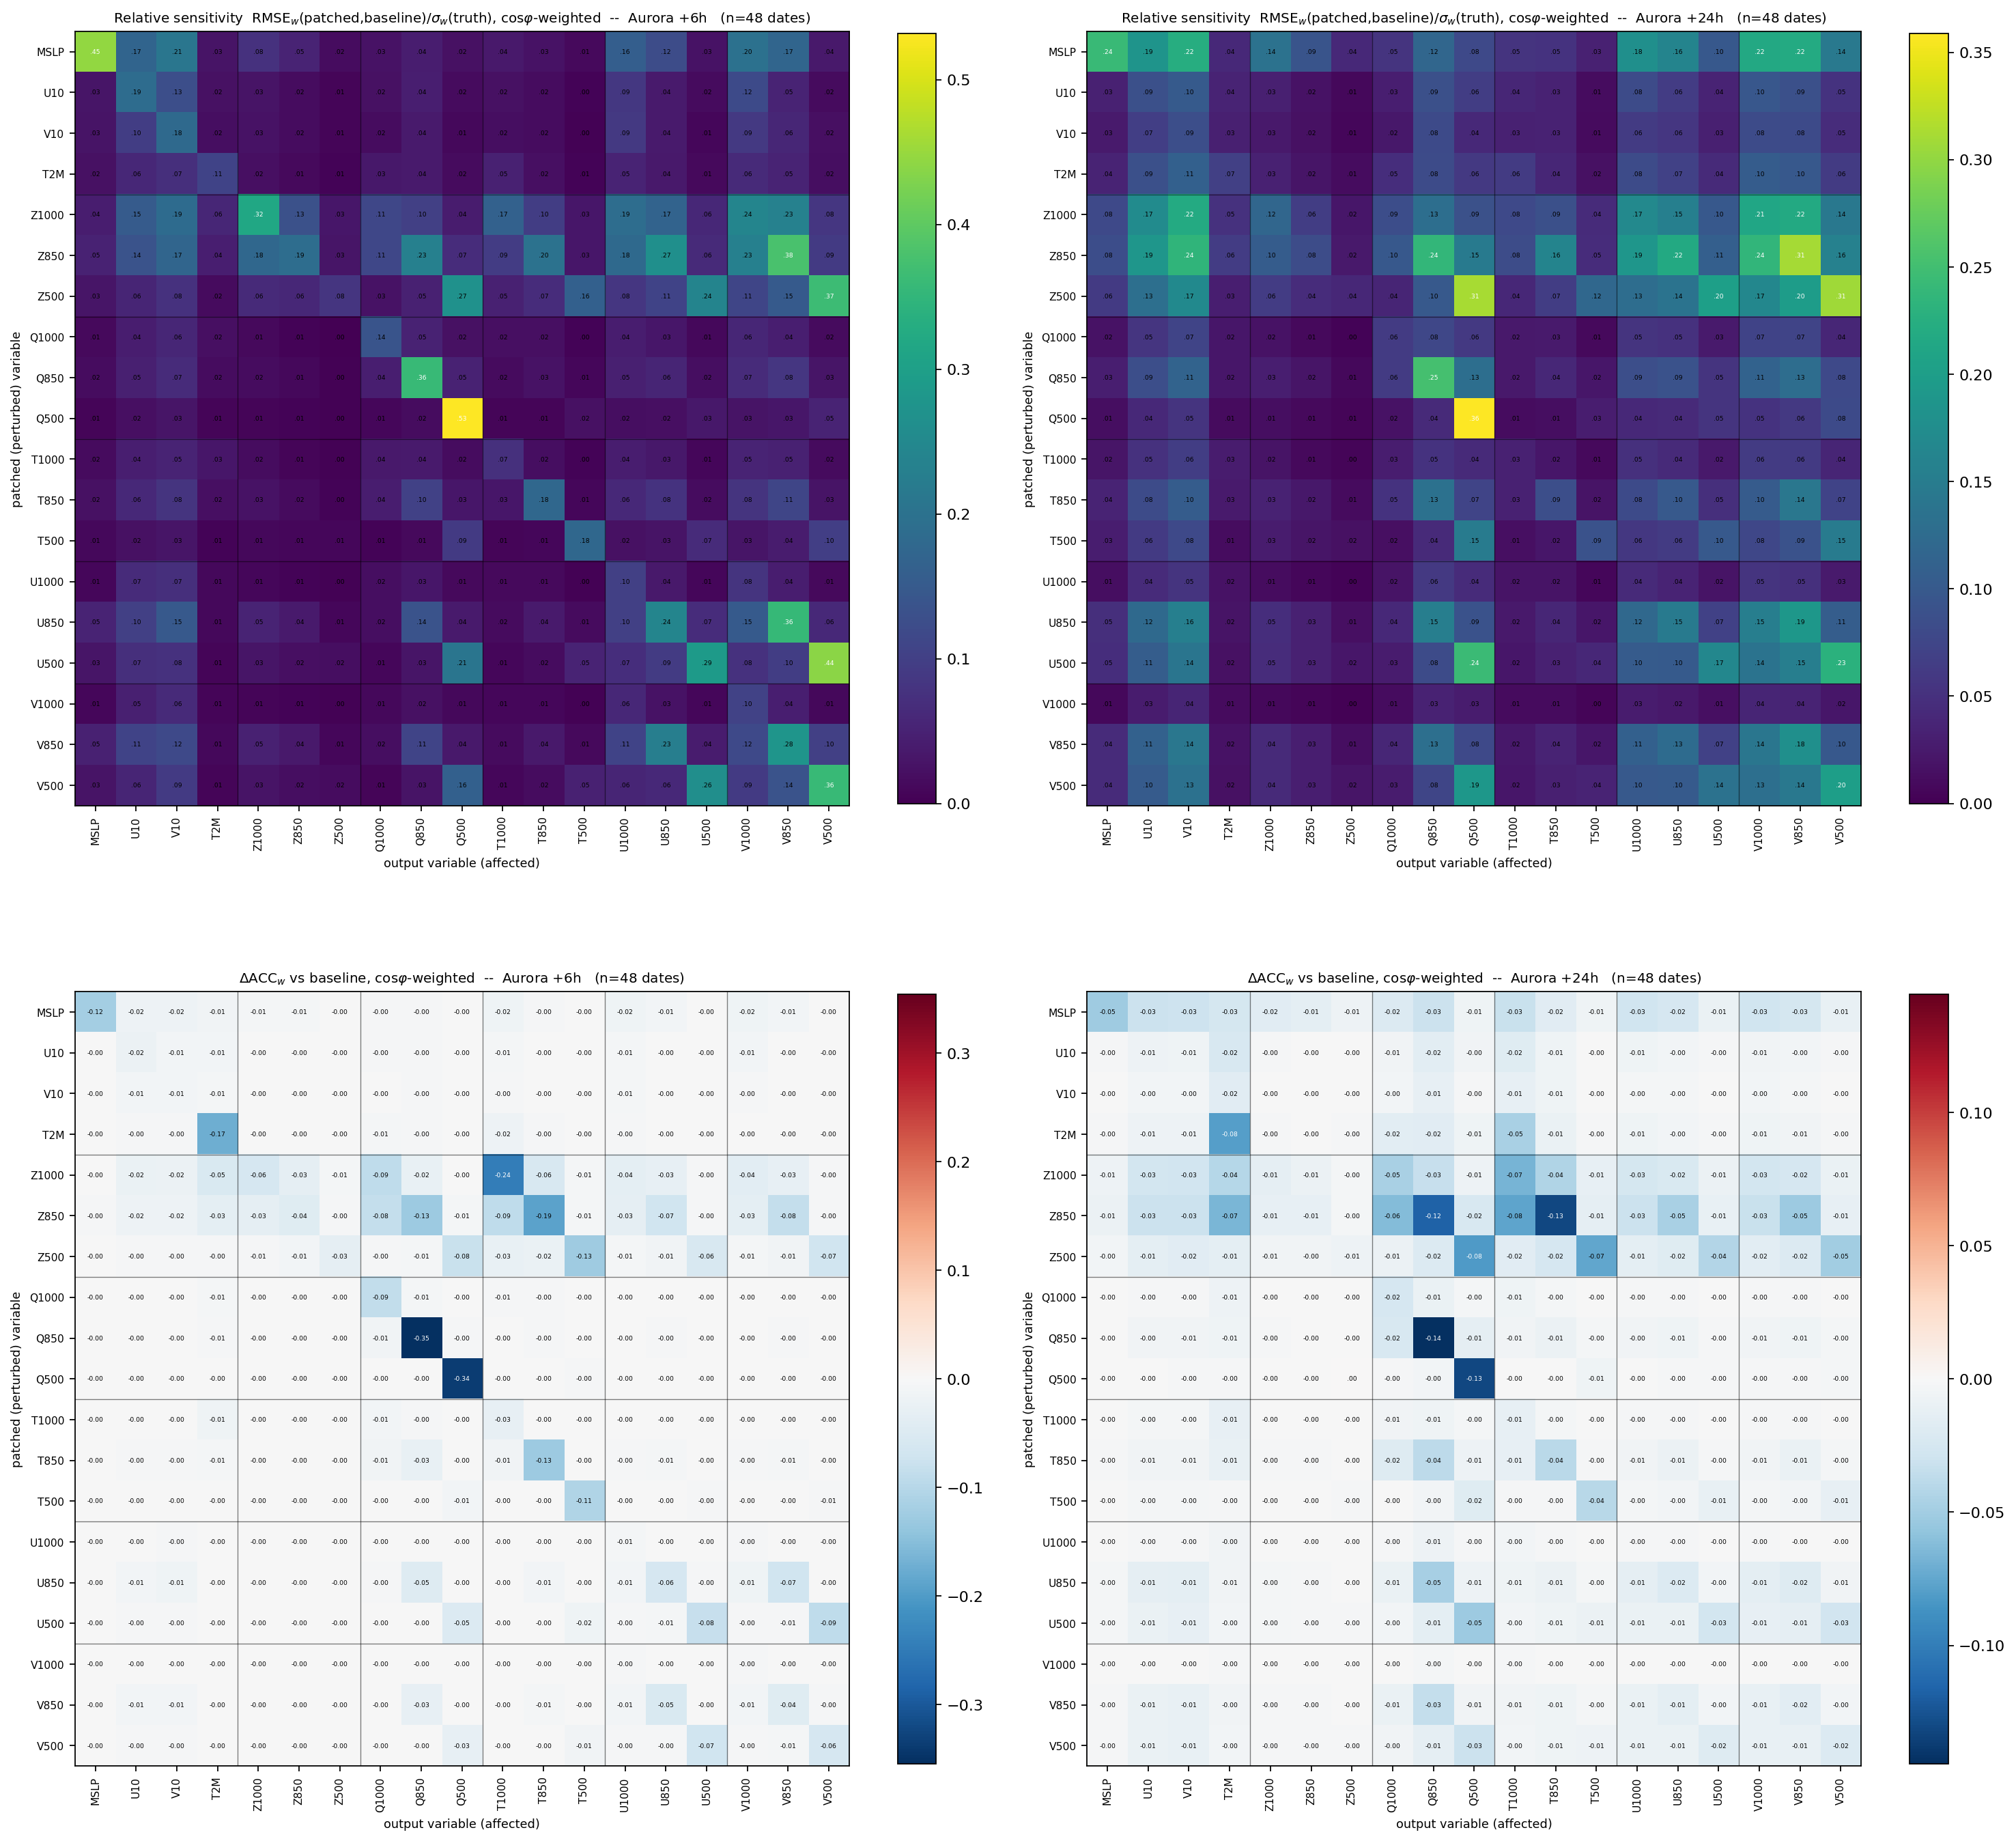
\includegraphics[width=\linewidth,trim=0.30in 8.65in 10.48in 0.12in,clip]{../../figures/patching_matrices/matrix_19var_aurora_n48_weighted.png}
  \\(a) Aurora, +6 ч
\end{minipage}\hfill
\begin{minipage}[t]{0.485\linewidth}
  \centering
  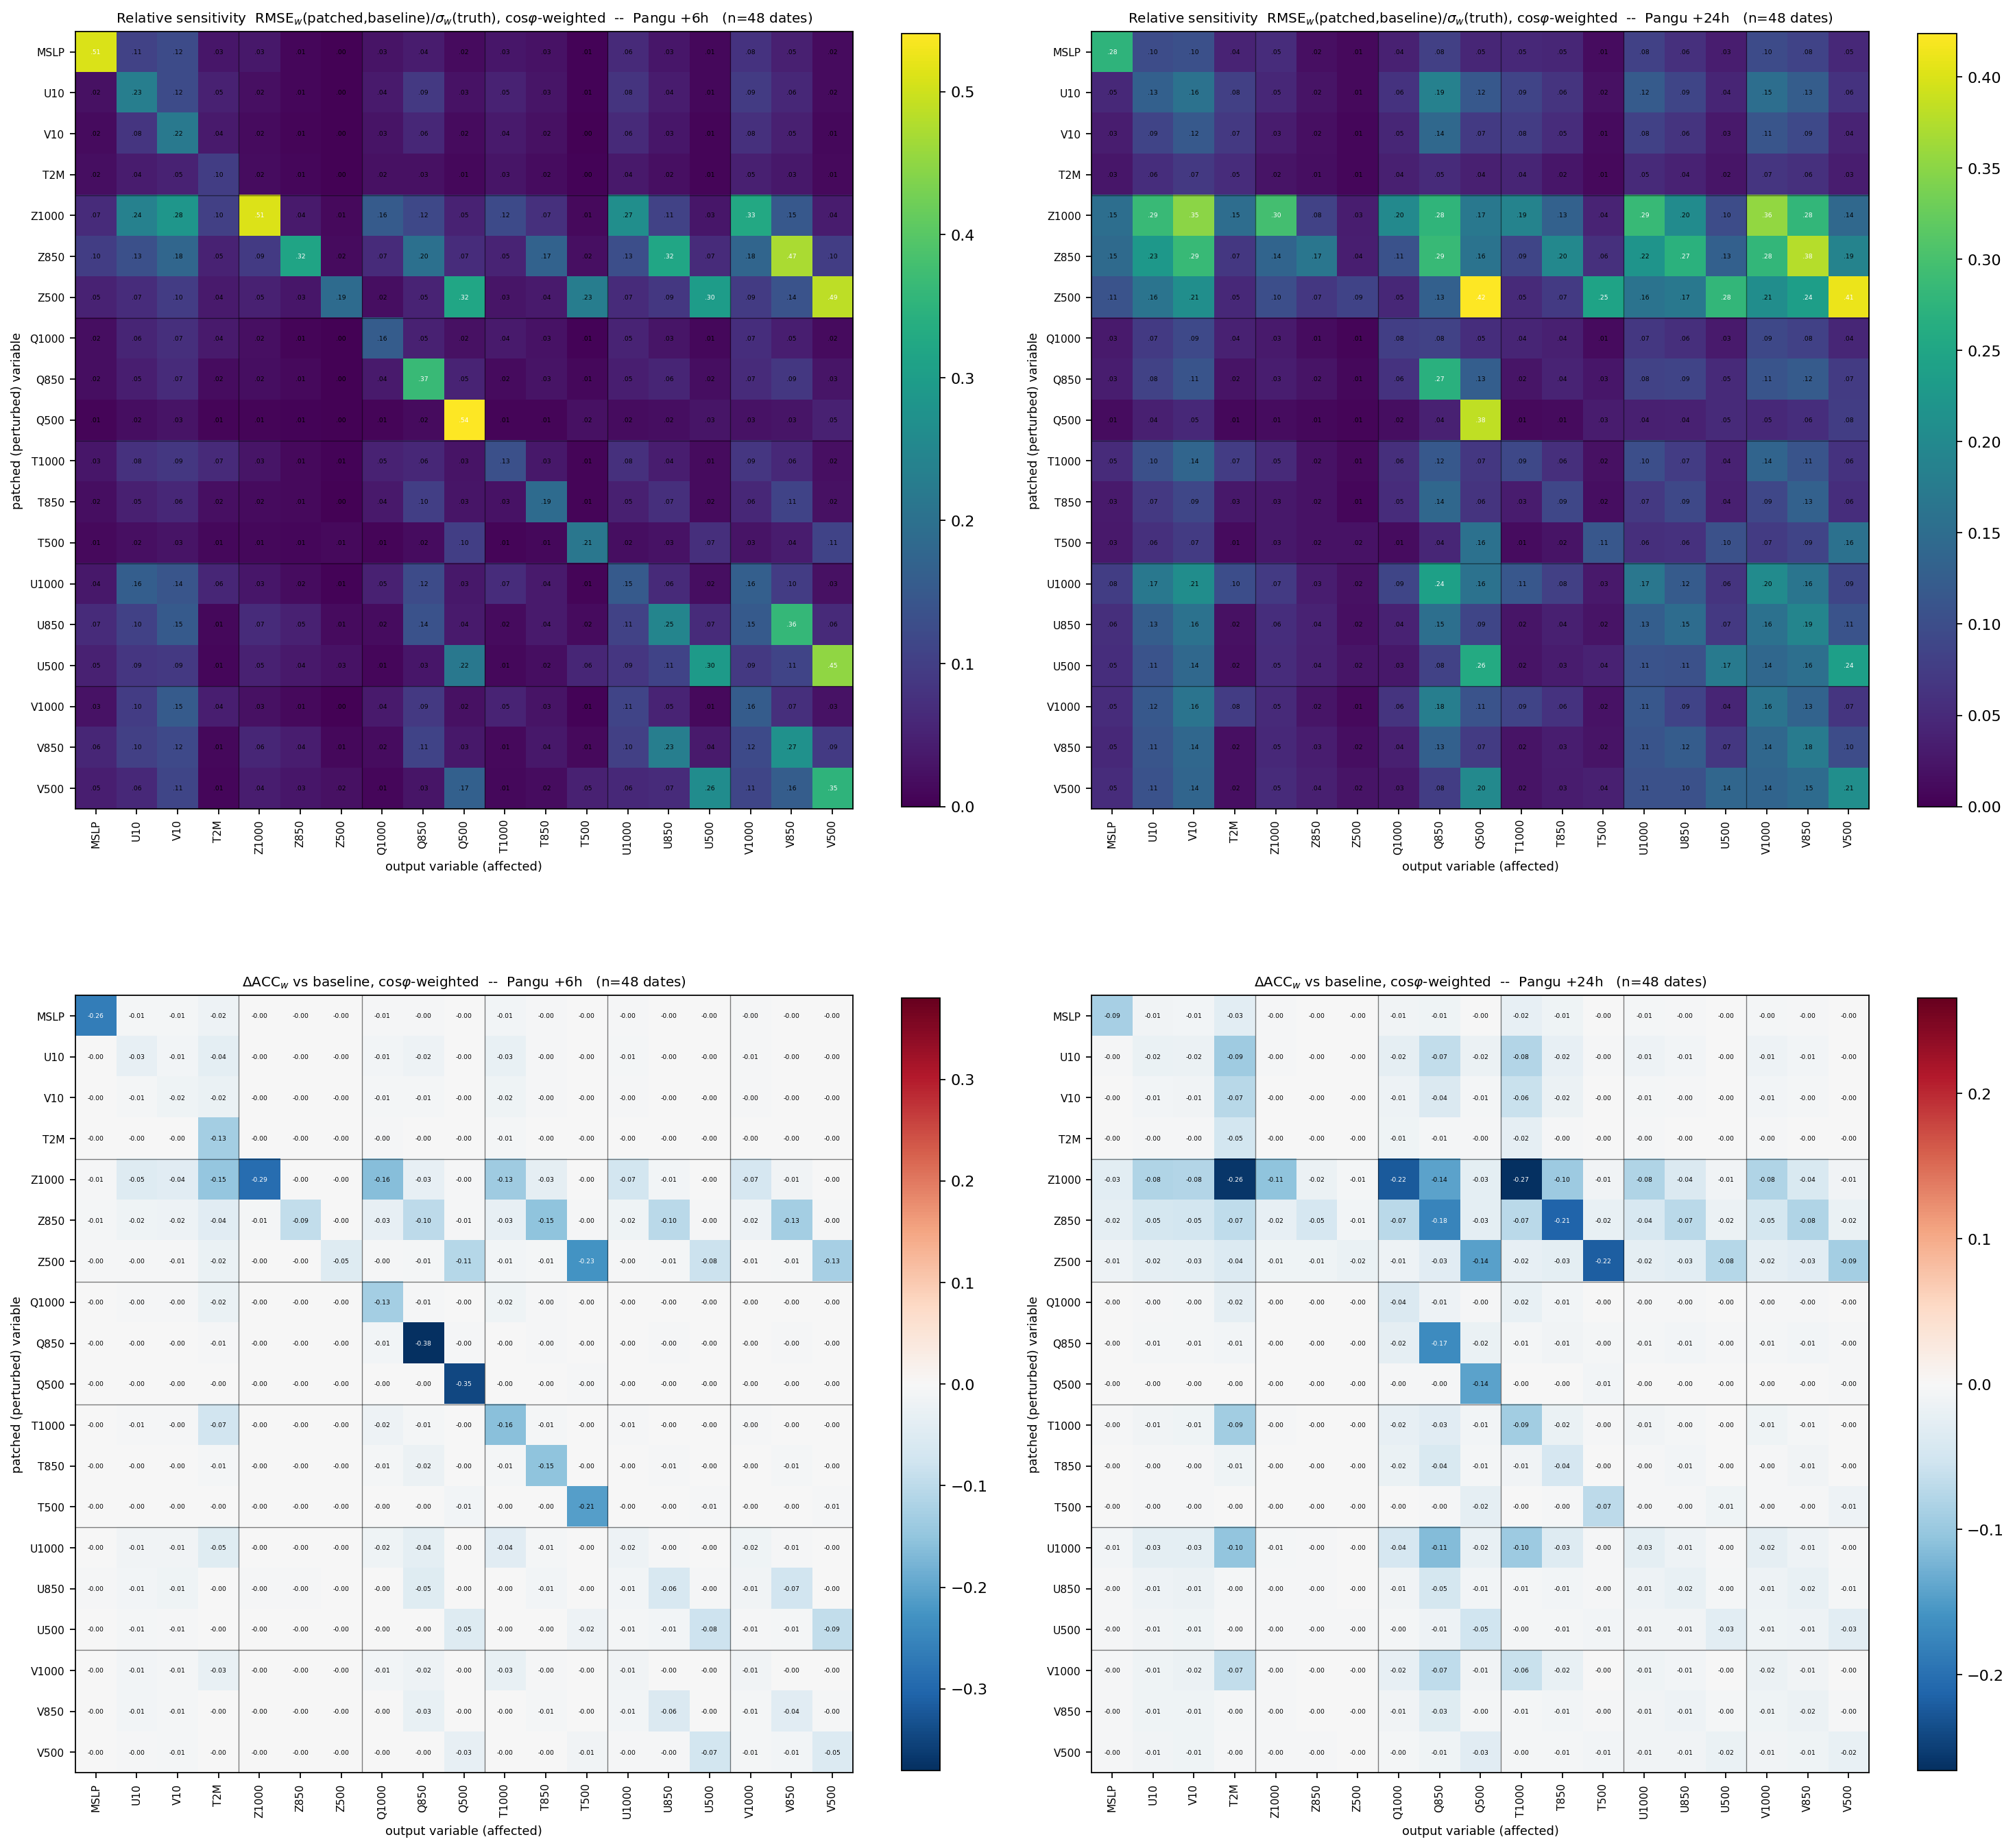
\includegraphics[width=\linewidth,trim=0.30in 8.65in 10.35in 0.12in,clip]{../../figures/patching_matrices/matrix_19var_pangu_n48_weighted.png}
  \\(b) Pangu-Weather, +6 ч
\end{minipage}
\caption{Взвешенная по площади направленная чувствительность $S_{vu}$ для обеих моделей: строка соответствует замененному входу, столбец затронутому выходу. Цветовые шкалы подбираются отдельно, поэтому модели следует сравнивать по числам в ячейках. Полные панели $S$ и $\Delta\acc$ для +6/+24 ч приведены в приложении~\ref{app:figures}.}
\label{fig:matrixoverview}
\end{figure}

\subsection{Направленные матрицы выявляют асимметрию и избыточность}

Корреляция внедиагональных элементов Aurora и Pangu равна $r=0.913$, но сами матрицы несимметричны (рис.~\ref{fig:matrixoverview}). На +6 ч $S_{Z850,V850}$ равен $0.38$ для Aurora и $0.47$ для Pangu; обратные элементы равны $0.04$ и $0.05$. Примерно девятикратный контраст воспроизводится в обеих архитектурах. Диагональ показывает, насколько поле восстанавливается из контекста. У Aurora $S_{Z500,Z500}=0.08$, а $S_{\mathrm{MSLP},\mathrm{MSLP}}=0.45$; у Pangu соответствующие значения равны $0.19$ и $0.53$. Геопотенциал $Z500$ избыточнее, чем MSLP, особенно для Aurora.

\begin{table}[t]
\caption{Основные результаты, среднее по 48 датам. В репозитории сохранены точечные оценки без date-block доверительных интервалов.}
\label{tab:results}
\centering
\small
\begin{tabularx}{\linewidth}{@{}p{0.27\linewidth}Y Y@{}}
\toprule
Диагностика & Численный результат & Интерпретация \\
\midrule
Структура моделей & внедиагональное $r=0.913$ & многие зависимости повторяются в двух архитектурах \\
Направление на +6 ч & $Z850\!\to V850$: $0.38/0.47$; обратно: $0.04/0.05$ (Aurora/Pangu) & связь массового поля с ветром примерно в девять раз сильнее \\
Диагональ на +6 ч & $Z500$: $0.08/0.19$; MSLP: $0.45/0.53$ & MSLP хуже восстанавливается из контекста \\
Наклон дозы $T1000$ & Aurora: $0.690\to0.217$; Pangu: $0.406\to0.614$ (+6$\to$+24 ч) & зависимость от заблаговременности различается \\
Пространственная RMSE $T1000$ & Aurora: $6.02\times/2.01\times$; Pangu: $3.35\times/3.06\times$ (+6/+24 ч) & рост покрывает 99--100\% узлов \\
\bottomrule
\end{tabularx}
\end{table}

\subsection{Доза различает модели}

Все шесть точек дозы $Z1000$ растут без плато до $\alpha=1$. Для Aurora на +6 ч наклоны равны $0.690$ для $T1000$, $0.274$ для $Q1000$ и $0.180/0.187$ для $U/V1000$. Наклон $T1000$ снижается до $0.217$ на +24 ч. У Pangu зависимость от срока другая: наклон $T1000$ растет с $0.406$ до $0.614$, а $T2M$ с $0.387$ до $0.570$. Полная замена ранжирует конечную чувствительность модели; промежуточные точки показывают, почему ее нельзя трактовать как инфинитезимальный якобиан.

\subsection{Пространственный отклик сохраняется на большей части сетки}

Композит $T1000$ на рис.~\ref{fig:bias} показывает временную RMSE в каждом узле, патченный прогноз минус базовый. На +6 ч полная замена $Z1000$ увеличивает среднюю по узлам RMSE $T1000$ в $6.02$ раза у Aurora и в $3.35$ раза у Pangu. На +24 ч отношения равны $2.01$ и $3.06$. Рост охватывает 99--100\% узлов. У Aurora эффект заметно ослабевает к +24 ч, у Pangu сохраняется почти полностью. В обеих моделях крупные приращения сосредоточены в средних и высоких широтах; у Pangu отклик шире в тропиках и субтропиках.

\begin{figure}[t]
\centering
\begin{minipage}[t]{0.485\linewidth}
  \centering
  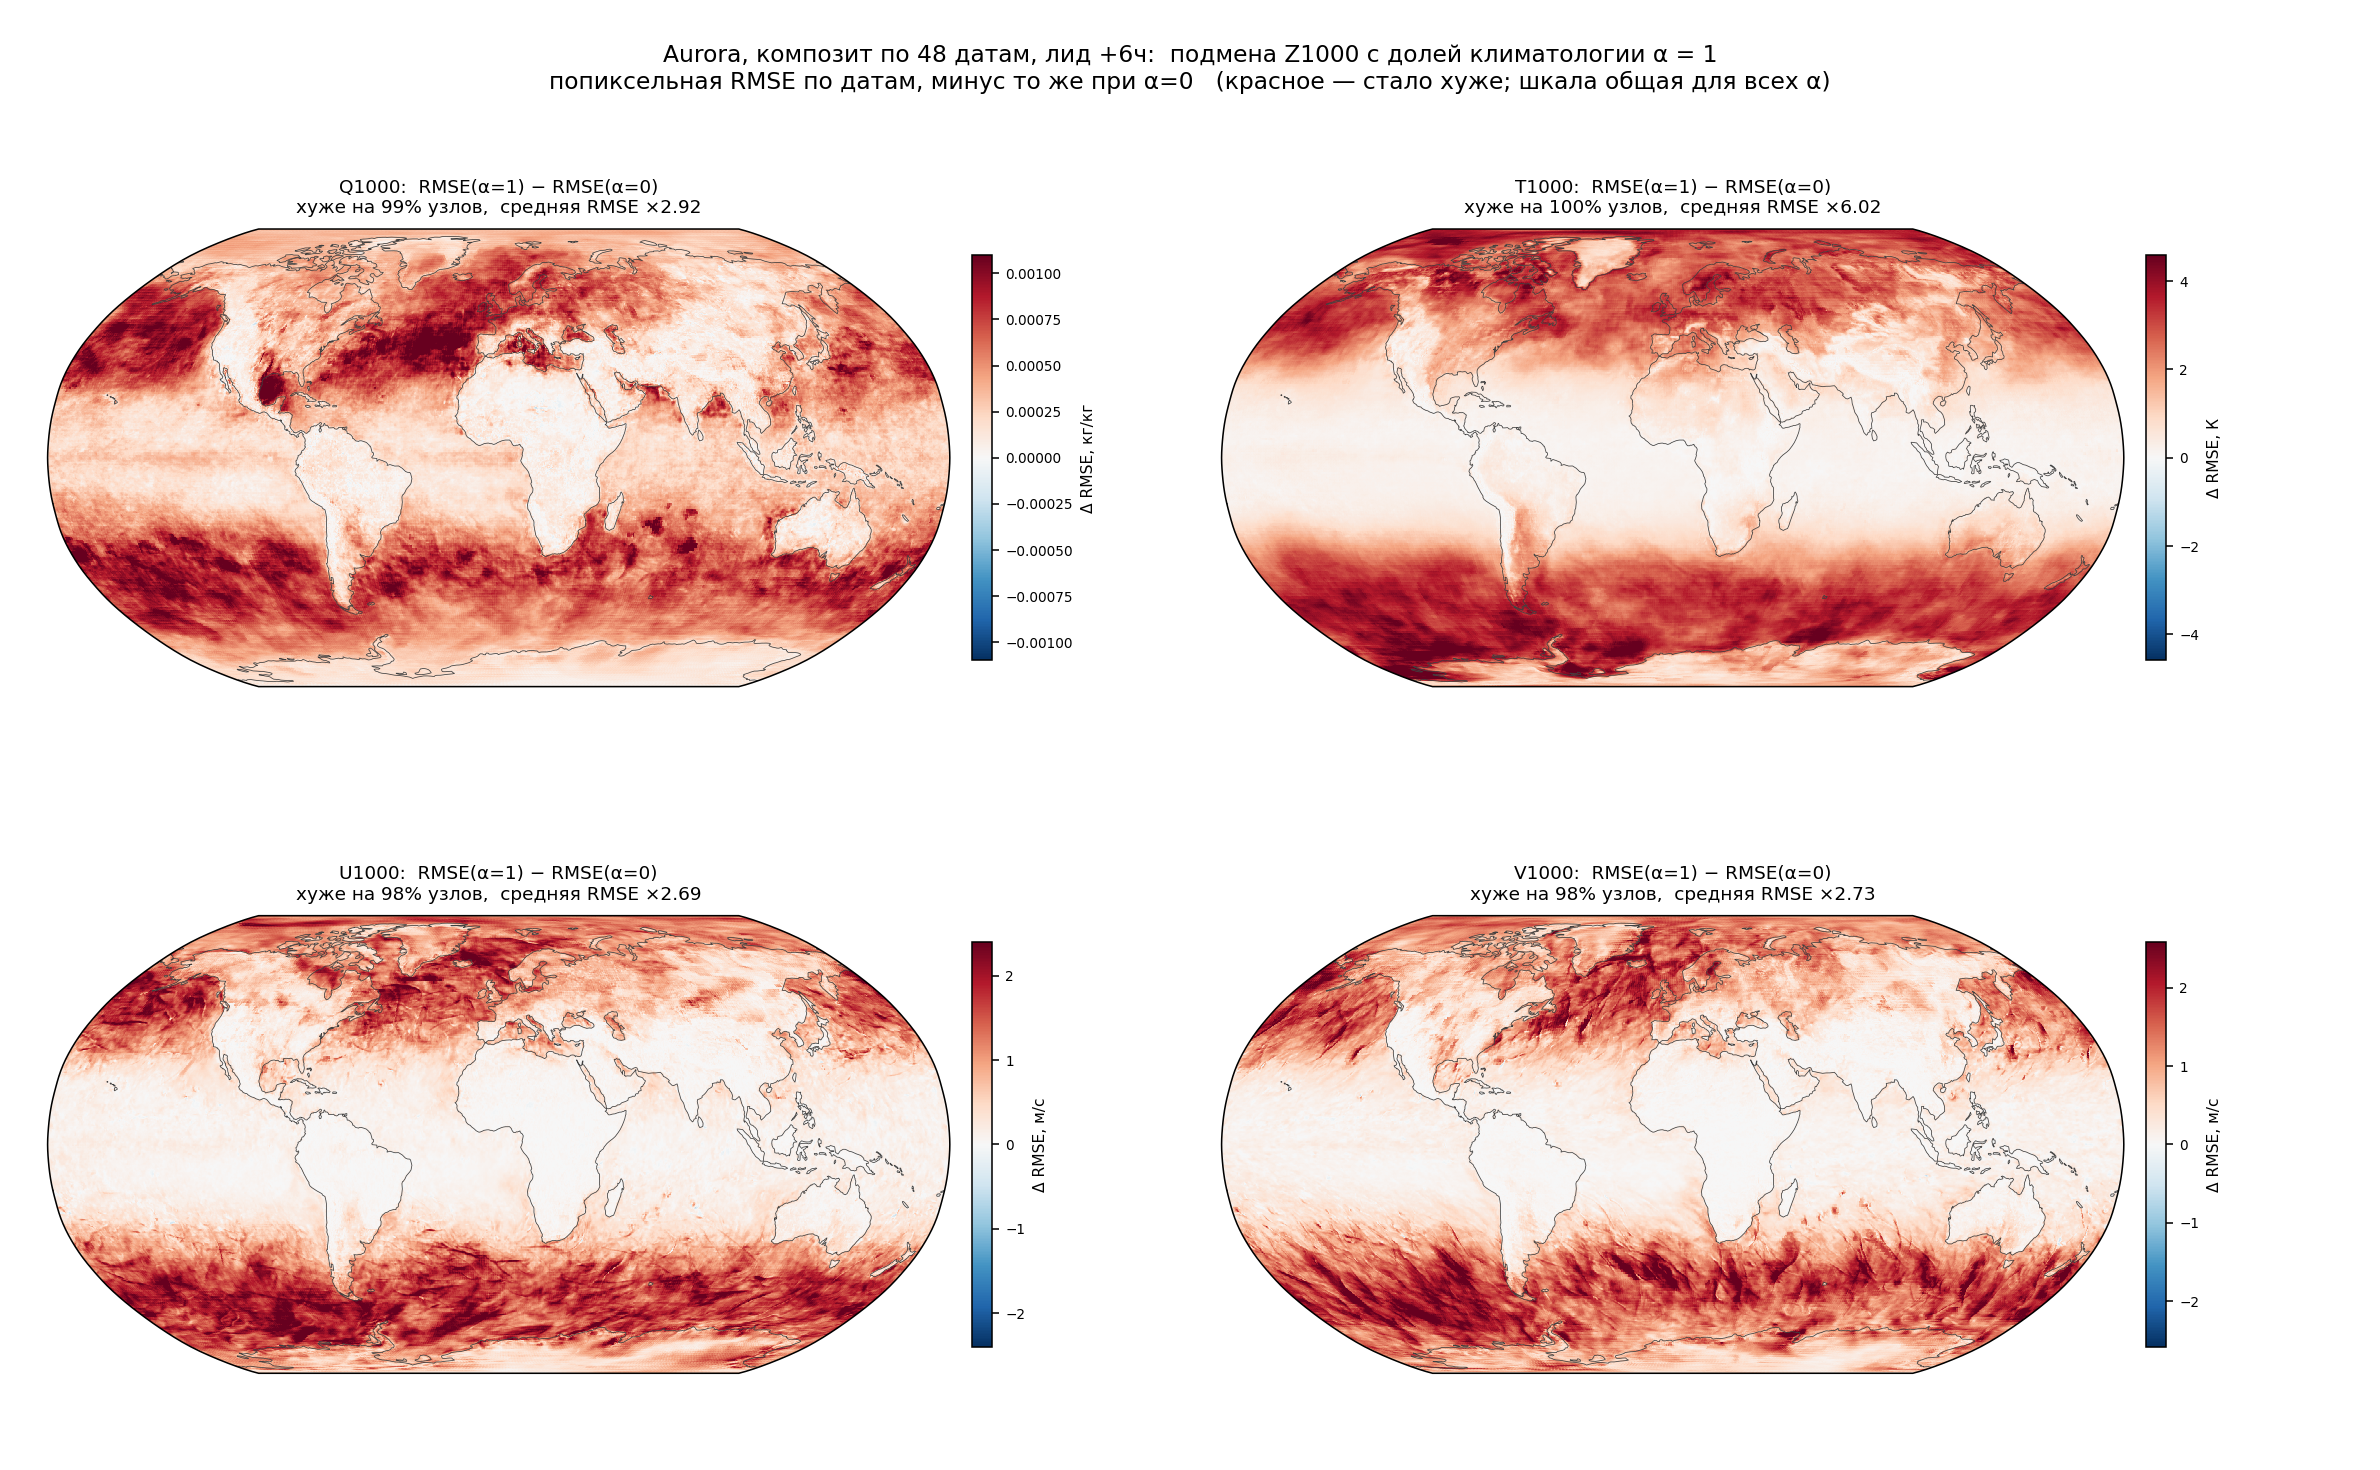
\includegraphics[width=\linewidth,trim=8.10in 5.55in 0.20in 1.58in,clip]{../../figures/bias_maps/composite_bias_Z1000_lead6_alpha1_n48.png}
  \\(a) Aurora, +6 ч: $6.02\times$
\end{minipage}\hfill
\begin{minipage}[t]{0.485\linewidth}
  \centering
  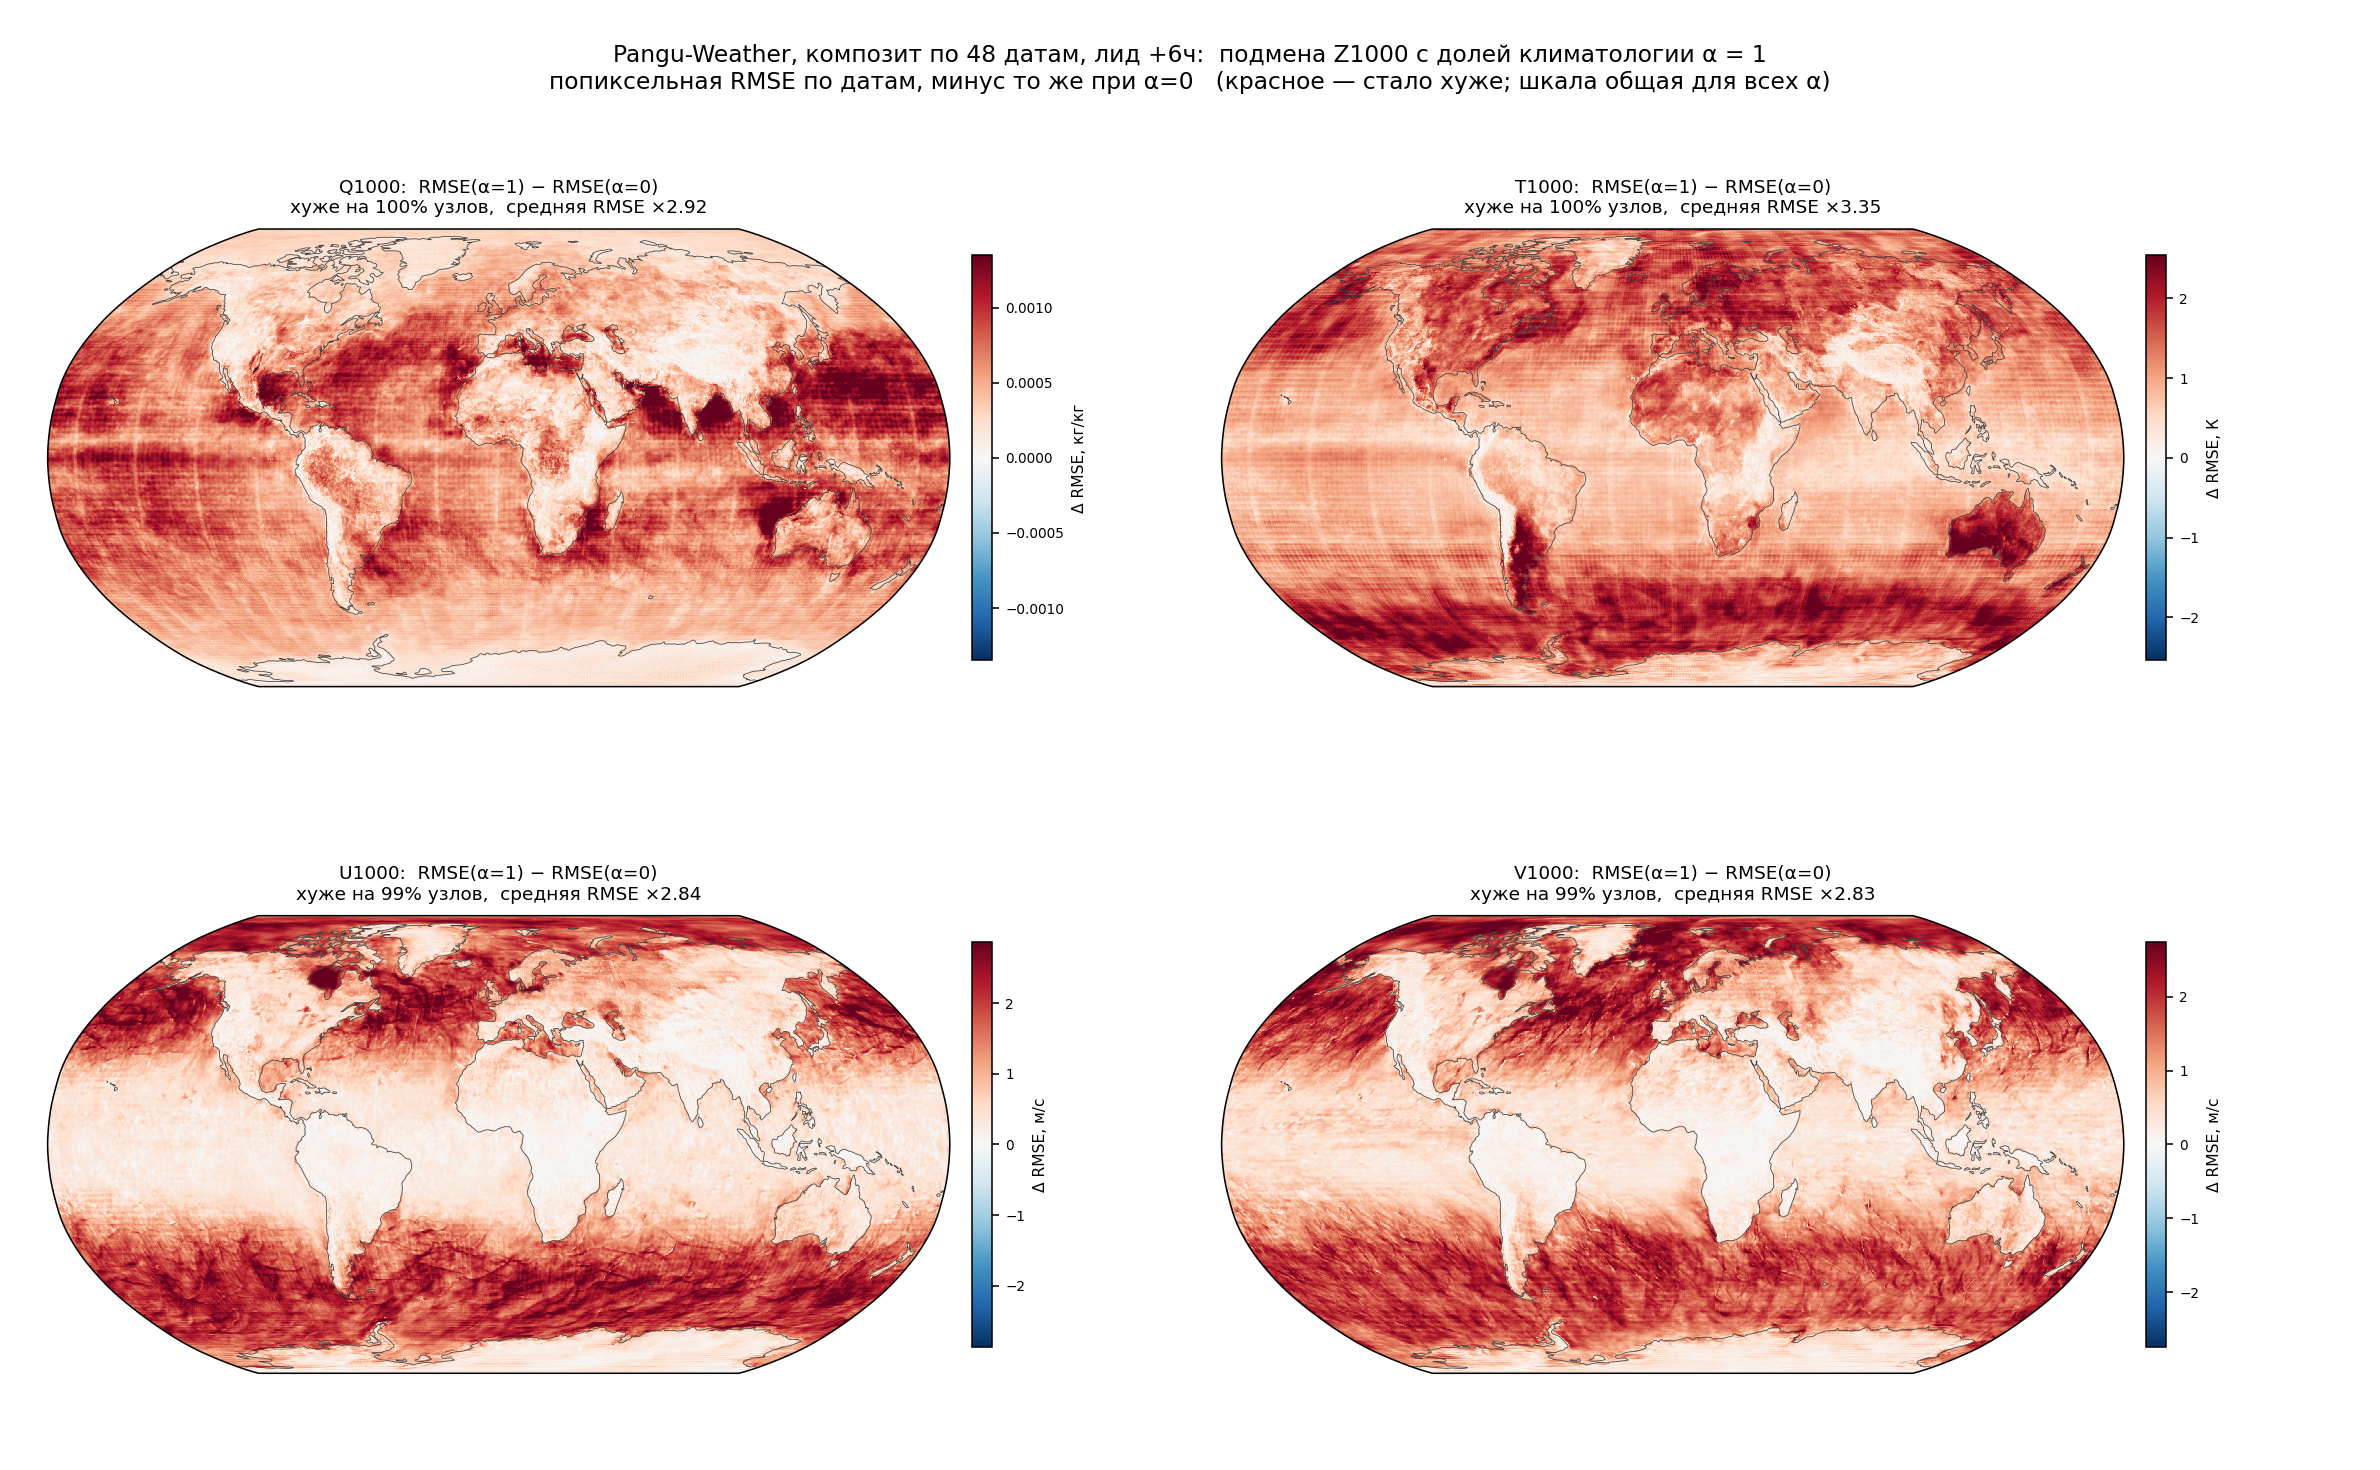
\includegraphics[width=\linewidth,trim=8.10in 5.55in 0.20in 1.58in,clip]{../../figures/bias_maps/composite_bias_pangu_Z1000_lead6_alpha1_n48.png}
  \\(b) Pangu-Weather, +6 ч: $3.35\times$
\end{minipage}

\begin{minipage}[t]{0.485\linewidth}
  \centering
  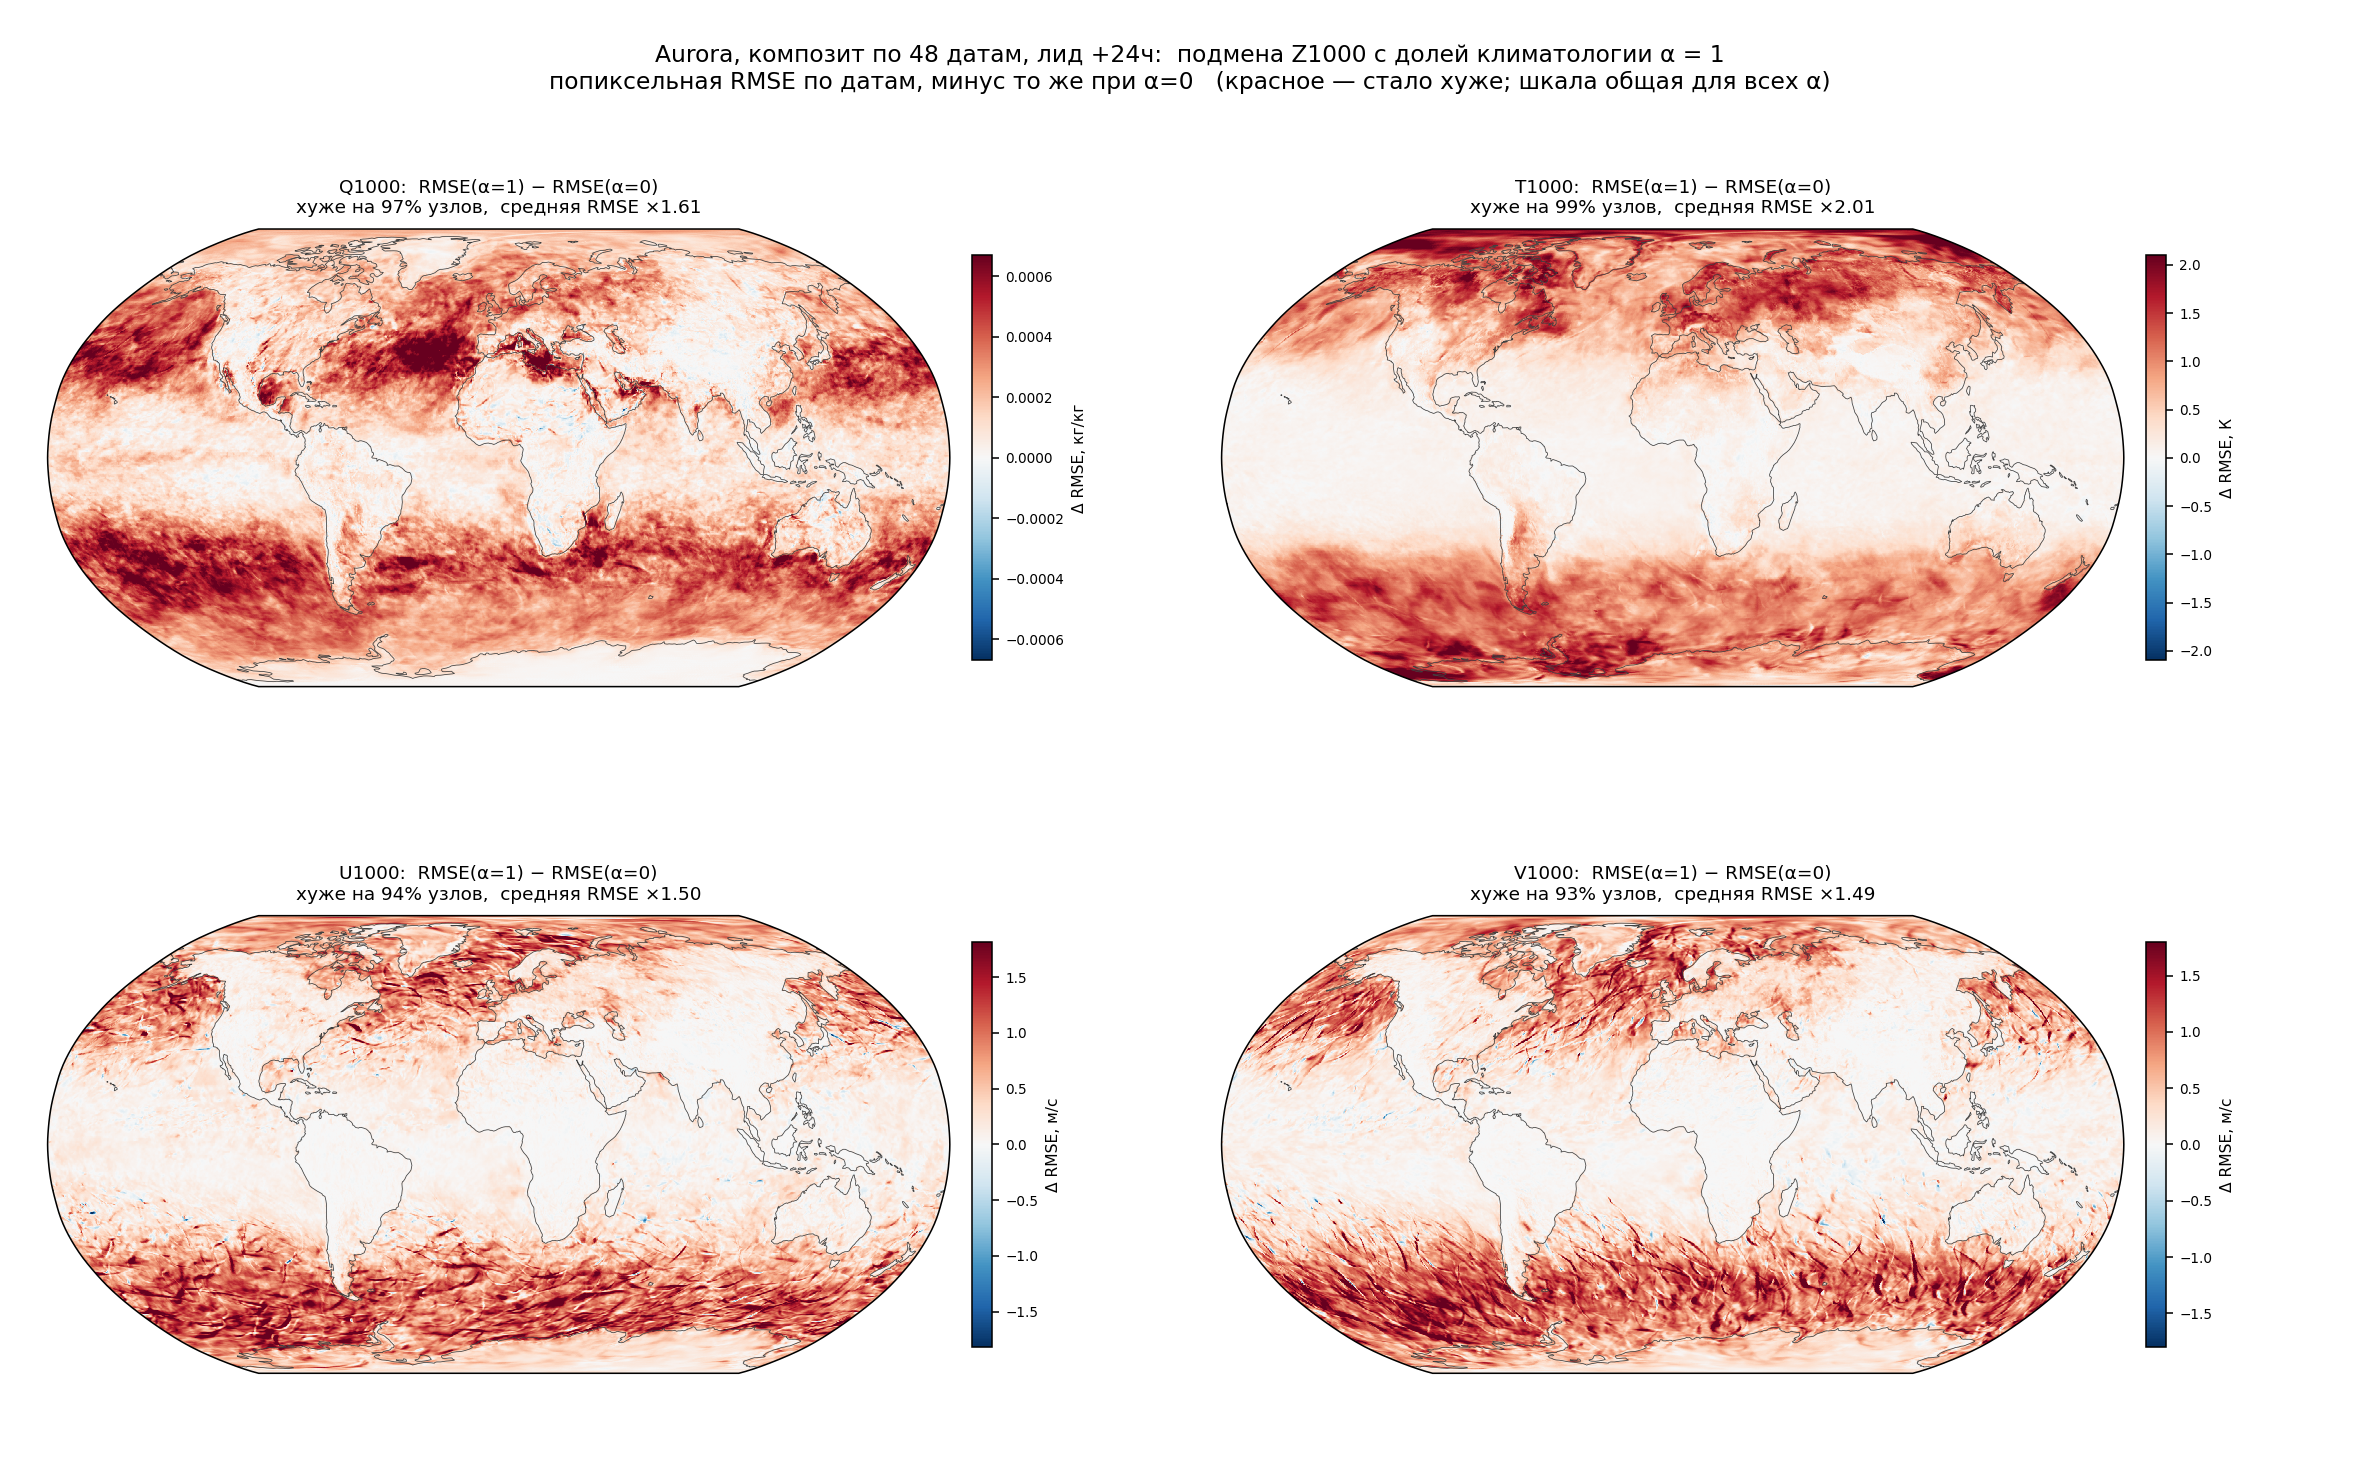
\includegraphics[width=\linewidth,trim=8.10in 5.55in 0.20in 1.58in,clip]{../../figures/bias_maps/composite_bias_Z1000_lead24_alpha1_n48.png}
  \\(c) Aurora, +24 ч: $2.01\times$
\end{minipage}\hfill
\begin{minipage}[t]{0.485\linewidth}
  \centering
  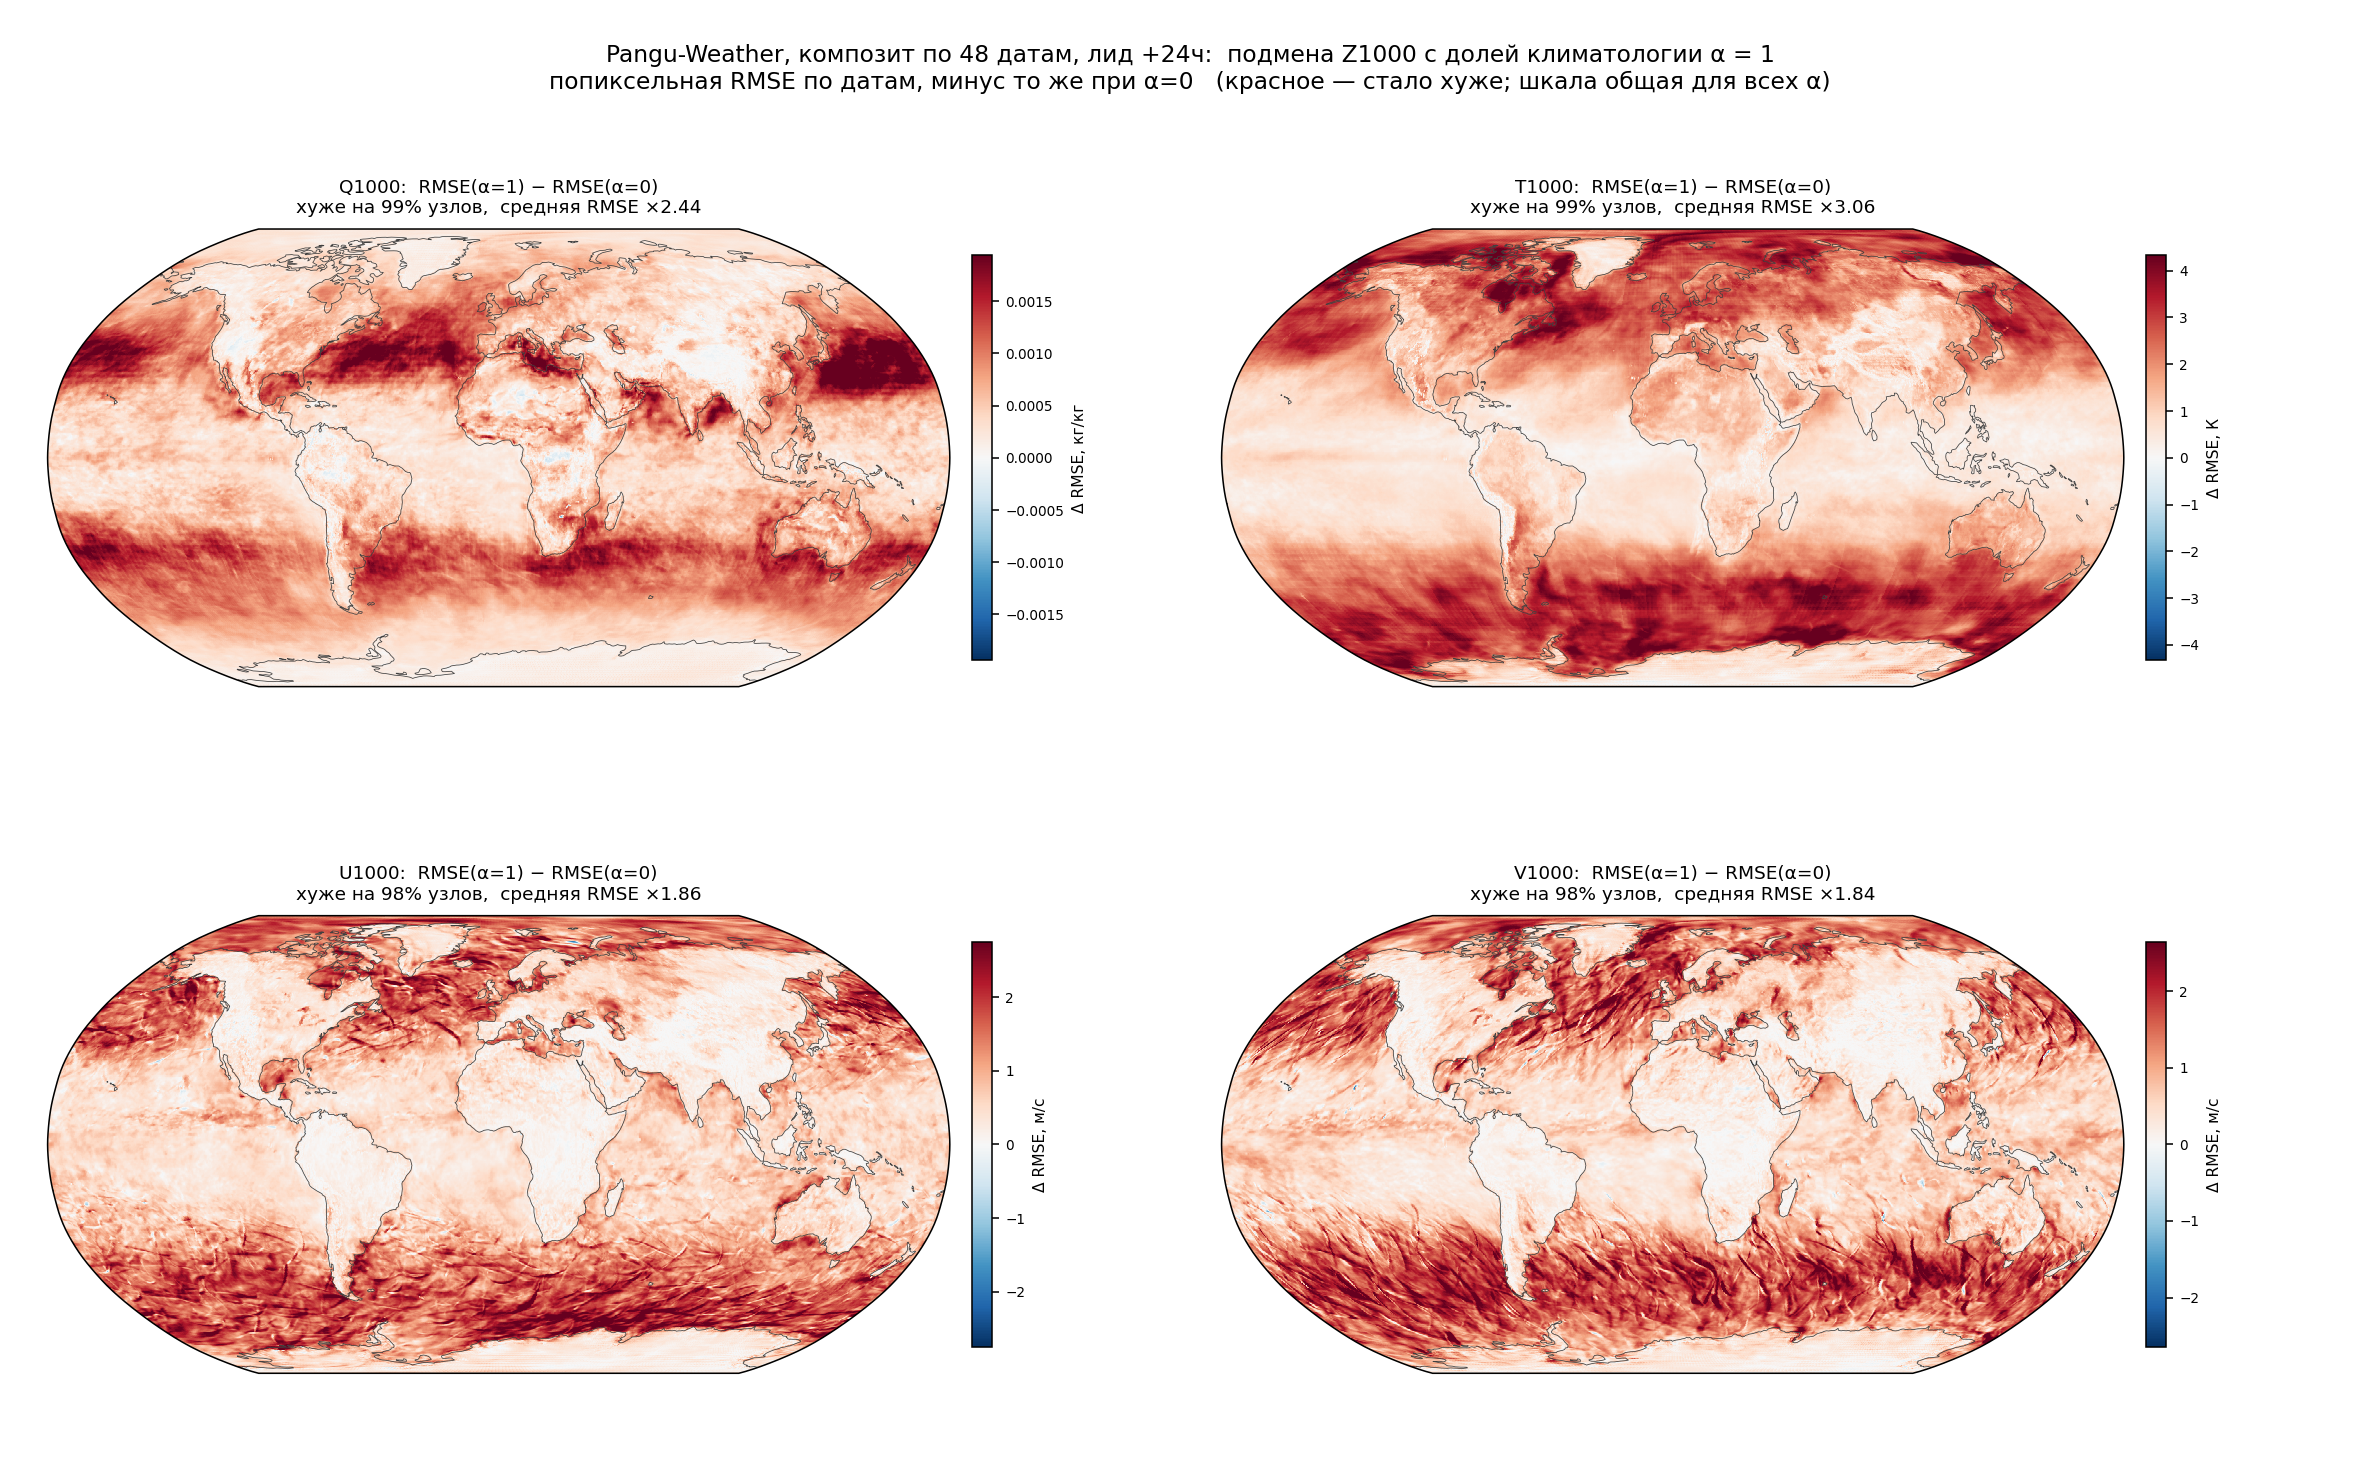
\includegraphics[width=\linewidth,trim=8.10in 5.55in 0.20in 1.58in,clip]{../../figures/bias_maps/composite_bias_pangu_Z1000_lead24_alpha1_n48.png}
  \\(d) Pangu-Weather, +24 ч: $3.06\times$
\end{minipage}
\caption{Изменение временной RMSE $T1000$ в каждом узле после полной замены $Z1000$ ($\alpha=1$). Красный цвет соответствует большей ошибке относительно базового прогноза. В каждой панели сохранена исходная шкала; под картами указано отношение средних по узлам RMSE.}
\label{fig:bias}
\end{figure}

\section{Обсуждение}

Связь массового поля с ветром и связь толщины слоя с температурой нижней тропосферы согласуются с основной структурой матриц. Интервенция определяет зависимость только внутри обученной сети. Замена полного поля климатологией является крупным, частично out-of-distribution изменением; корреляции одного момента дополнительно смешивают географию, сезон и динамику.

Оценка охватывает 48 дат одного года, две короткие заблаговременности и три изобарических уровня. Ансамбли и date-block bootstrap интервалы отсутствуют. Исходные массивы лежат во внешнем кластерном хранилище, которое было недоступно при подготовке статьи, поэтому числа проверены по сохраненным рисункам, подписям и коду анализа без повторного расчета. Для операционной оценки нужны интервалы неопределенности, стратификация событий, более длинные прогнозы и данные, доступные на момент выпуска прогноза.

\paragraph{Климатическая значимость и риски.} Разработчики могут применять аудит для поиска хрупкой зависимости от каналов до включения модели в систему раннего предупреждения или климатический сервис. Аудит не повышает точность прогноза, не оценивает антропогенное изменение климата и не валидирует правило принятия решений. Его следует использовать вместе со стандартными метриками, калибровкой и экспертной оценкой. Следующий эксперимент должен повторить парные интервенции для разных событий и сроков, рассчитать date-block интервалы и использовать данные, доступные на момент выпуска прогноза.

\clearpage
\bibliographystyle{unsrt}
\bibliography{references}

\clearpage
\appendix
\section{Полноразмерные результаты}
\label{app:figures}

\begin{figure}[ht]
\centering
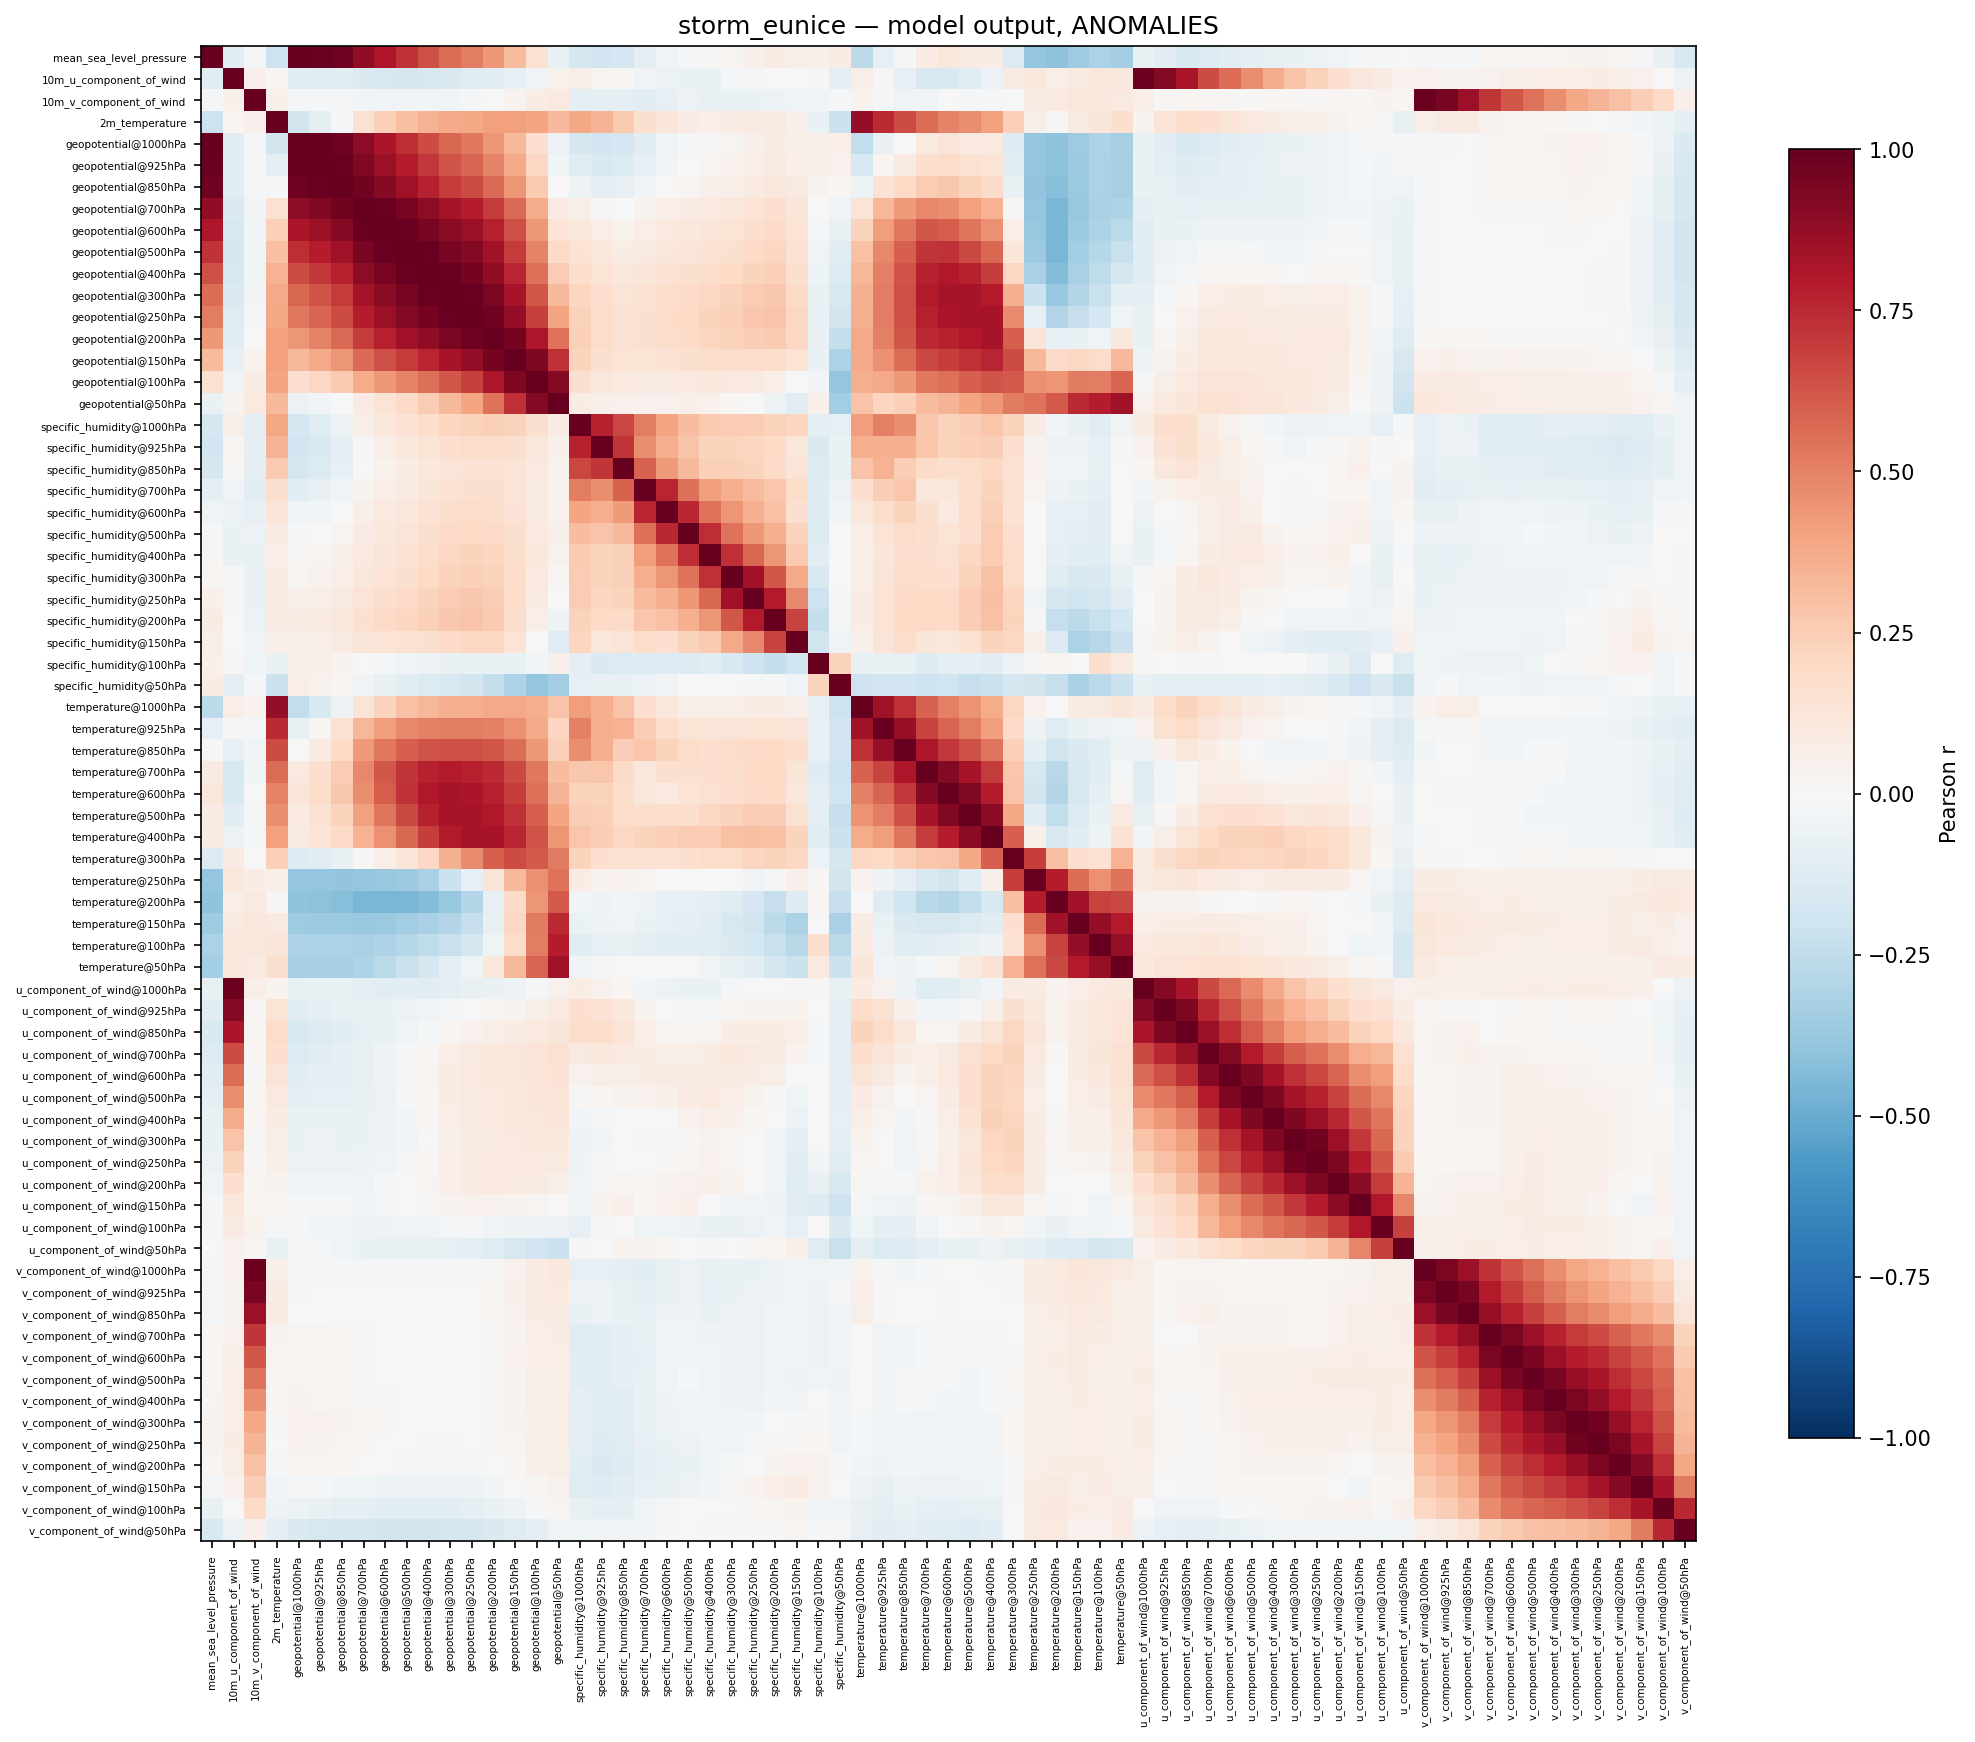
\includegraphics[width=\linewidth]{../../figures/model_comparison/storm_eunice_corr_model_anomaly.png}
\caption{Корреляционная матрица аномалий 69 выходных каналов Pangu-Weather для шторма Eunice. Блочная структура описательна и не имеет направления.}
\end{figure}

\begin{figure}[p]
\centering
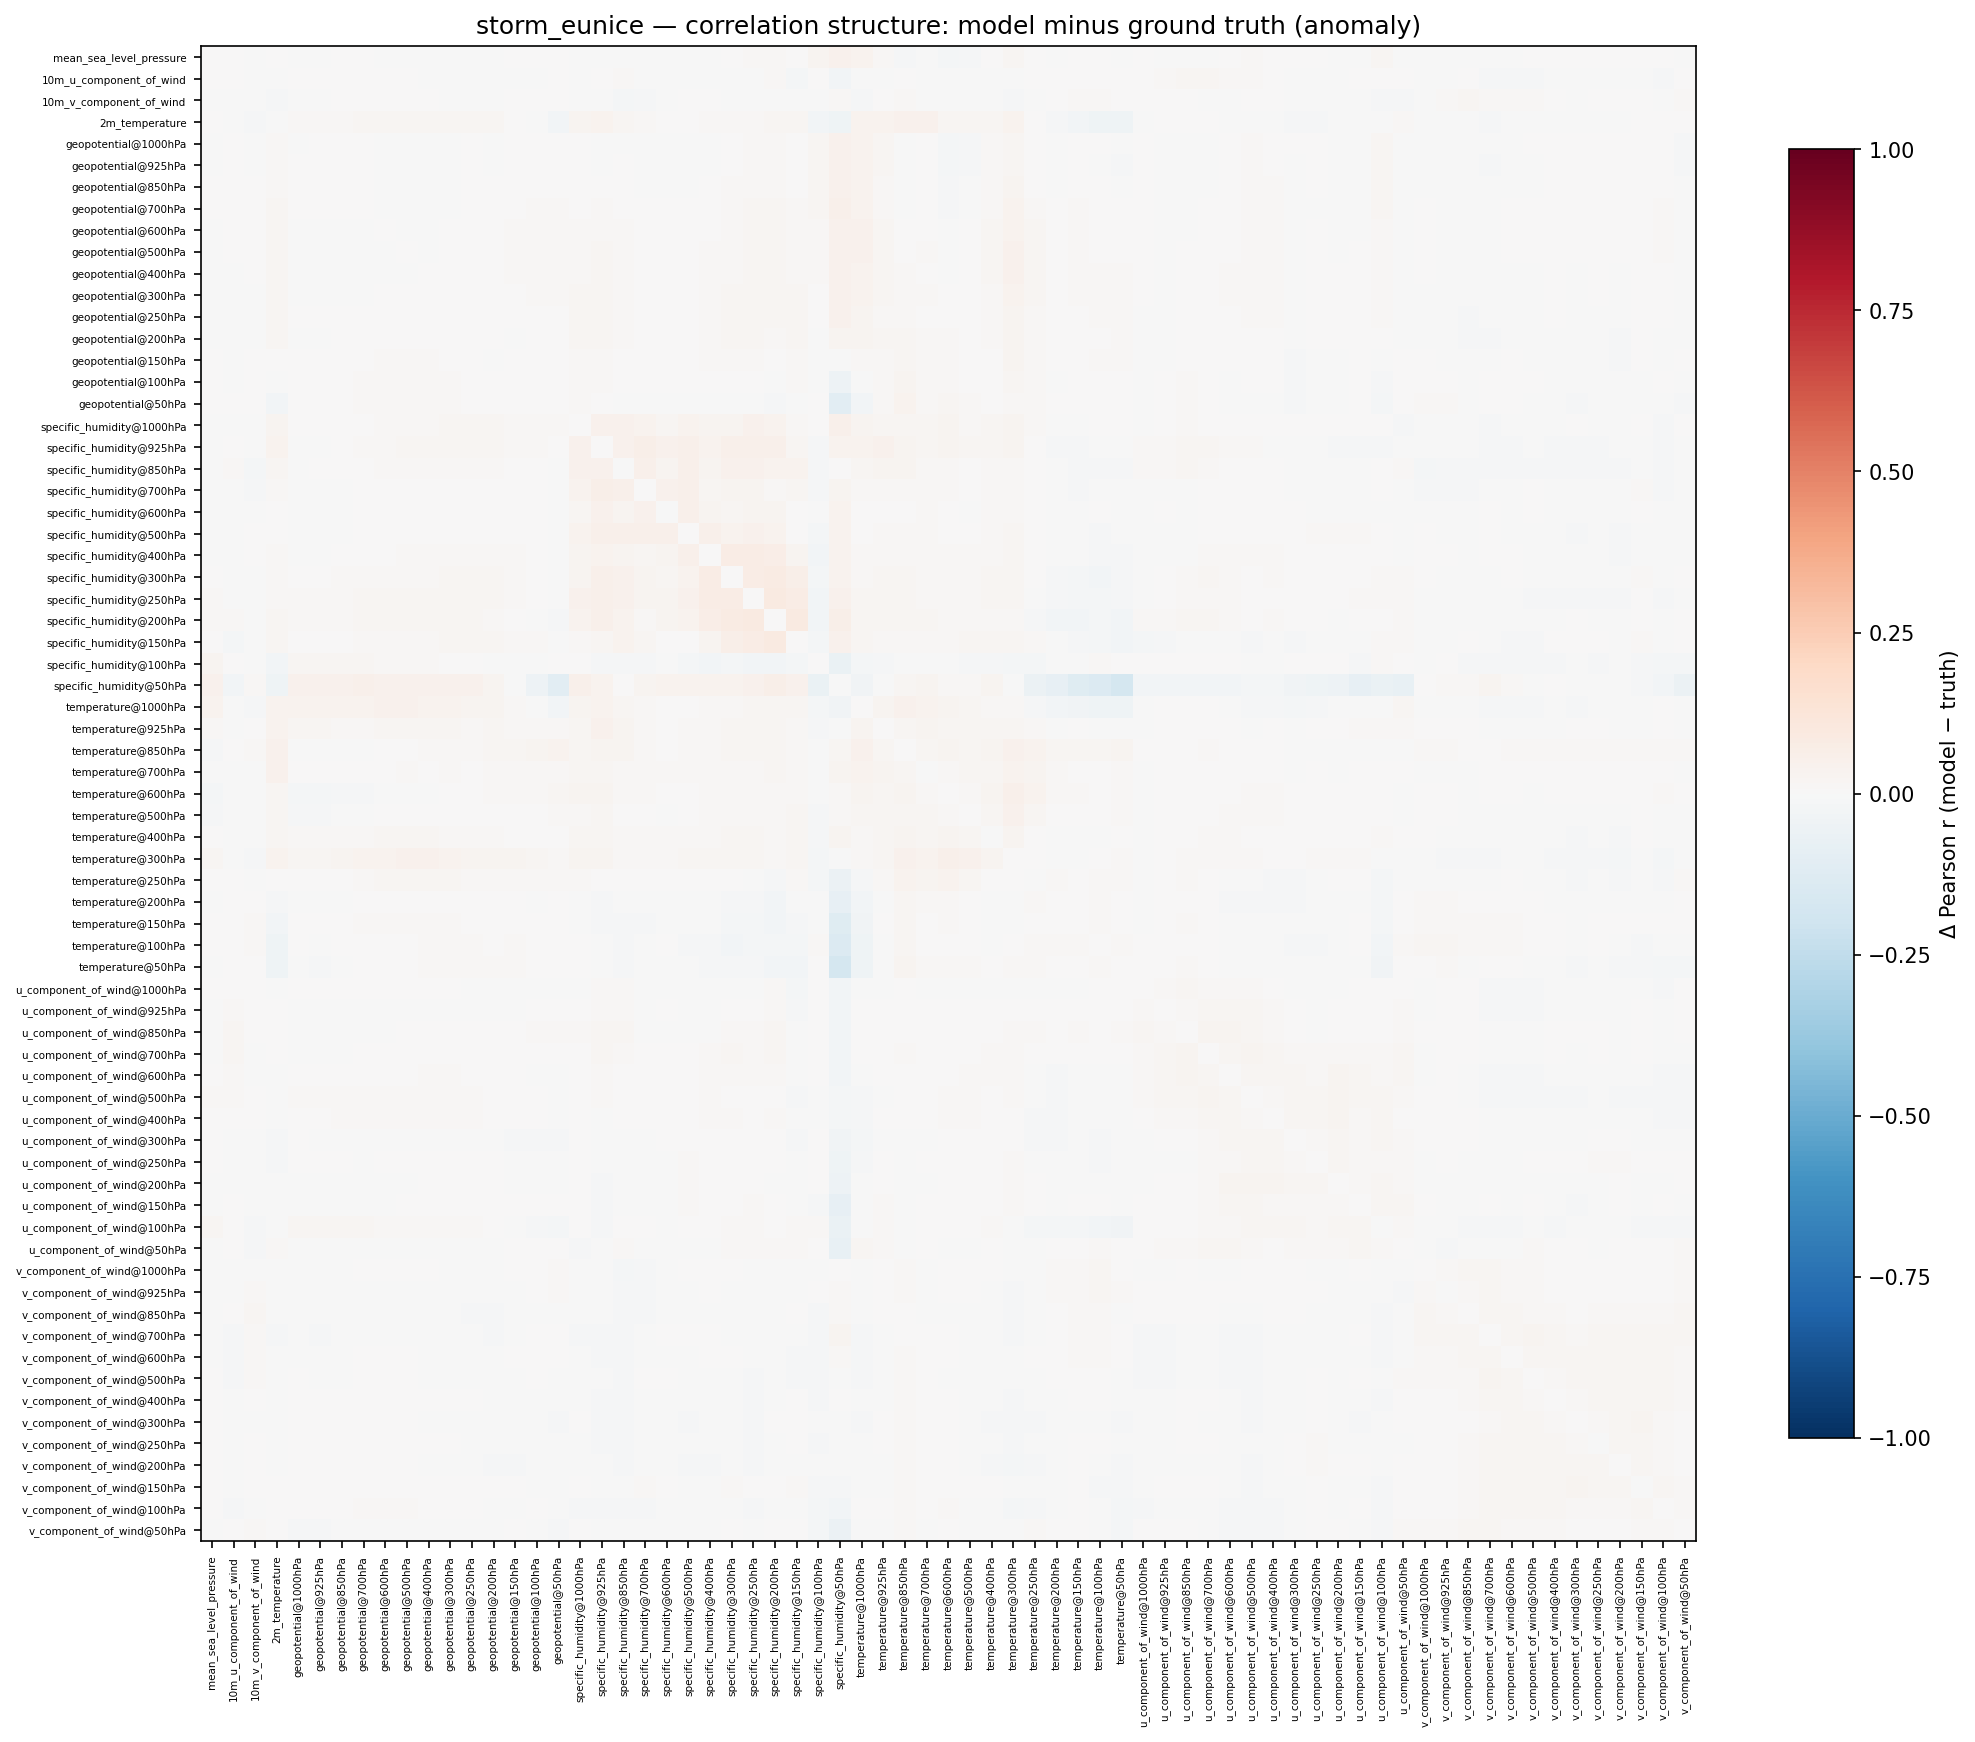
\includegraphics[width=\linewidth]{../../figures/model_comparison/storm_eunice_corr_diff_anomaly.png}
\caption{Разность корреляционной структуры аномалий Pangu-Weather и ERA5 для того же случая.}
\end{figure}

\begin{figure}[p]
\centering
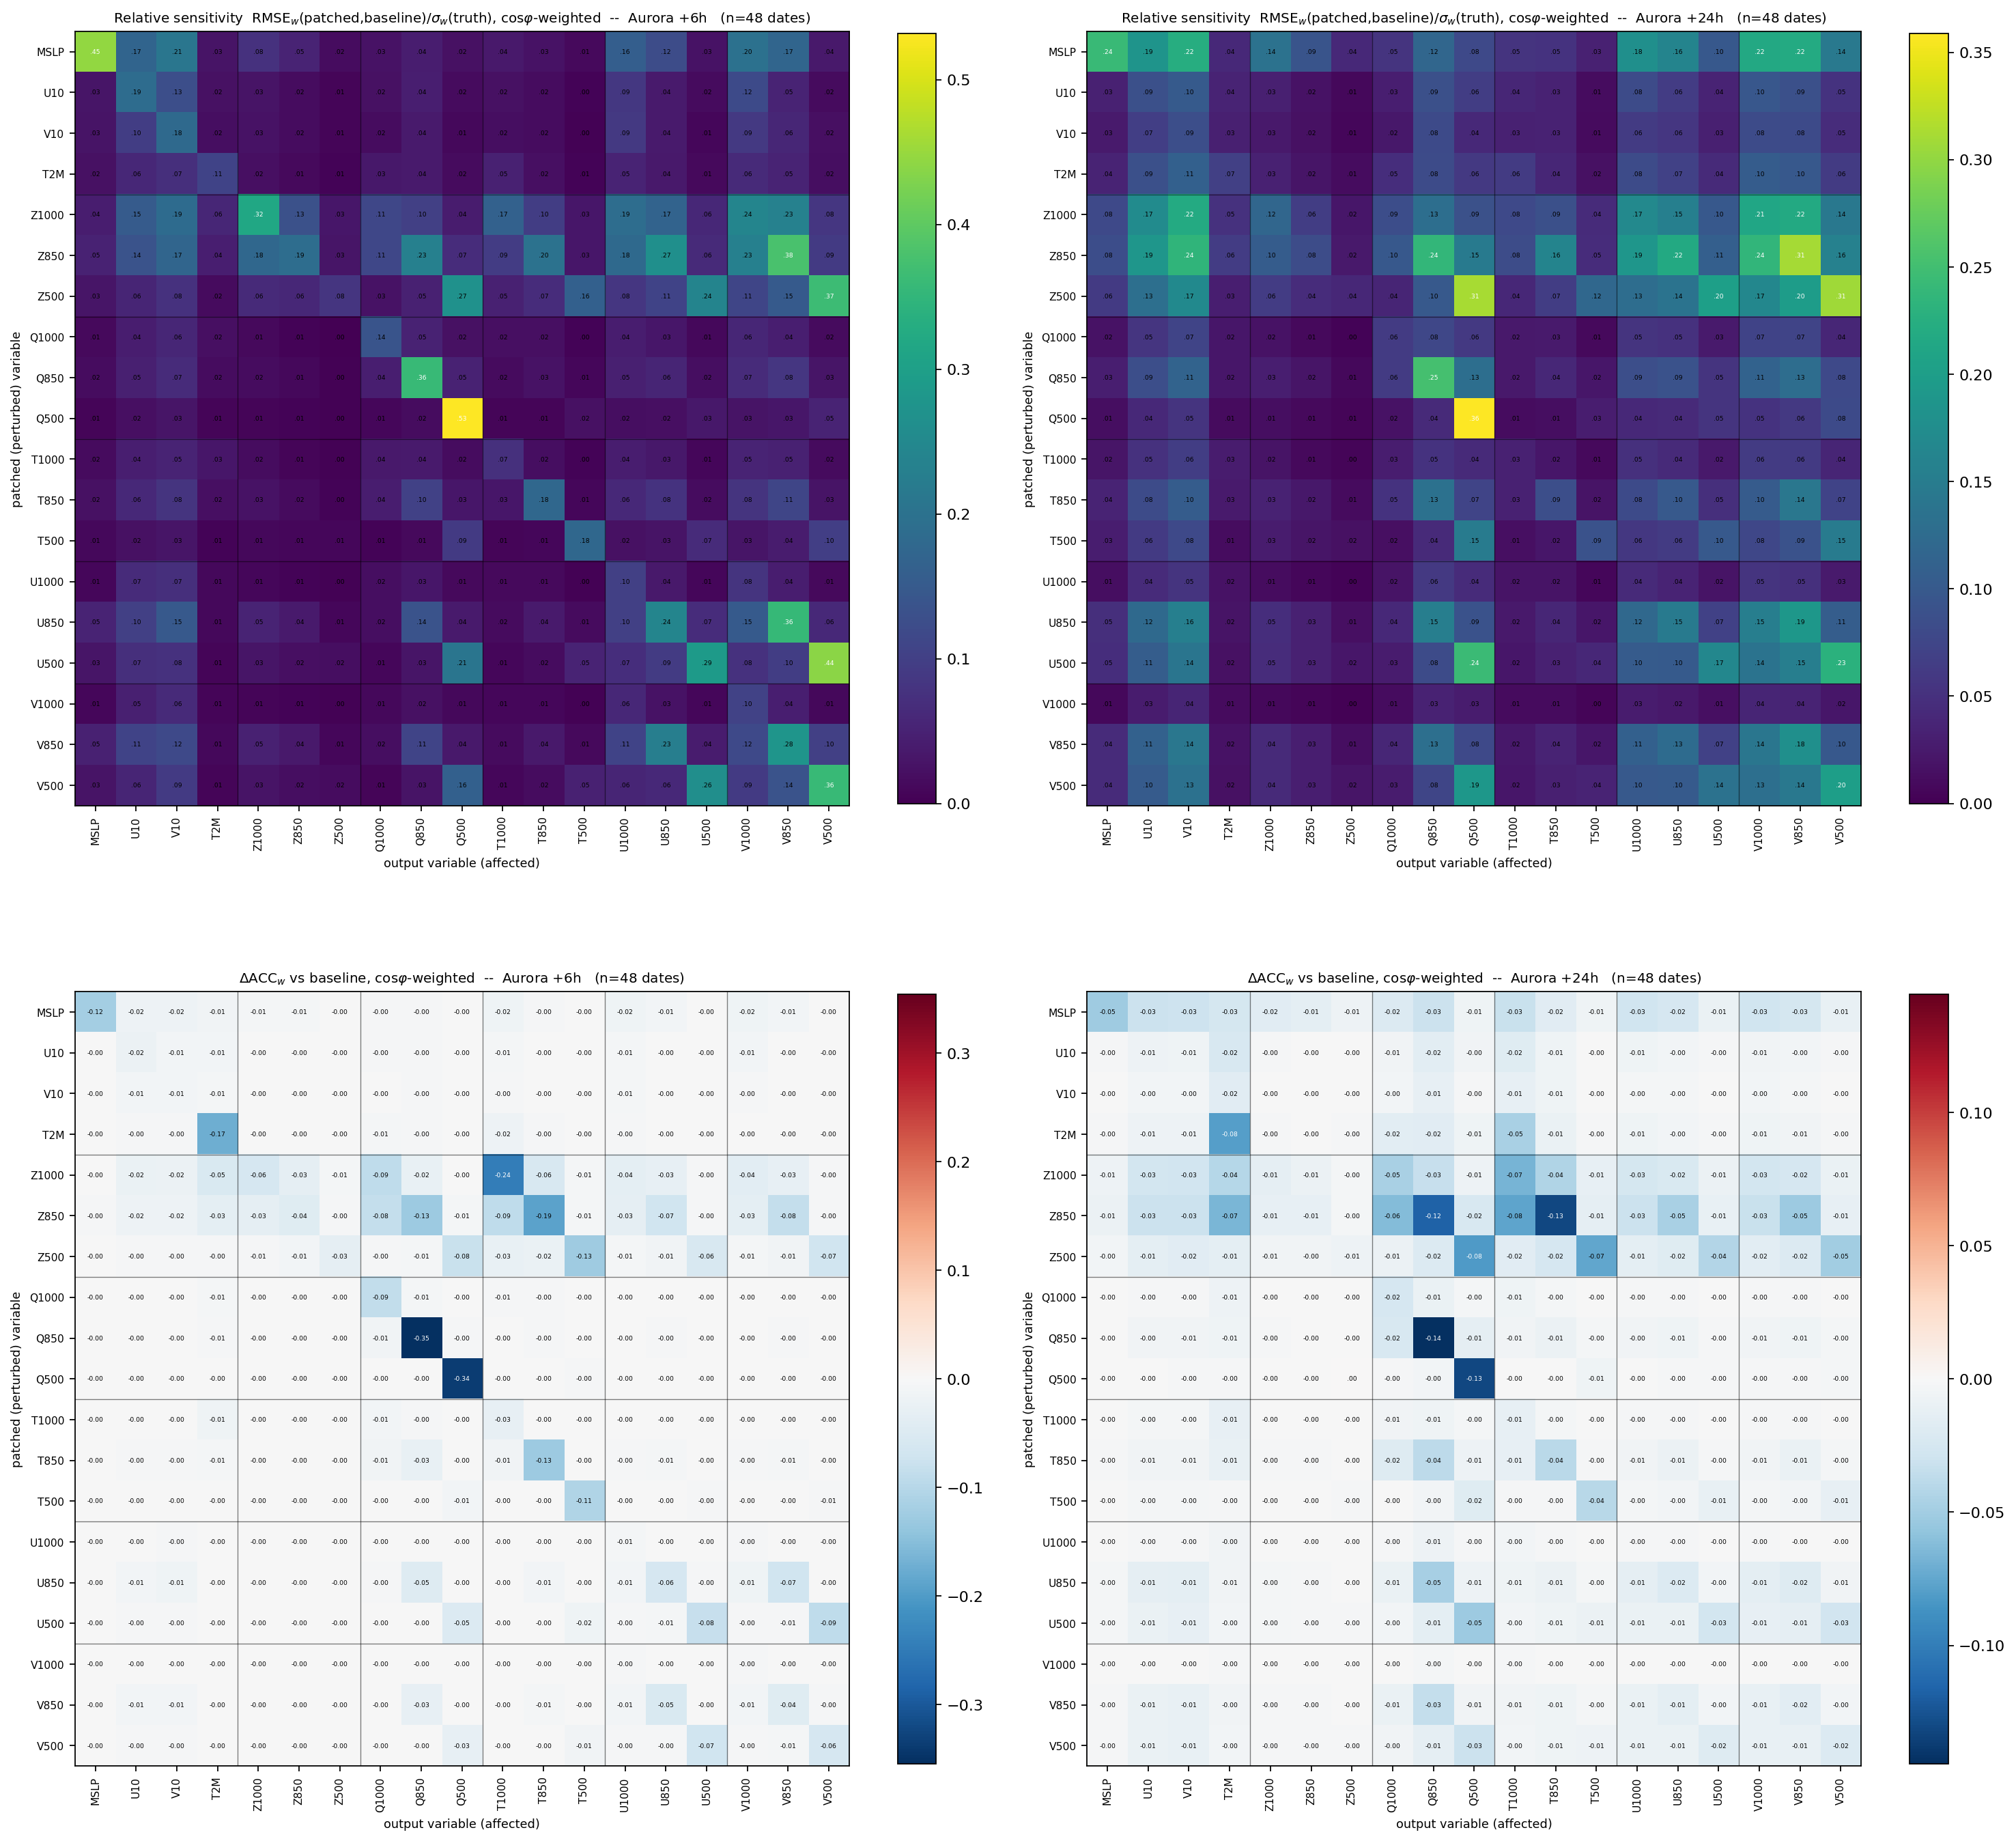
\includegraphics[width=\linewidth]{../../figures/patching_matrices/matrix_19var_aurora_n48_weighted.png}
\caption{Aurora: полные взвешенные по площади матрицы относительной чувствительности и $\Delta$ACC на +6 и +24 ч ($n=48$).}
\end{figure}

\begin{figure}[p]
\centering
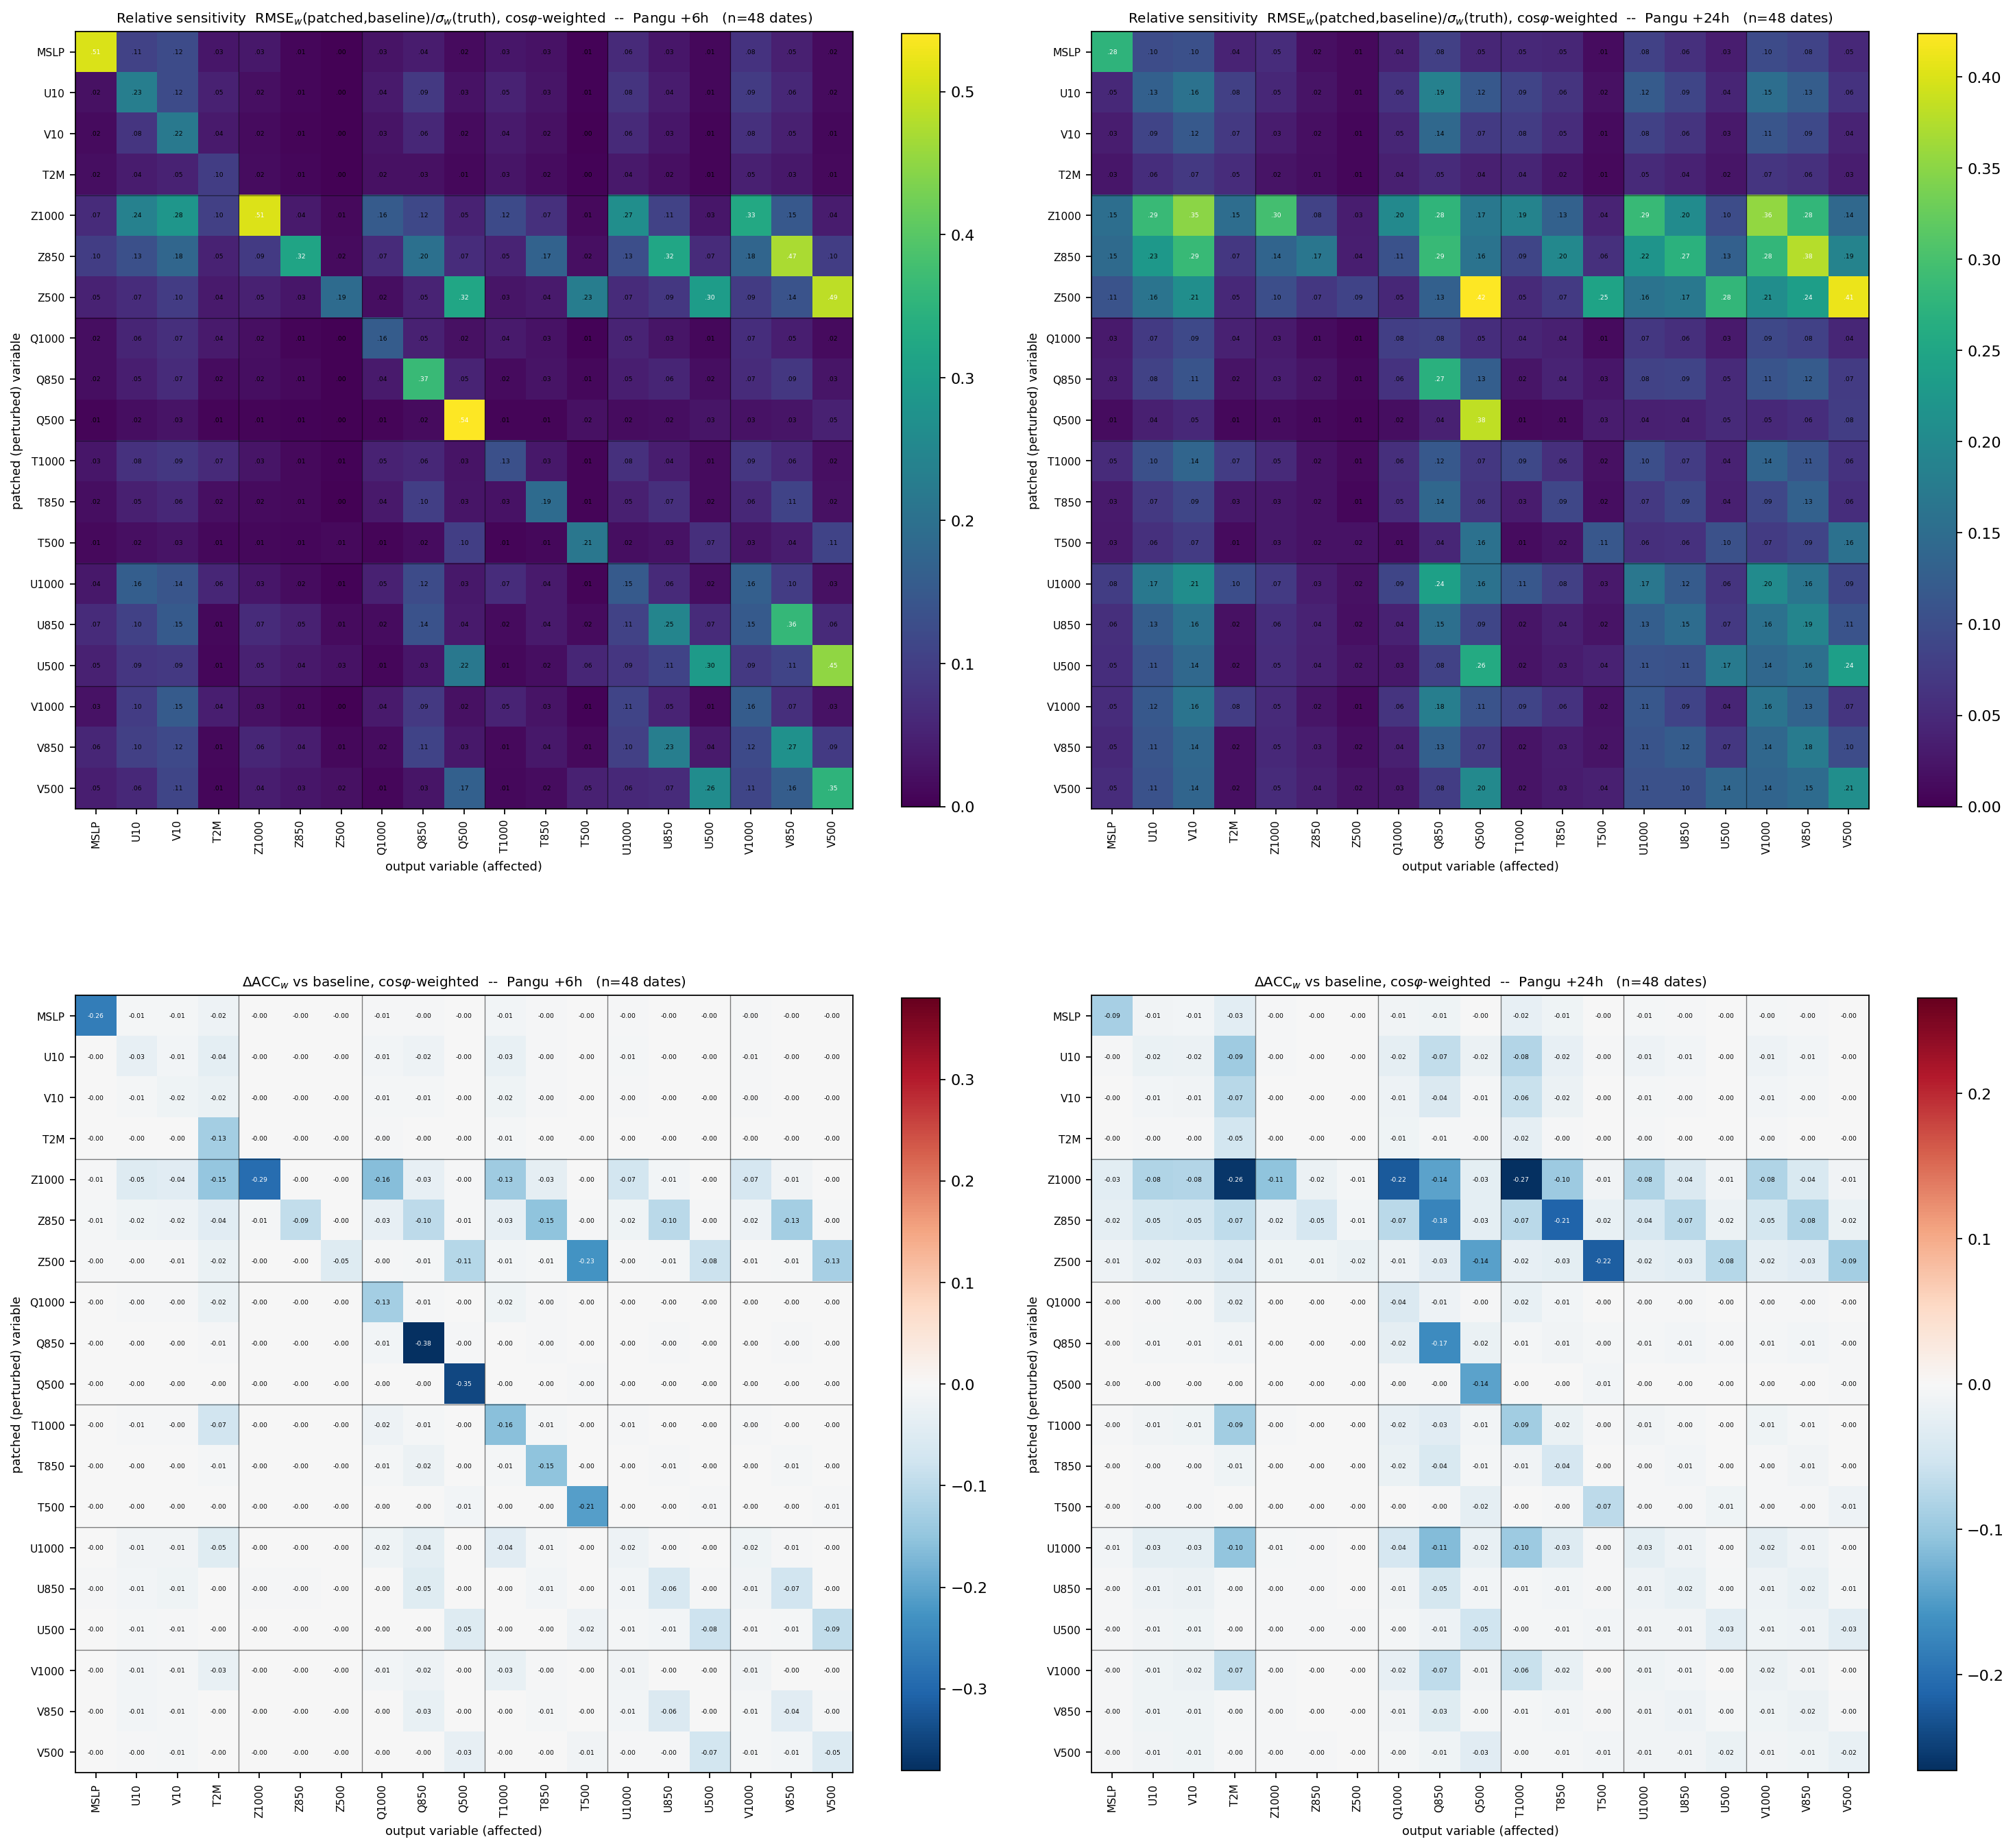
\includegraphics[width=\linewidth]{../../figures/patching_matrices/matrix_19var_pangu_n48_weighted.png}
\caption{Pangu-Weather: полные взвешенные по площади матрицы относительной чувствительности и $\Delta$ACC на +6 и +24 ч ($n=48$).}
\end{figure}

\begin{figure}[p]
\centering
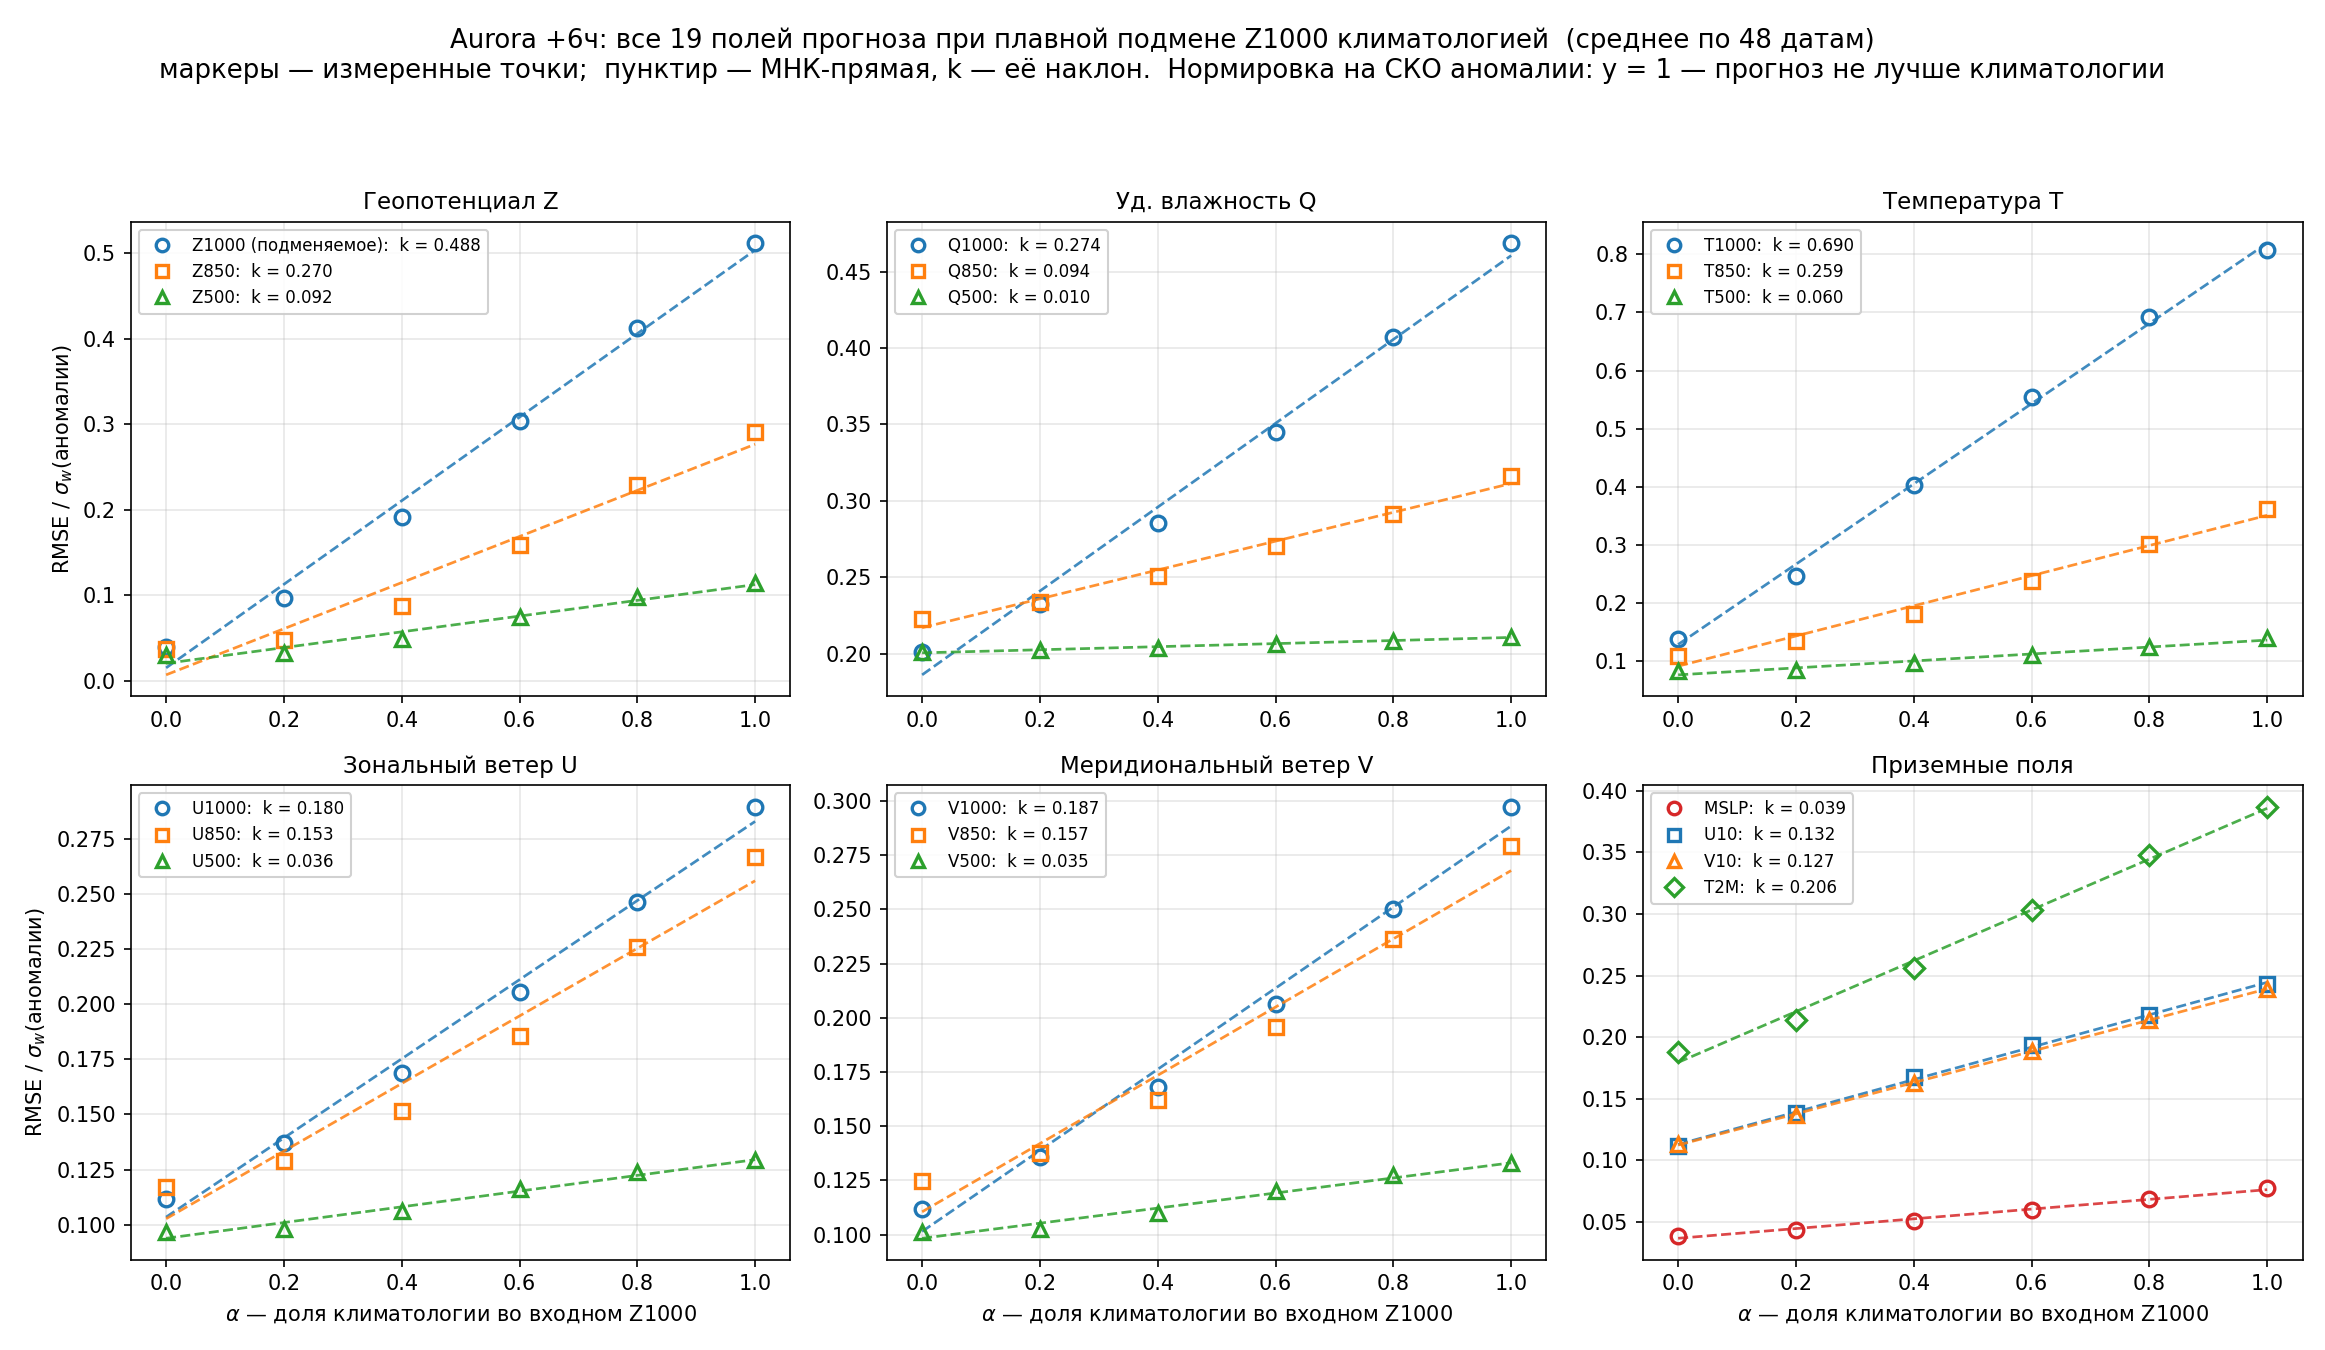
\includegraphics[width=\linewidth]{../../figures/dose_response/dose_panels_anom_Z1000_lead6_aurora_n48.png}
\caption{Aurora +6 ч: dose-response всех 19 выходов при смешивании $Z1000$ с климатологией.}
\end{figure}

\begin{figure}[p]
\centering
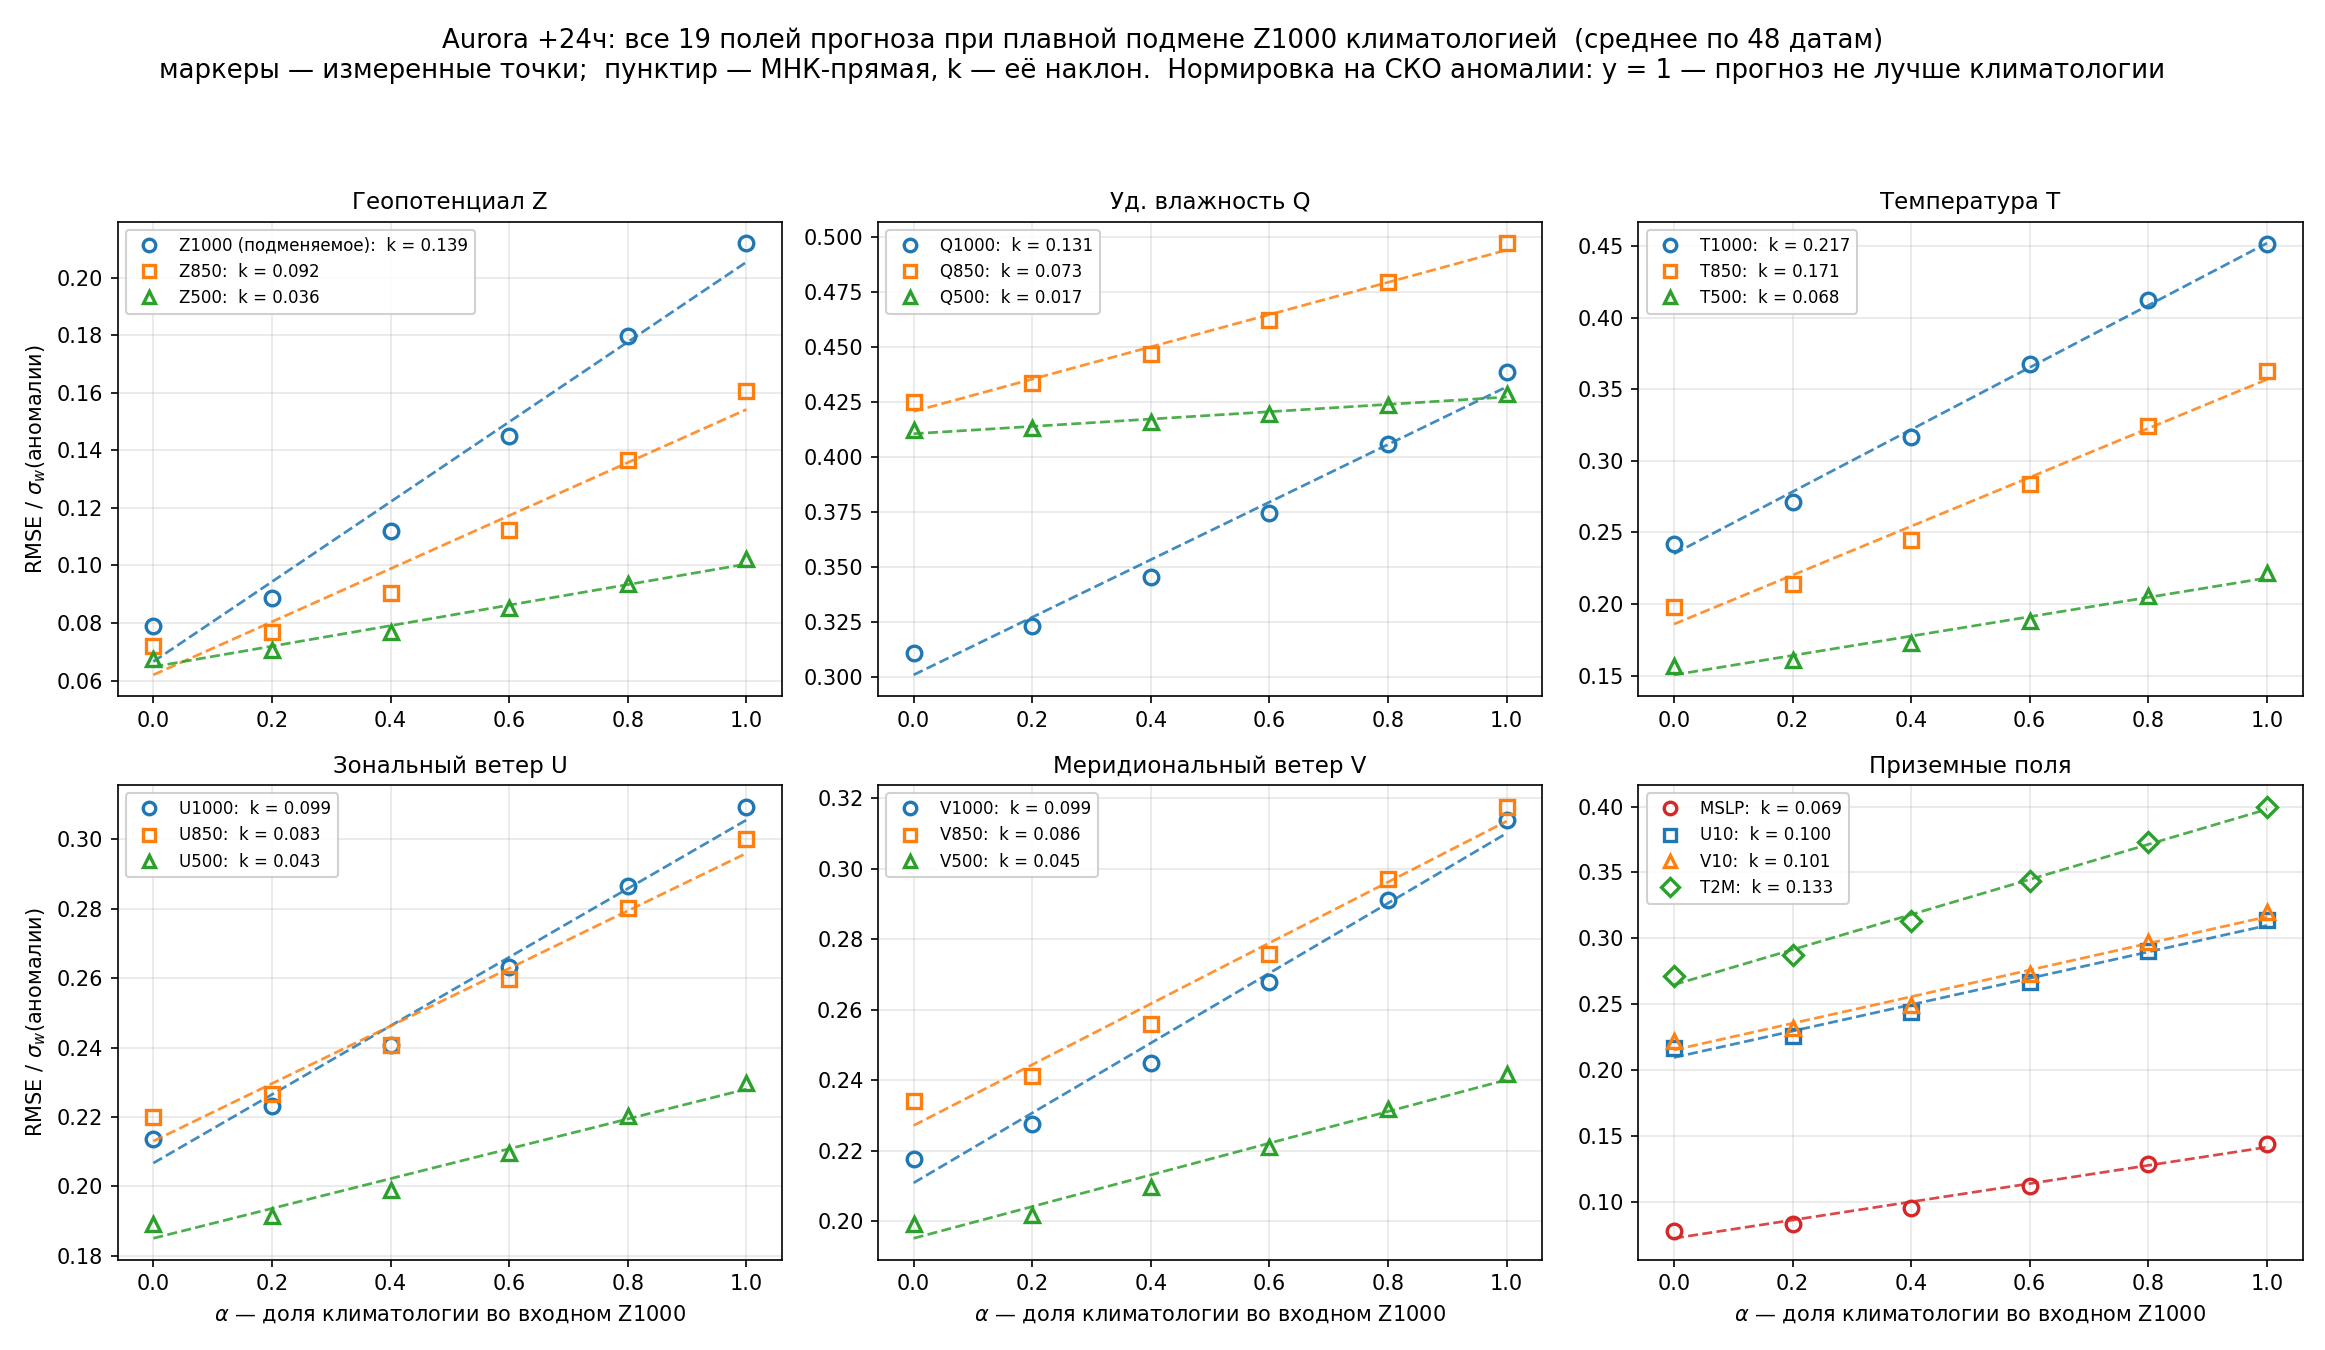
\includegraphics[width=\linewidth]{../../figures/dose_response/dose_panels_anom_Z1000_lead24_aurora_n48.png}
\caption{Aurora +24 ч: dose-response всех 19 выходов при смешивании $Z1000$ с климатологией.}
\end{figure}

\begin{figure}[p]
\centering
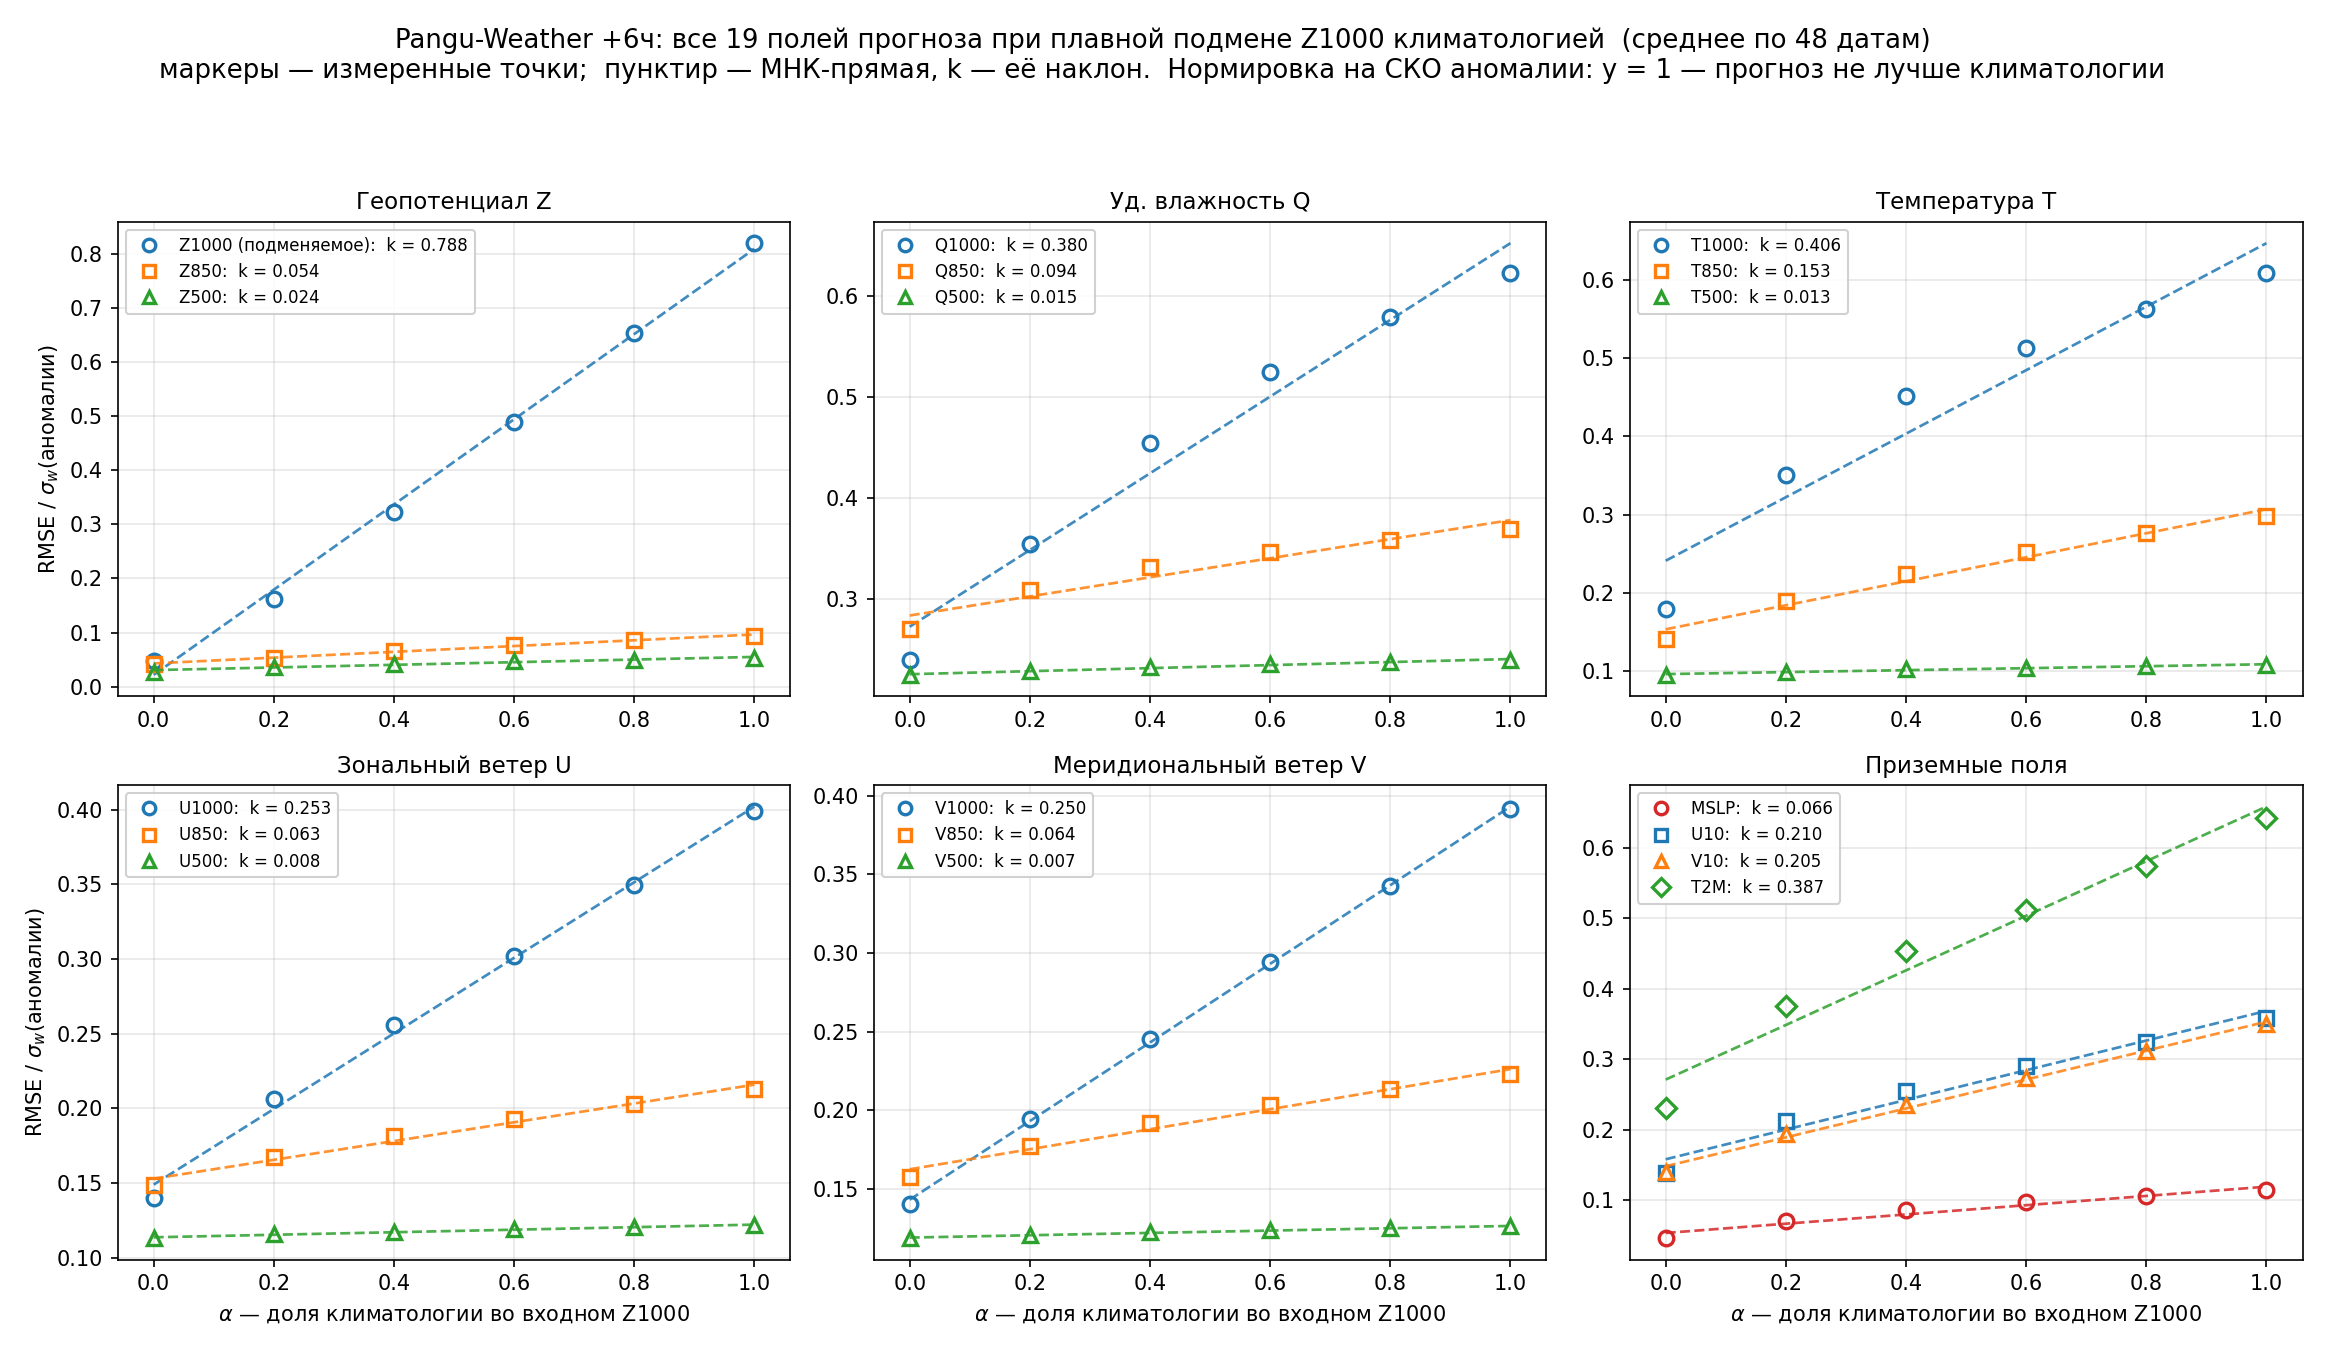
\includegraphics[width=\linewidth]{../../figures/dose_response/dose_panels_anom_Z1000_lead6_pangu_n48.png}
\caption{Pangu-Weather +6 ч: dose-response всех 19 выходов. На этом сроке наклон $T1000$ меньше, чем у Aurora, а наклоны ветра нижнего уровня и $T2M$ больше.}
\end{figure}

\begin{figure}[p]
\centering
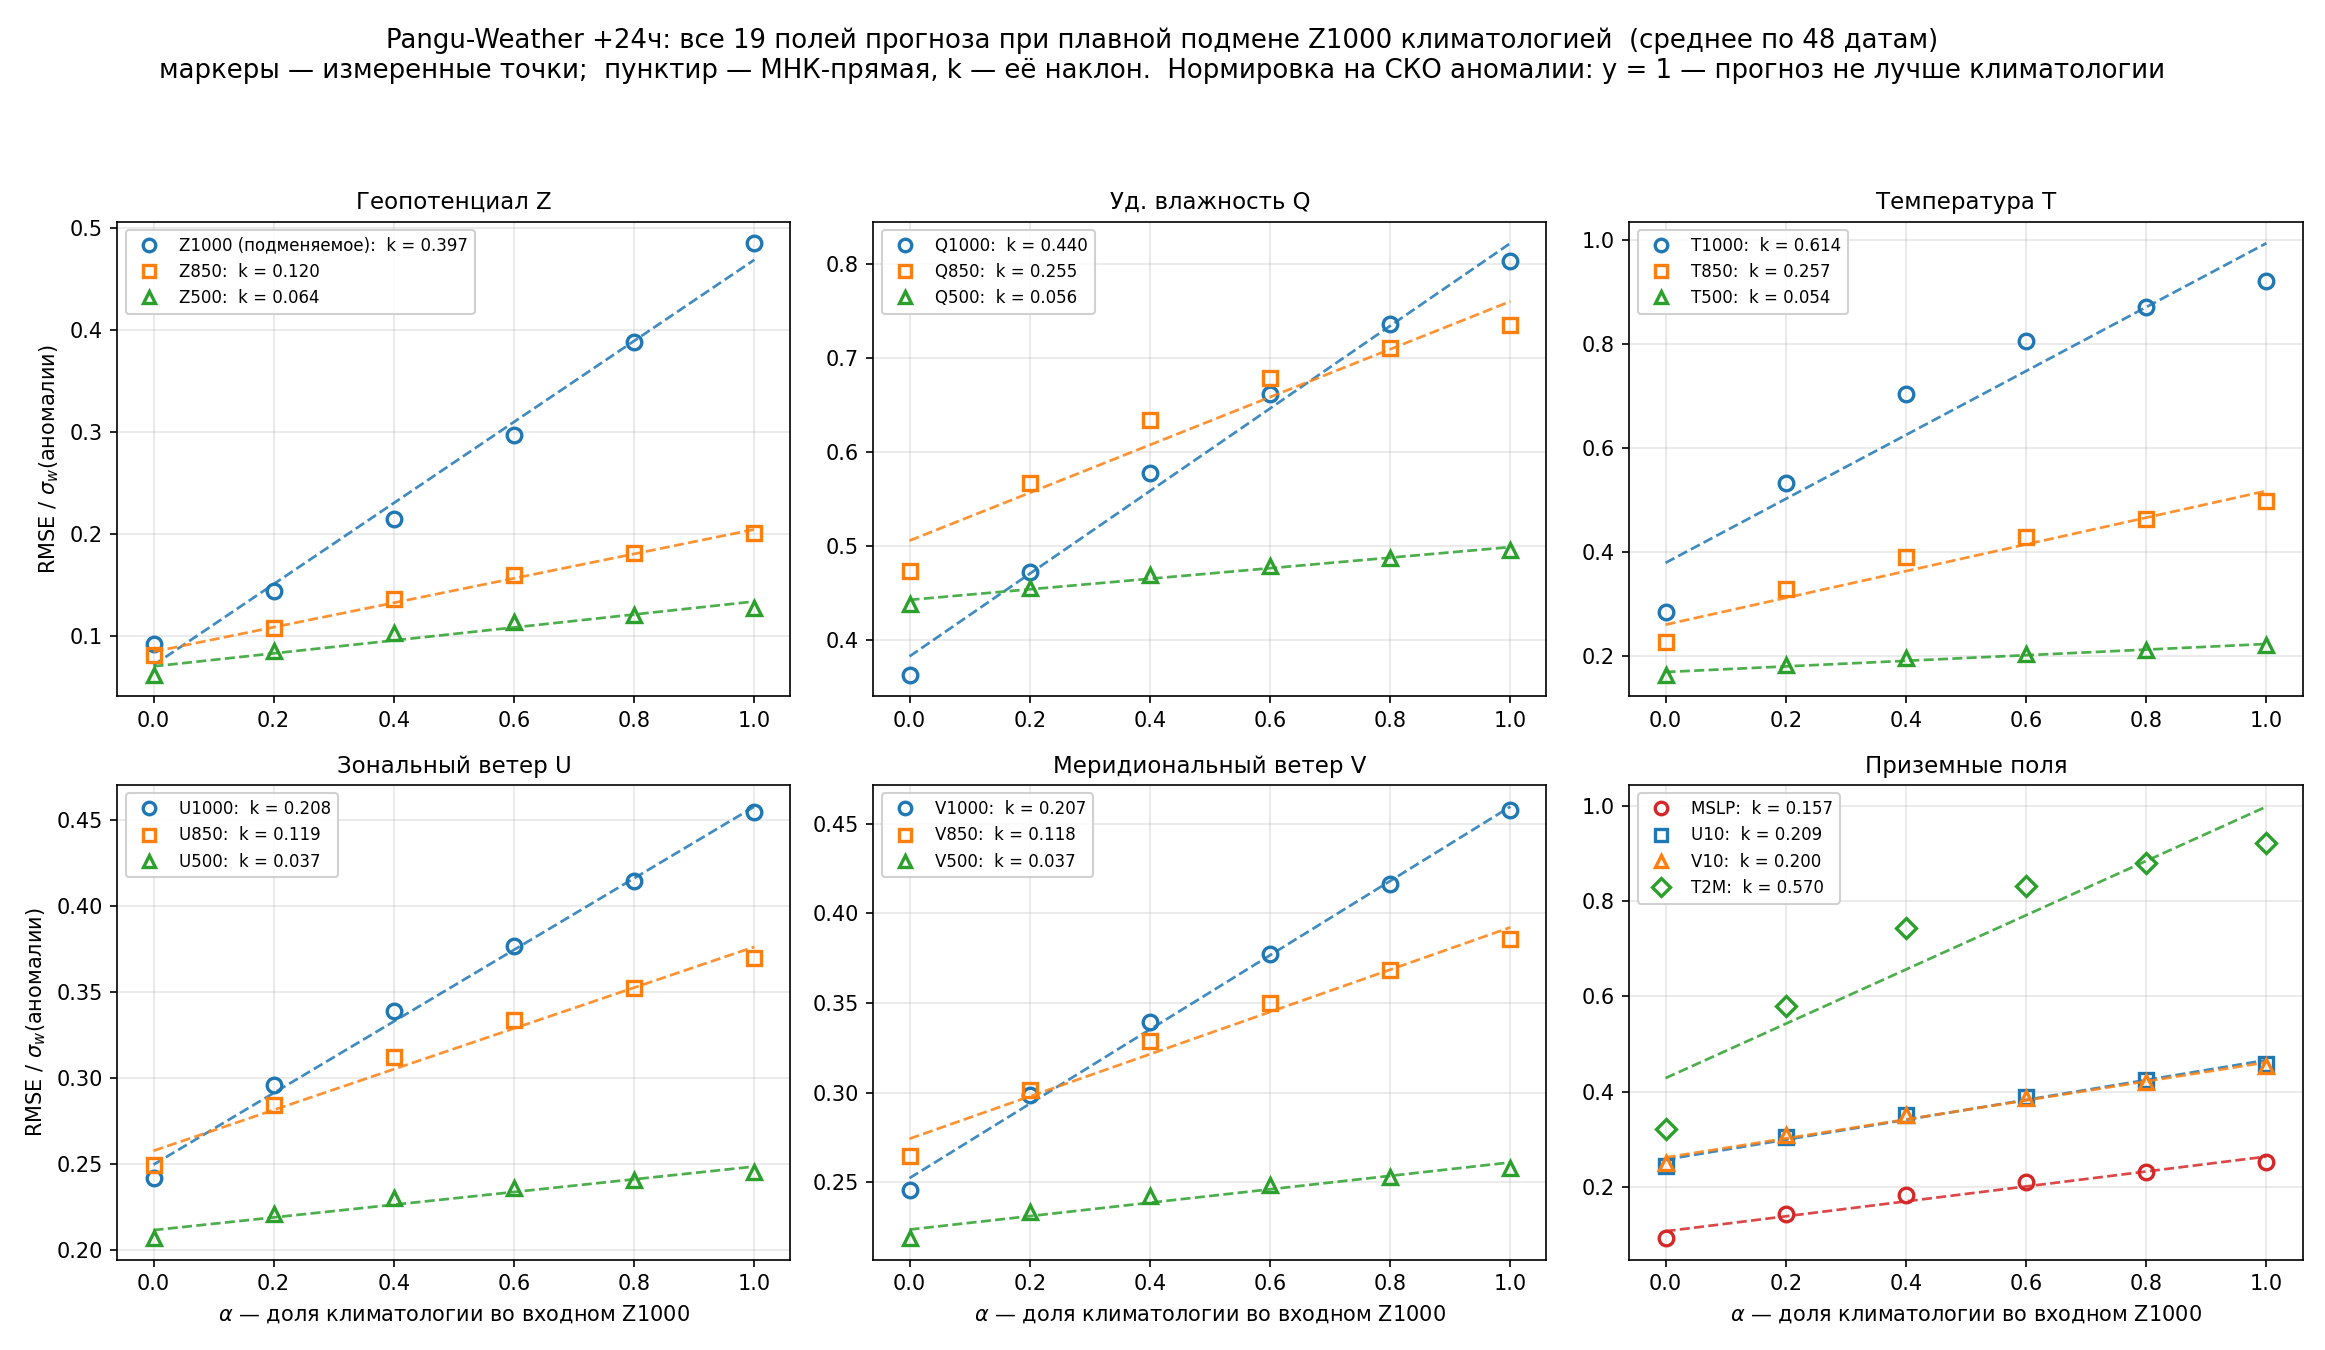
\includegraphics[width=\linewidth]{../../figures/dose_response/dose_panels_anom_Z1000_lead24_pangu_n48.png}
\caption{Pangu-Weather +24 ч: dose-response всех 19 выходов. Наклоны $T1000$ и $T2M$ растут с заблаговременностью, в отличие от Aurora.}
\end{figure}

\begin{figure}[p]
\centering
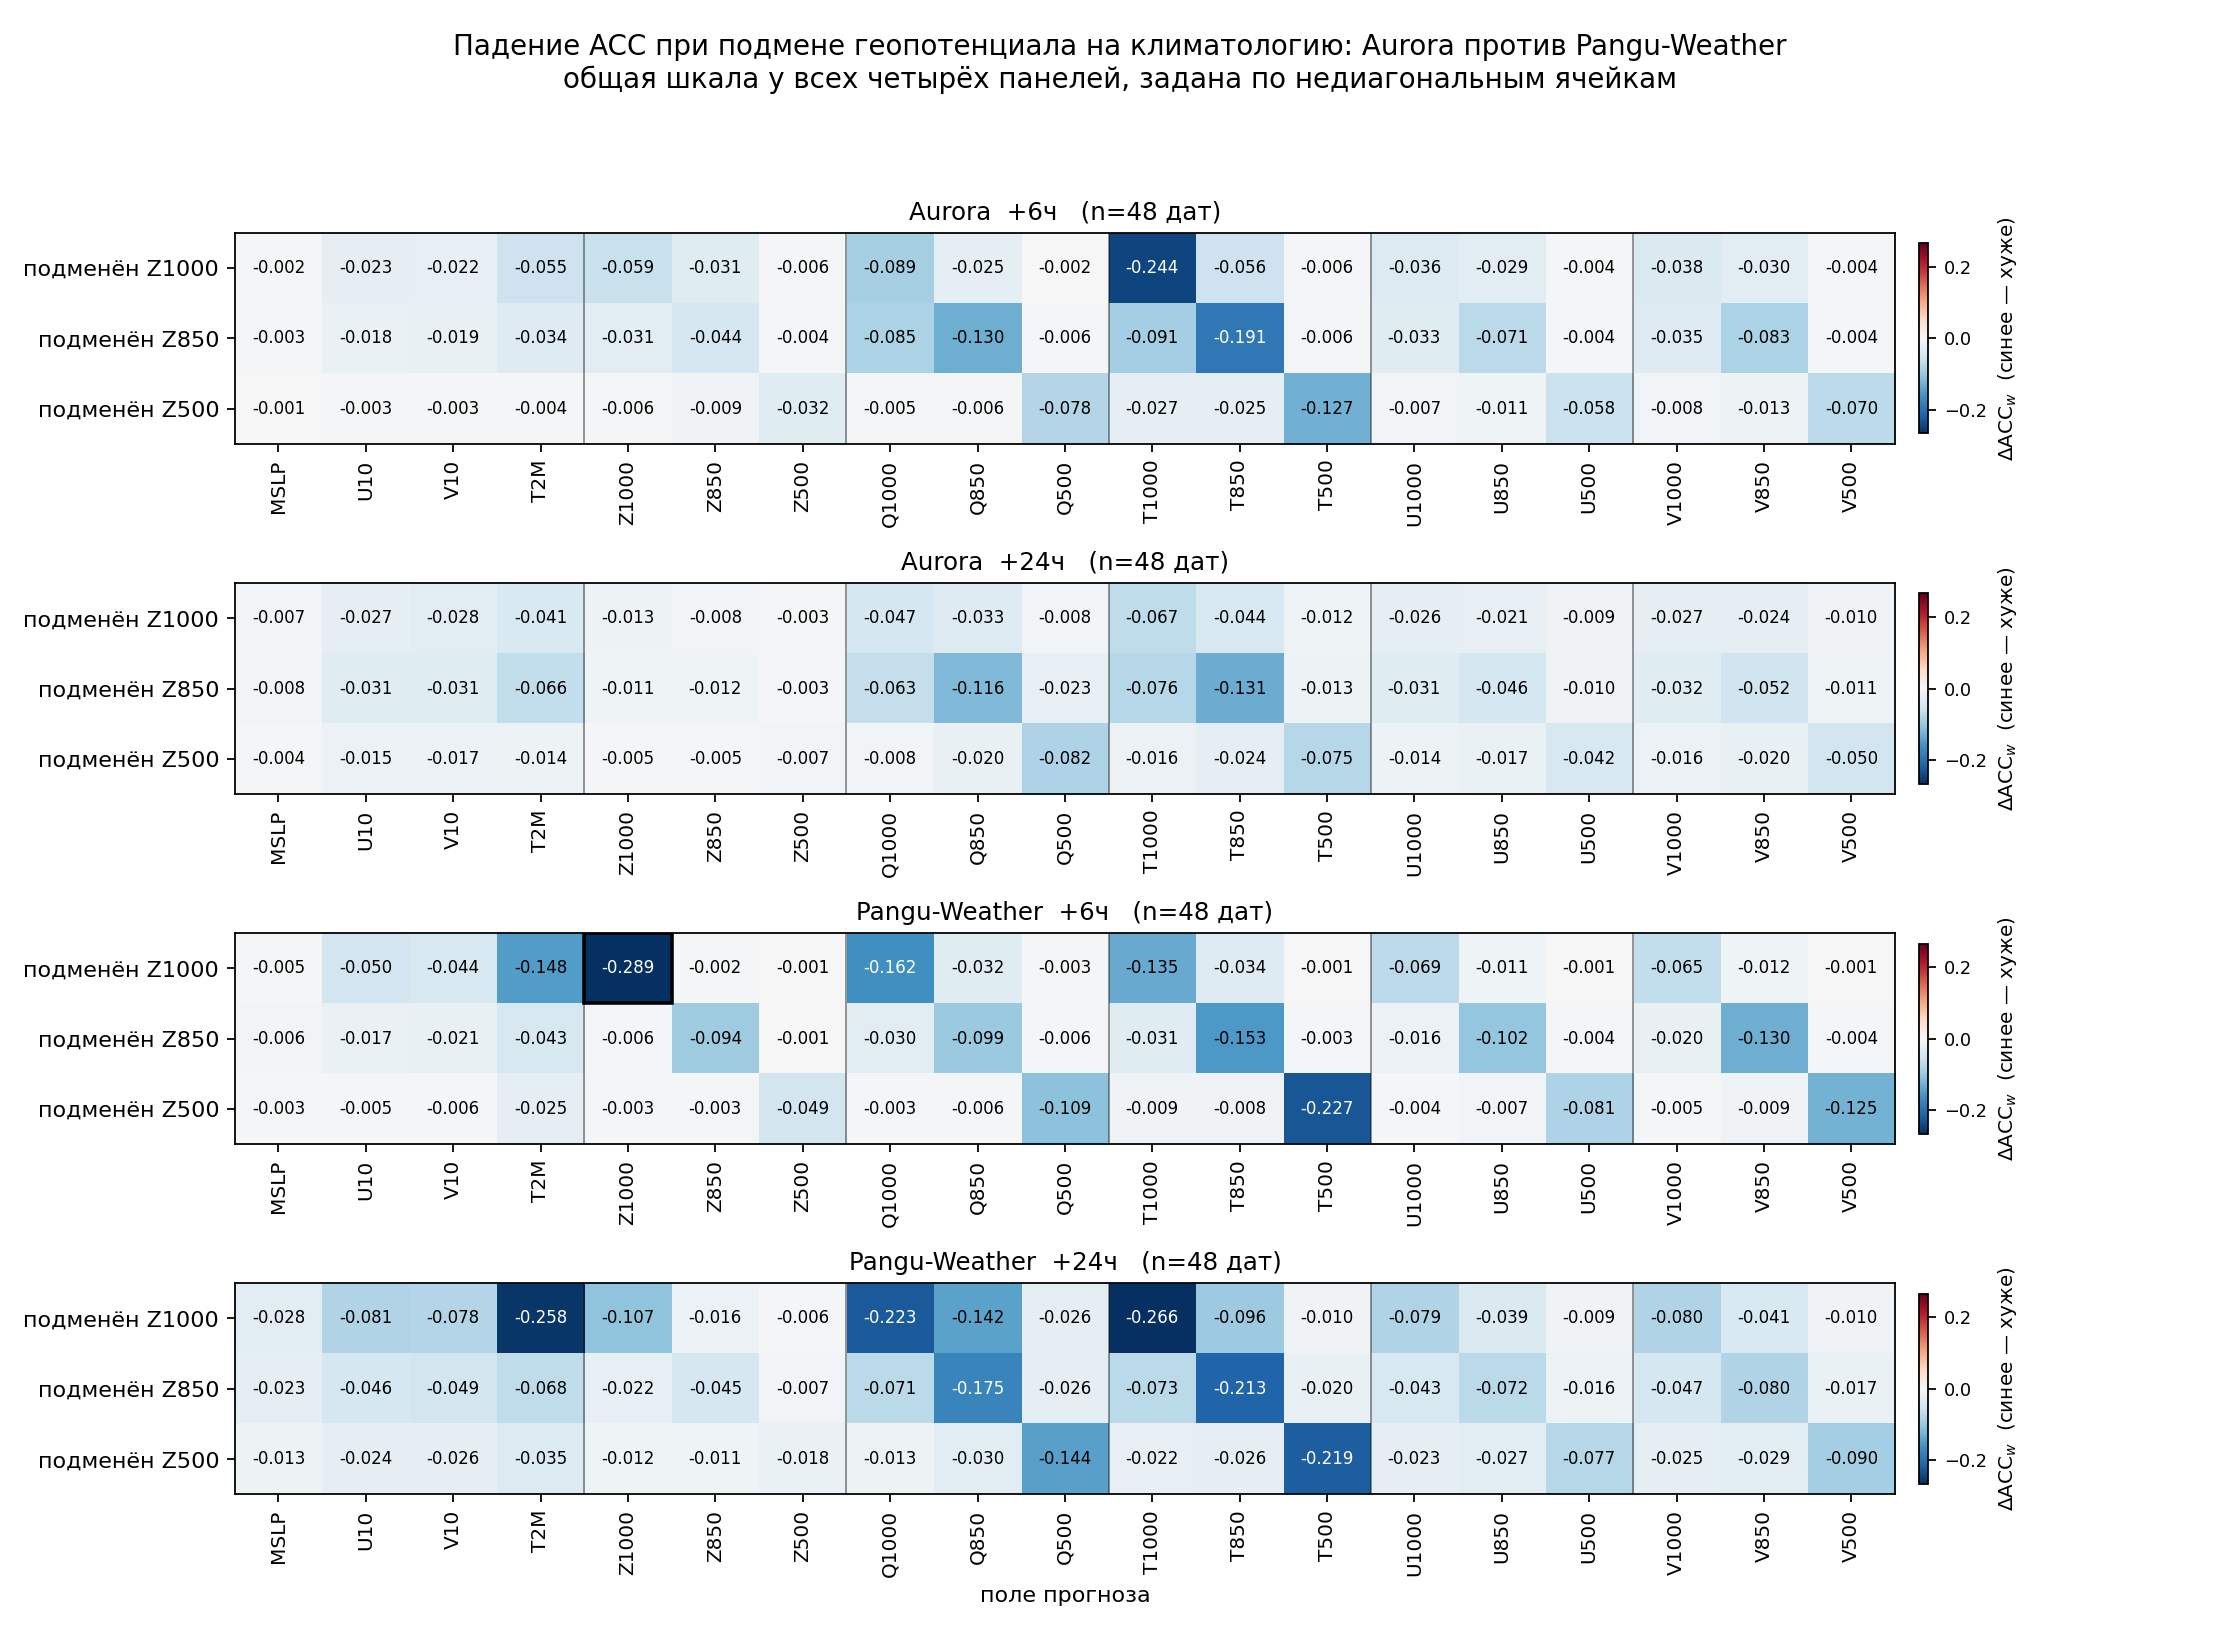
\includegraphics[width=\linewidth]{../../figures/patching_matrices/acc_strip_Z_both_n48.png}
\caption{Строки $\Delta\acc$ для замены $Z1000$, $Z850$ и $Z500$ в обеих моделях. У каждой панели шкала полной исходной матрицы; сравнивать следует числа, а не насыщенность цвета.}
\end{figure}

\begin{figure}[p]
\centering
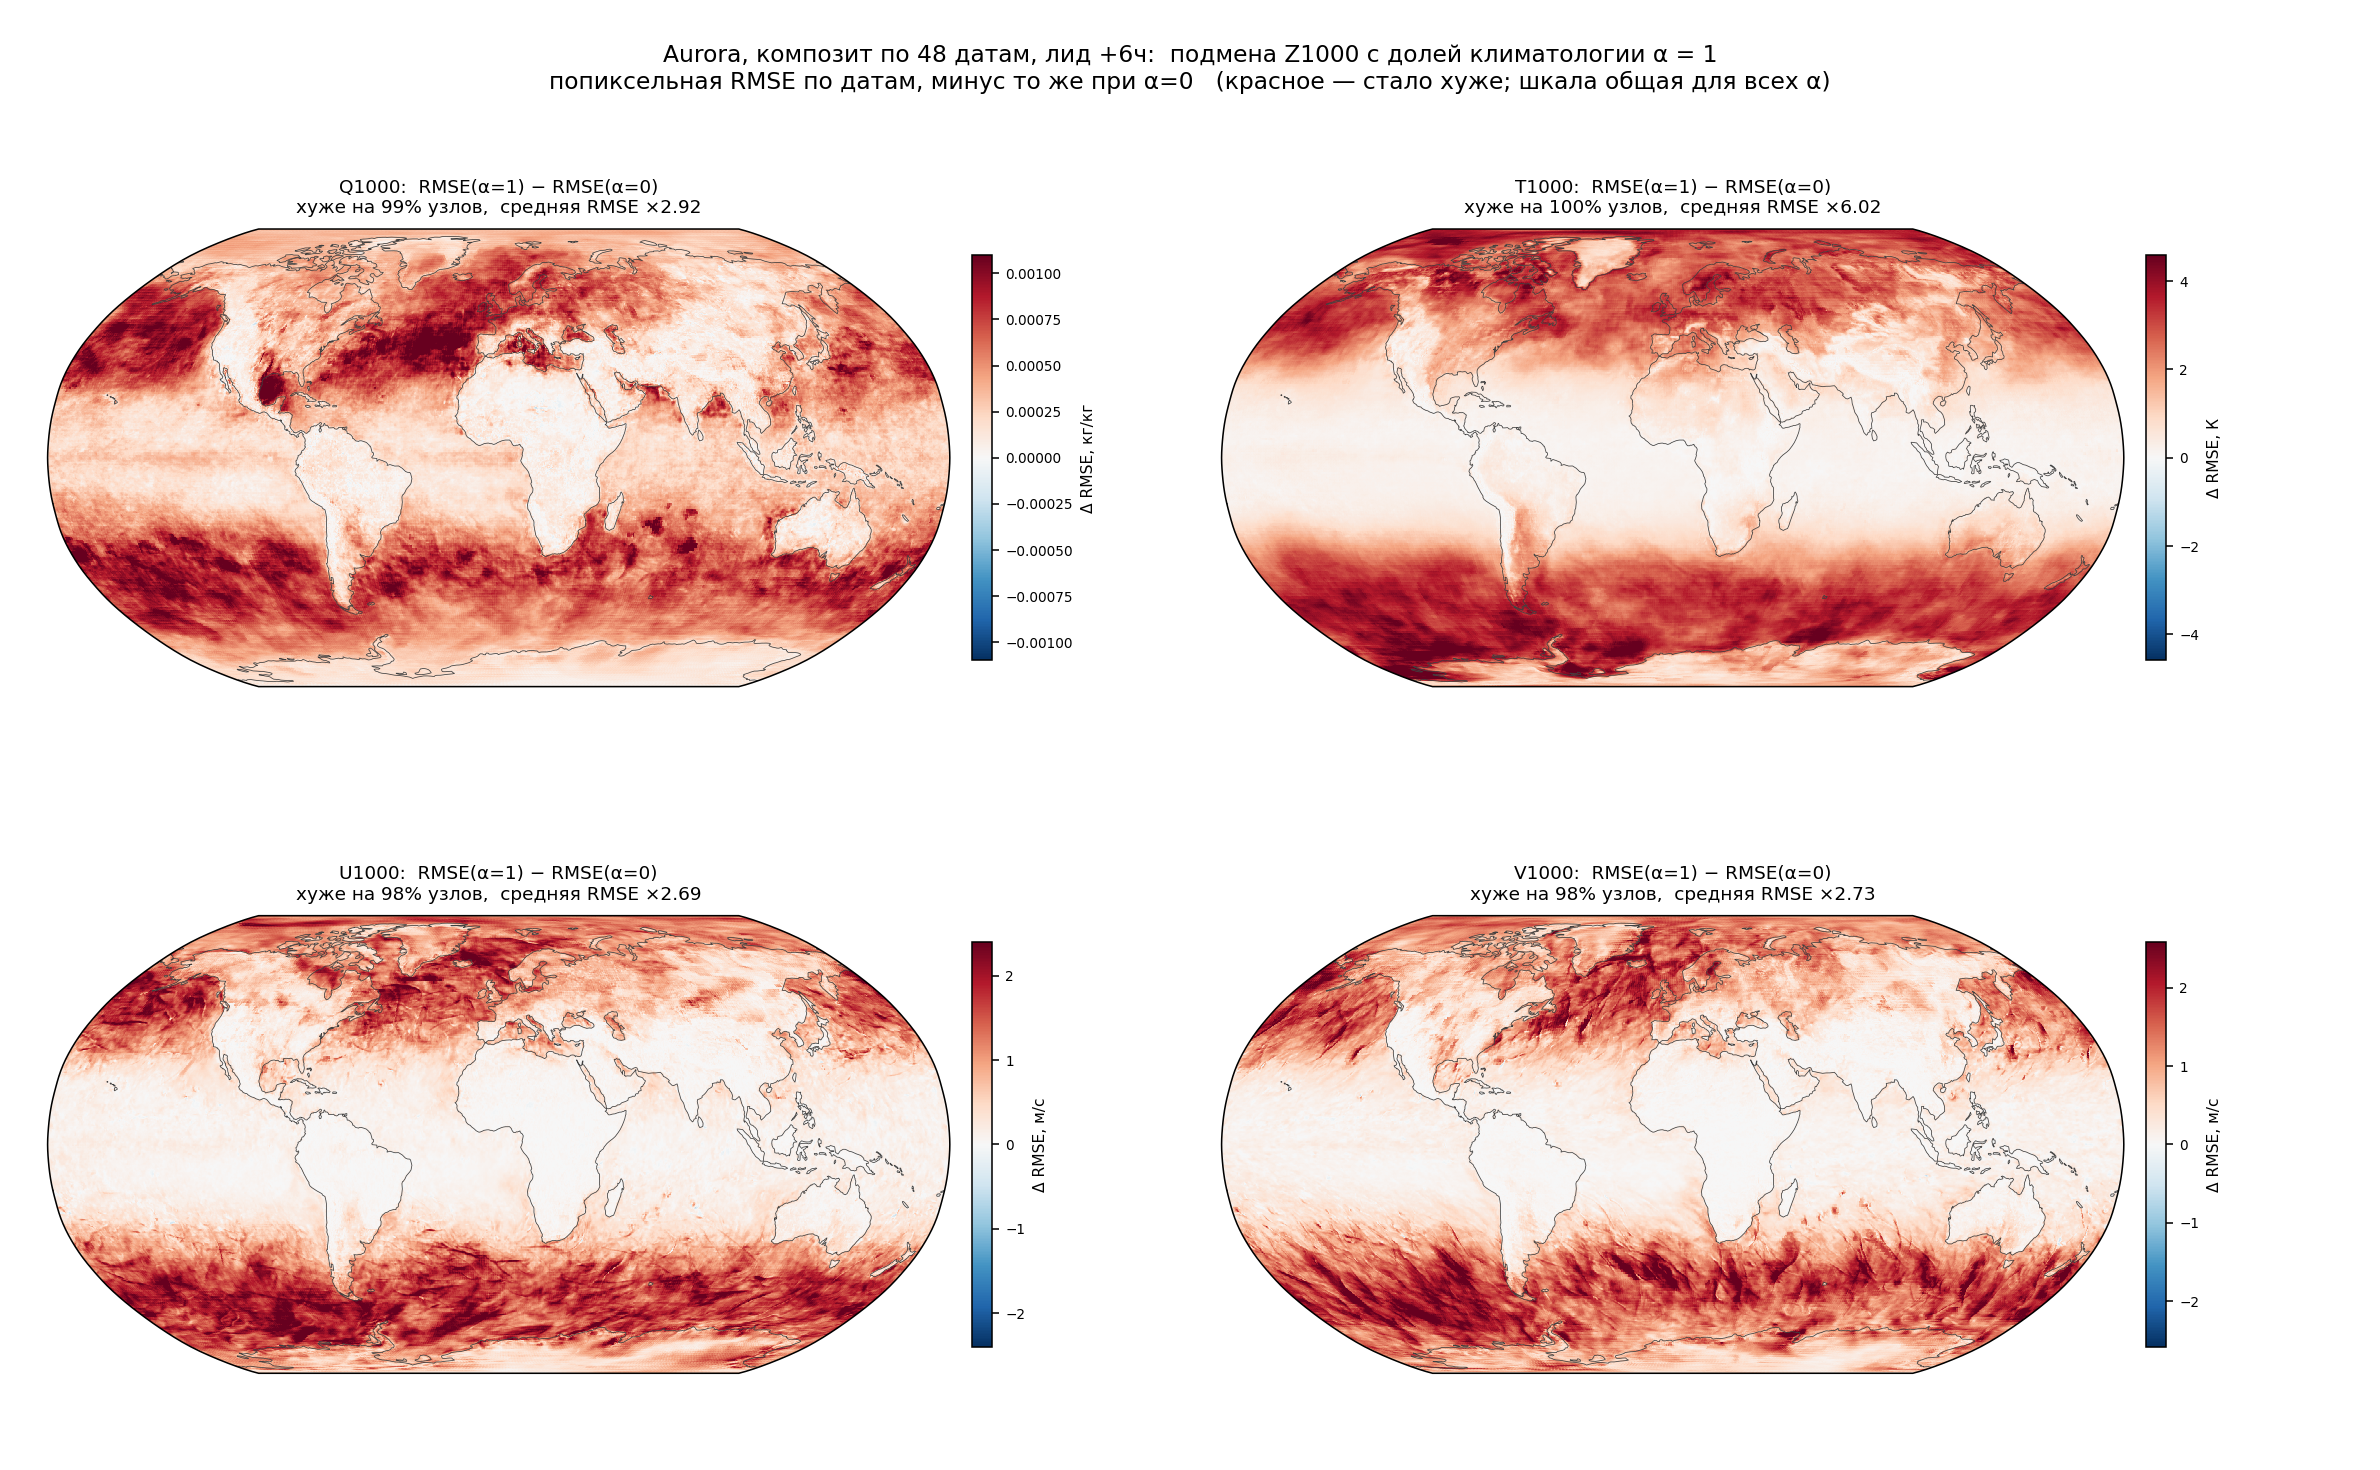
\includegraphics[width=\linewidth]{../../figures/bias_maps/composite_bias_Z1000_lead6_alpha1_n48.png}
\caption{Aurora: пространственный композит при полной замене $Z1000$ ($\alpha=1$, +6 ч). Красный цвет означает рост временной RMSE относительно базового прогноза.}
\end{figure}

\begin{figure}[p]
\centering
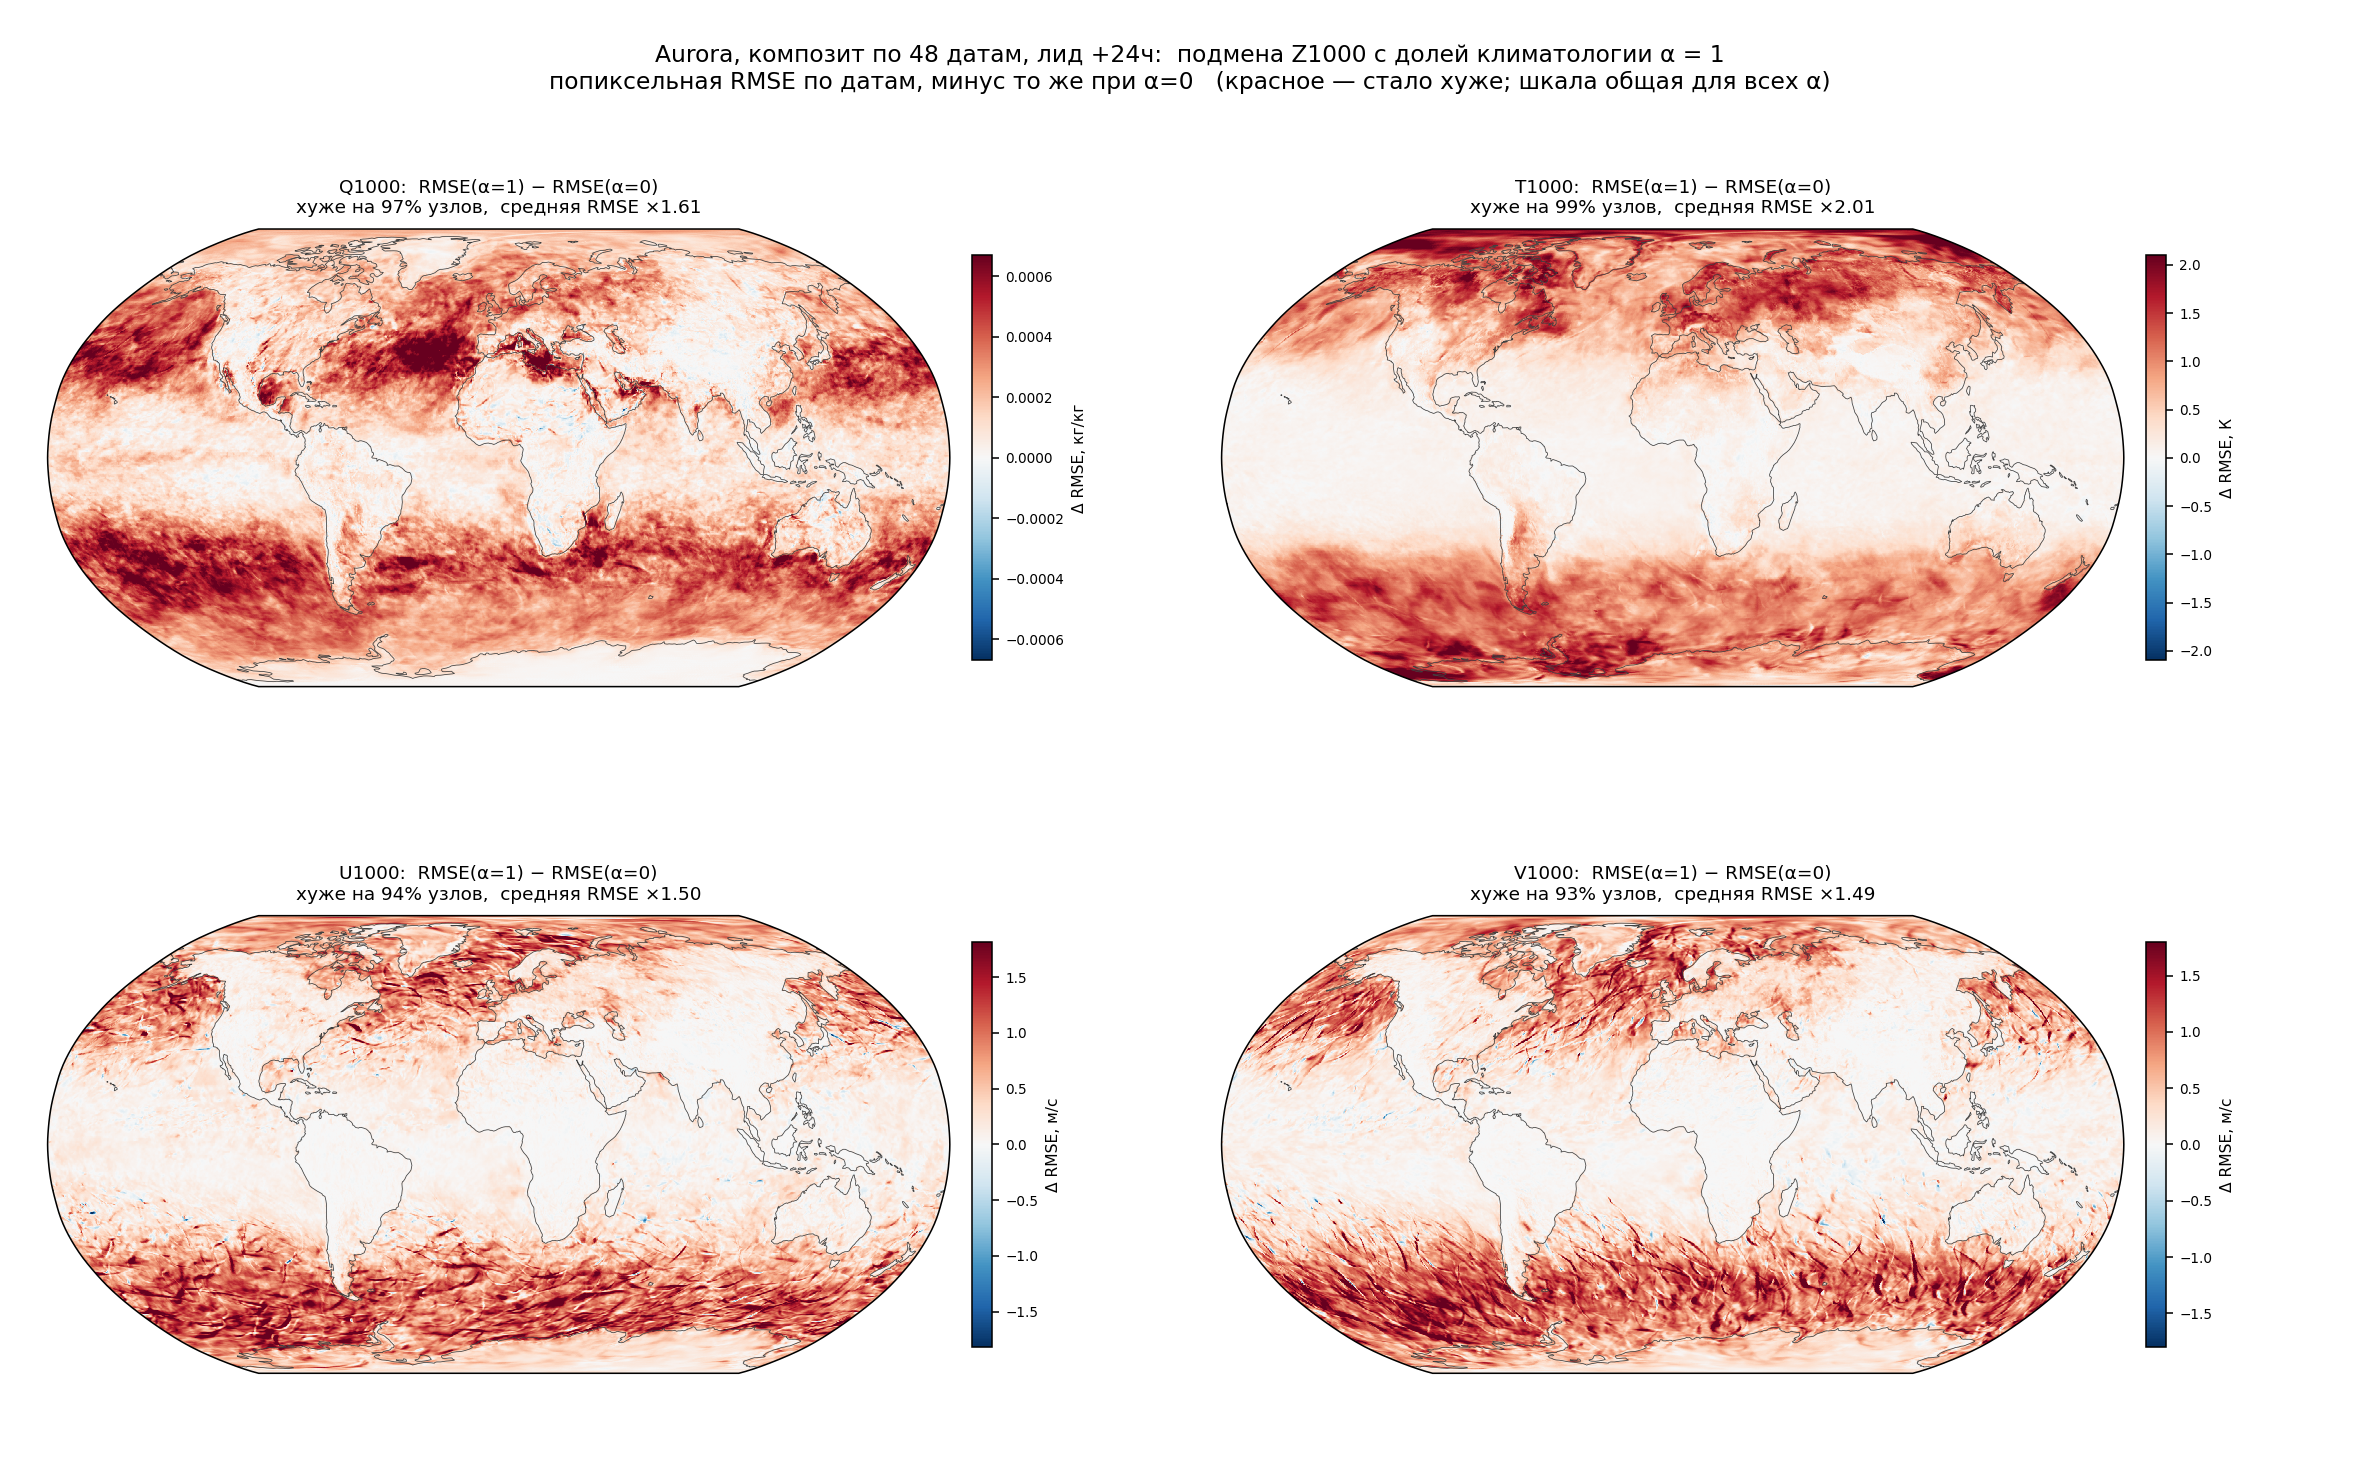
\includegraphics[width=\linewidth]{../../figures/bias_maps/composite_bias_Z1000_lead24_alpha1_n48.png}
\caption{Aurora, +24 ч. Отклик слабее, чем на +6 ч, но остается положительным в 93--99\% узлов для четырех показанных полей.}
\end{figure}

\begin{figure}[p]
\centering
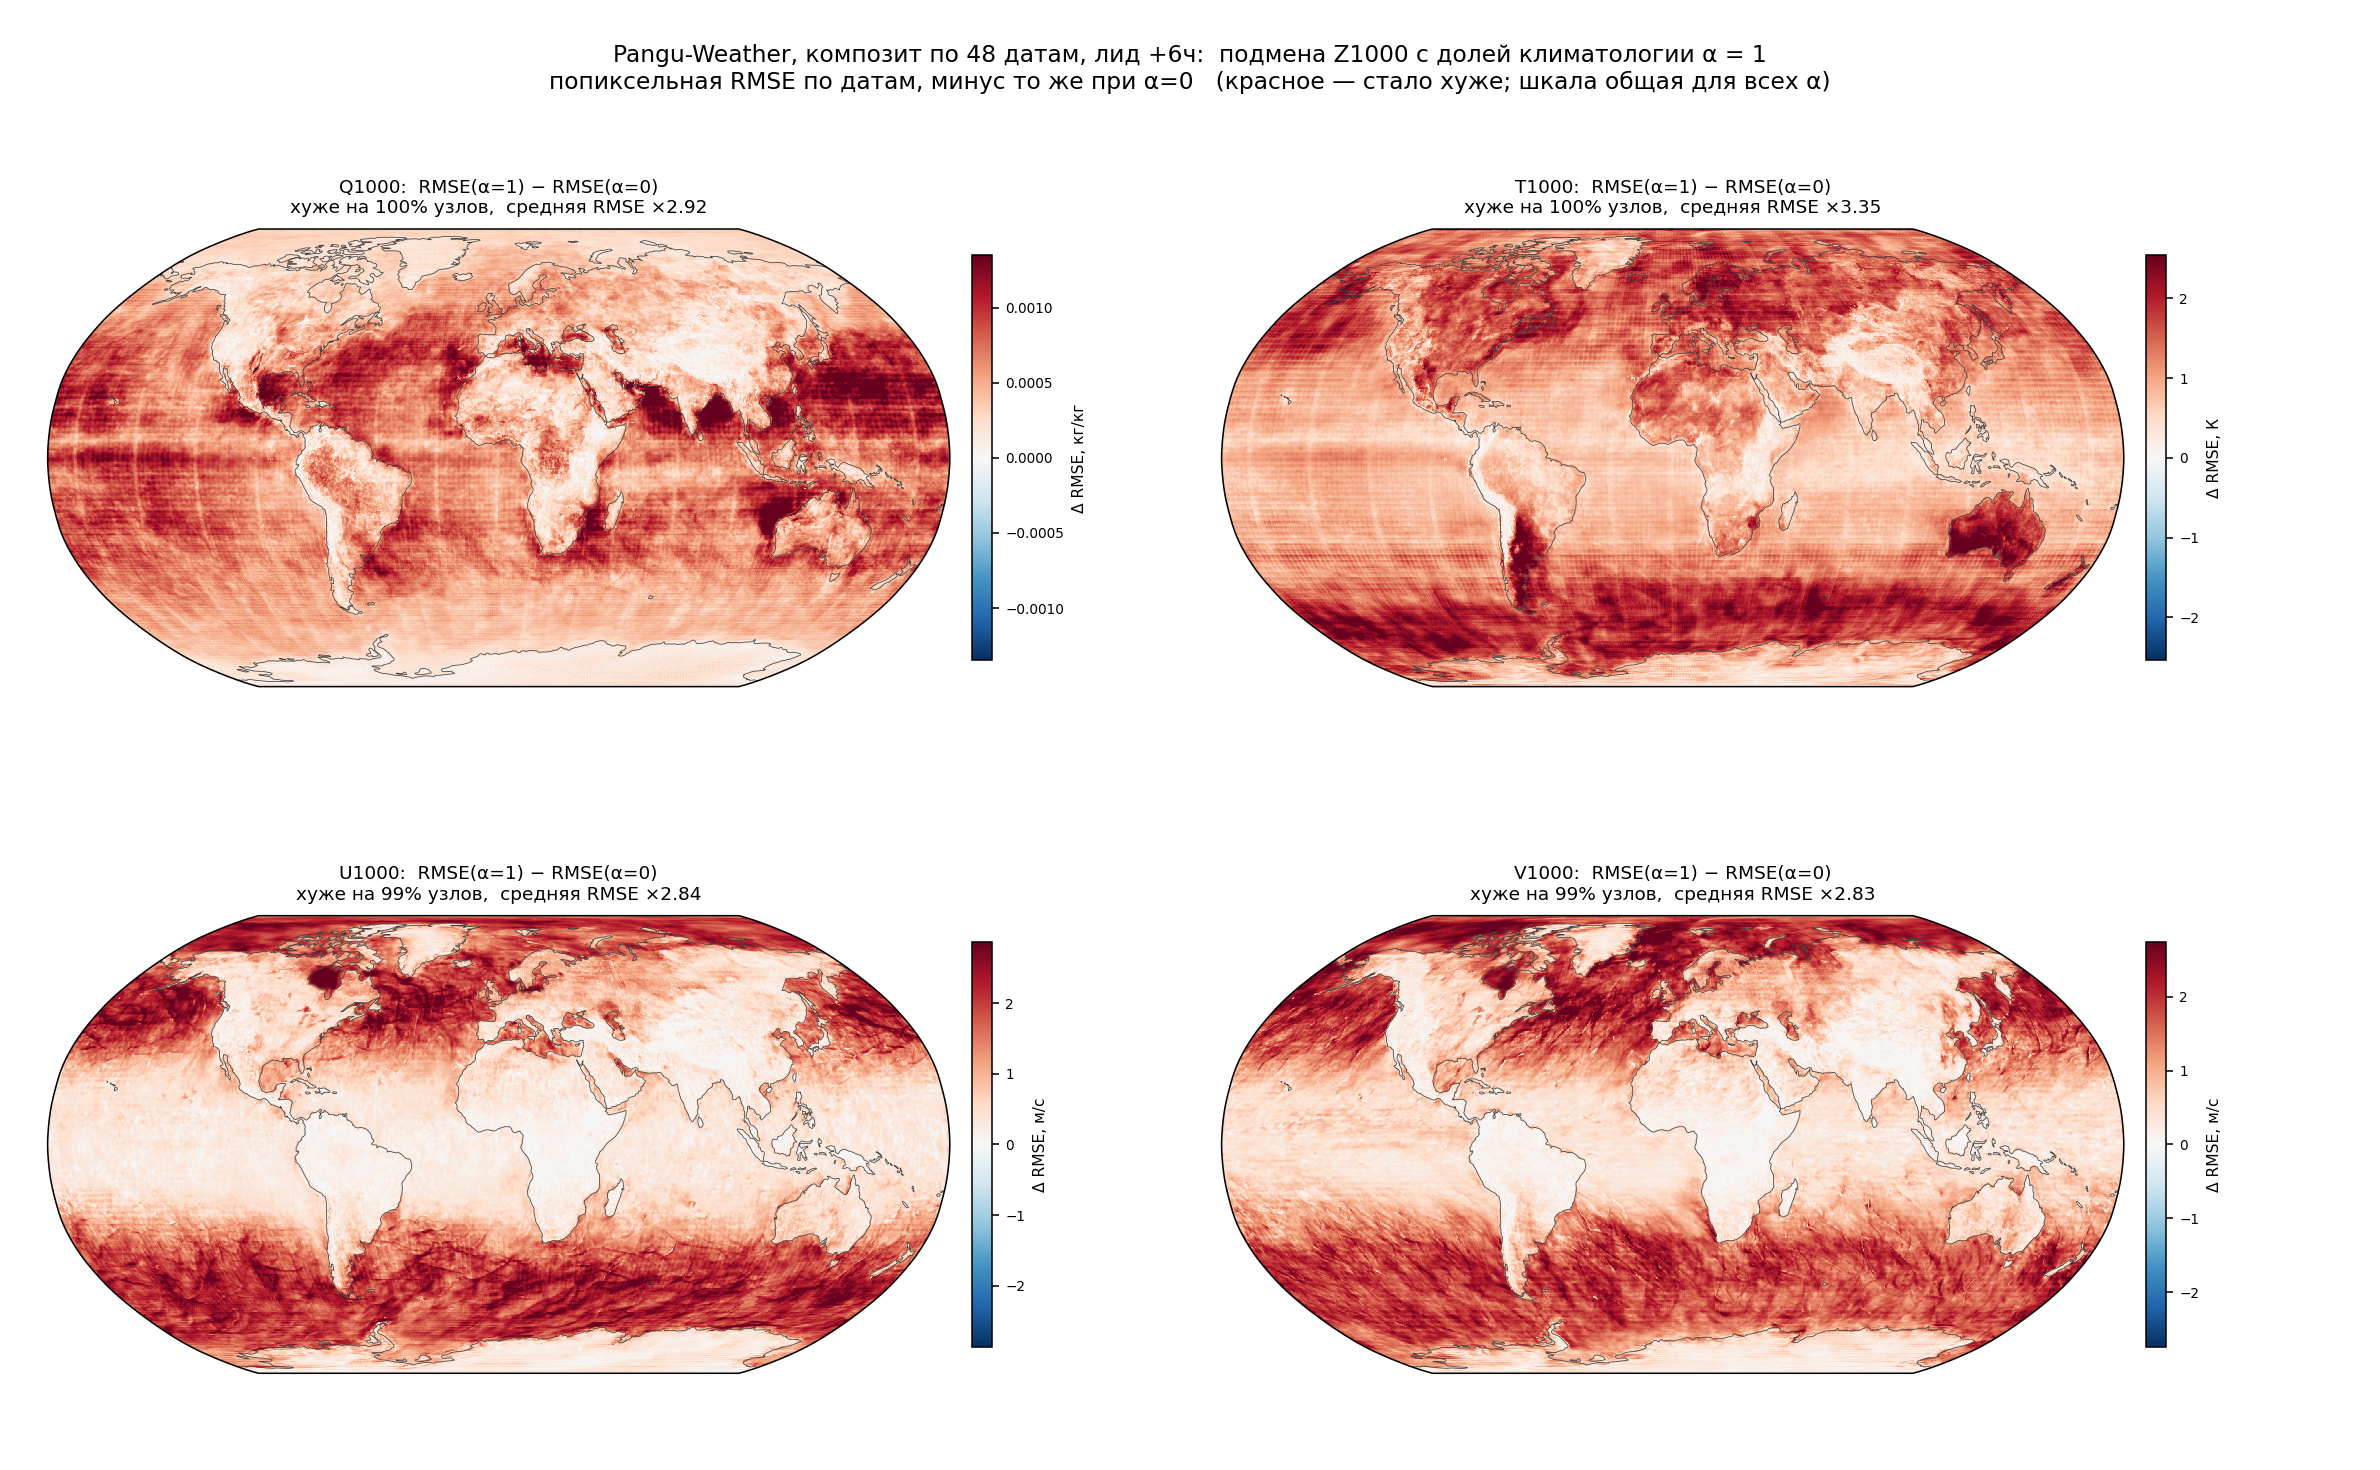
\includegraphics[width=\linewidth]{../../figures/bias_maps/composite_bias_pangu_Z1000_lead6_alpha1_n48.png}
\caption{Pangu-Weather, +6 ч. Ошибка всех четырех показанных полей возрастает в 99--100\% узлов.}
\end{figure}

\begin{figure}[p]
\centering
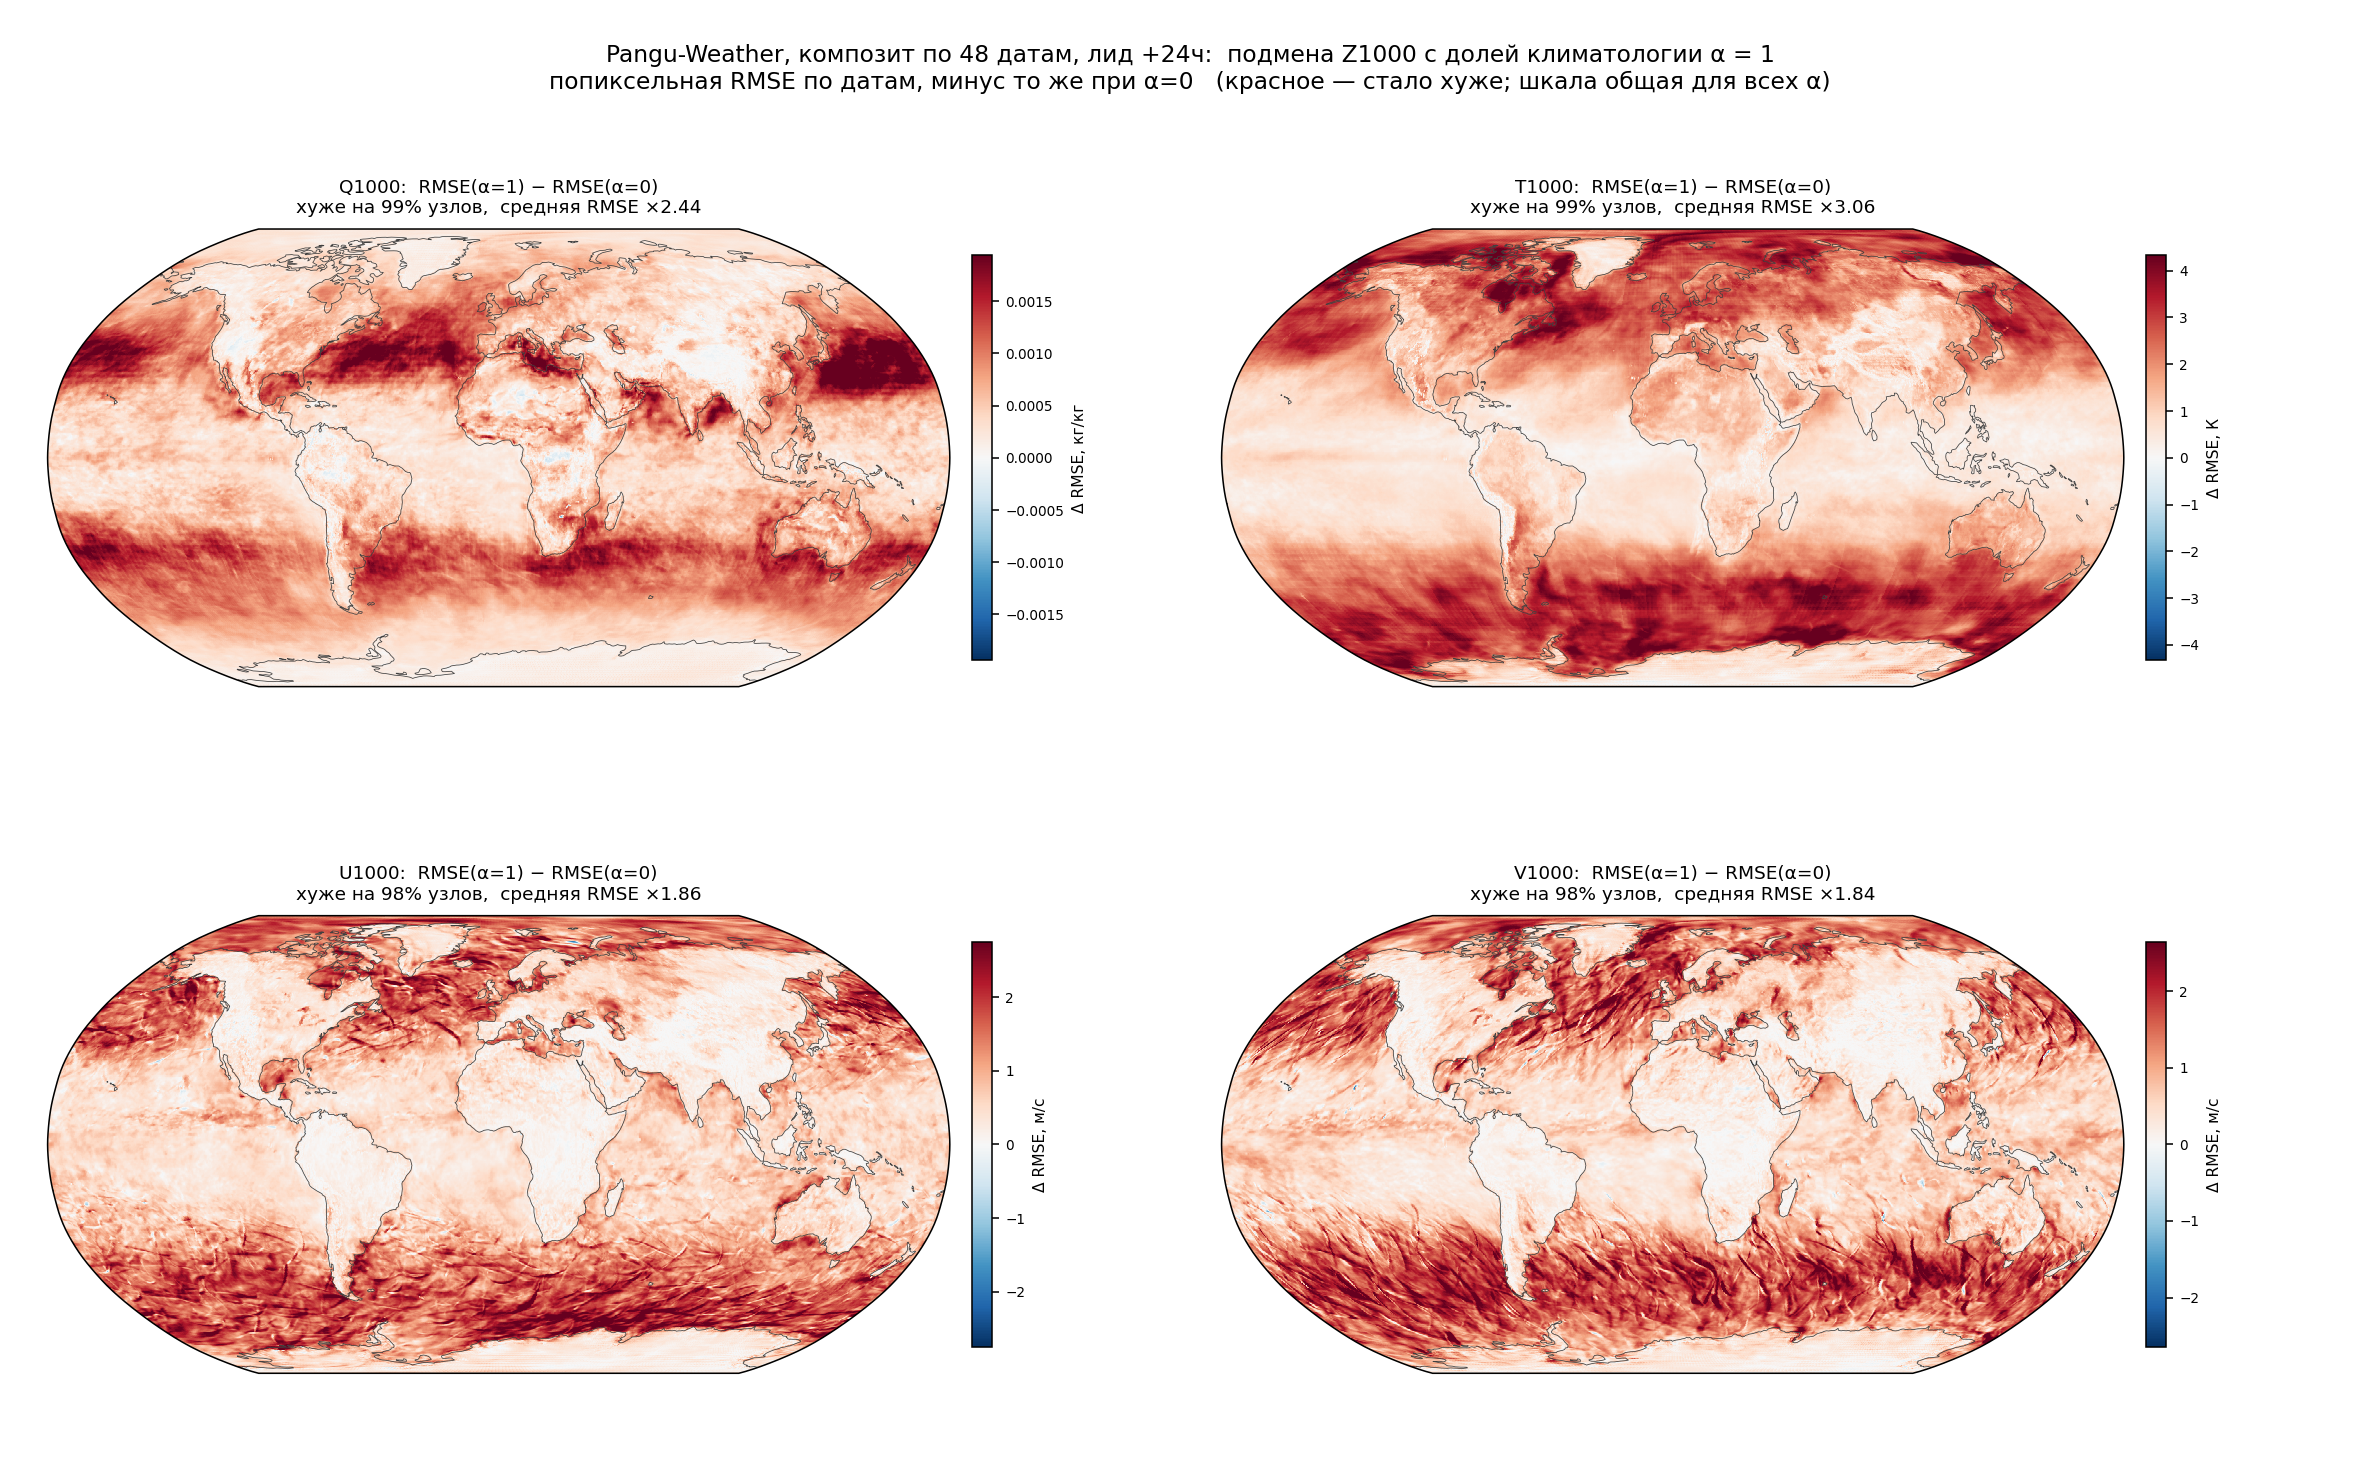
\includegraphics[width=\linewidth]{../../figures/bias_maps/composite_bias_pangu_Z1000_lead24_alpha1_n48.png}
\caption{Pangu-Weather, +24 ч. Отношение средней по узлам RMSE $T1000$ равно $3.06\times$ против $2.01\times$ у Aurora.}
\end{figure}

\end{document}
